\documentclass[11pt, a4paper, twoside]{report}
%\usepackage[a4paper, portrait, margin=1in]{geometry}

\usepackage{import}

\usepackage[utf8]{inputenc}
\usepackage{amsmath}
\usepackage{amssymb}
\usepackage{amsthm}
\usepackage{multicol}
\usepackage{multirow}

\usepackage{fontspec}
\usepackage{unicode-math}

\usepackage[
    style=authoryear-icomp,
    citestyle=authoryear-icomp
]{biblatex}
\addbibresource{thesis.bib}
\addbibresource{Iris-Information-Obfuscation/references.bib}

\DeclareLabeldate[online]{%
  \field{date}
  \field{year}
  \field{eventdate}
  \field{origdate}
  \field{urldate}
}

\usepackage{hyperref}
\usepackage{cleveref}
\usepackage{csquotes}
\usepackage{caption}
\usepackage{subcaption}
\usepackage[toc, acronym]{glossaries}
\usepackage{nomencl}

\usepackage{todonotes}

\usepackage{quotchap}
\usepackage{tikz}
\usepackage{pgfplots}
\usepackage{wrapfig}
\pgfplotsset{compat=1.16}
\usetikzlibrary{shapes.geometric, arrows}

\usepackage{booktabs}
\usepackage{fancyhdr}
\pagestyle{fancy}
\fancyhead[LE]{}
\fancyhead[RO]{}

\newtheorem{definition}{Definition}[section]
\newtheorem{theorem}{Theorem}[section]

\newcommand{\norm}[1]{\left\lVert#1\right\rVert}

\tikzstyle{rect} = [rectangle,text centered, minimum width=1cm, minimum height=0.7cm, draw=black, fill=gray!30]

\tikzstyle{circ} = [circle, text centered, draw=black, fill=gray!30]

\tikzstyle{empty} = [text centered, draw=black]

\tikzstyle{arrow} = [thick,->,>=stealth]


\makenoidxglossaries

\newglossaryentry{eye-process}
{
    name={eye information process},
    description={Is any process that uses a human eye as its input and has the aim of extracting some property from its appearance or movements.}
}

%% This code creates the groups
% -----------------------------------------
\usepackage{etoolbox}
\renewcommand\nomgroup[1]{%
  \item[\bfseries
  \ifstrequal{#1}{E}{Eye processing model sets}{%
  \ifstrequal{#1}{T}{Terminology}{%
  \ifstrequal{#1}{O}{Other Symbols}{}}}%
]}
% -----------------------------------------

\makenomenclature

% \nomenclature[E]{$\mathcal{Q}$}{Set of input signals in an eye processing model.}
% \nomenclature[E]{$\mathcal{R}$}{Set of decoded results.}
% \nomenclature[E]{$\mathcal{f_e}$}{Encoding function.}
% \nomenclature[E]{$\mathcal{P}$}{Set of processing functions.}
% \nomenclature[E]{$\mathcal{D}$}{Set of decoders.}
% \nomenclature[E]{$Q_i$}{Specific input signal.}
% \nomenclature[E]{$R_i$}{Specific output signal corresponding to the transmitted version of $Q_i$.}
% \nomenclature[E]{$f_e$}{Encoding function.}
% \nomenclature[E]{$f^p_i$}{Specific processing function.}
% \nomenclature[E]{$f^d_i$}{Specific input signal.}

\nomenclature[O, Z]{$P_{X}(x)$}{Probability density function of $X$.}
\nomenclature[O, G]{$\delta_{x,y}$}{Dirac delta function.}
\nomenclature[O, A]{$H(X)$}{Entropy of $X$.}
\nomenclature[O, A]{$\mathcal{I}(X;Y)$}{Mutual information of $X$ and $Y$.}



\abstract{The abstract.}
\title{Obfuscation of sensitive information in eye information processes}
\author{Anton Mølbjerg Eskildsen}
\date{November 2020}

\begin{document}
\setmathfont{STIX2Math}[
Extension={.otf},
Path=./fonts/,
Scale=1]
\setmainfont{STIX2Text}[
Extension={.otf},
Path=./fonts/,
UprightFont={*-Regular},
BoldFont={*-Bold},
ItalicFont={*-Italic},
BoldItalicFont={*-BoldItalic}]

\maketitle

\tableofcontents

\newpage
\begin{center}
\vspace*{\stretch{1}}
\emph{This thesis was written as a final part of the master of science in computer science programme at the IT University of Copenhagen. It represents my own original work and any uses of external resources, whether they be technical or literary, have clearly been marked as such.}
\vspace*{\stretch{1}}
\end{center}
\newpage

\chapter{Introduction}
\emph{This thesis was written as a final part of the master of science in computer science programme at the IT University of Copenhagen. It represents my own original work and any uses of external resources, whether they be technical or literary, have clearly been marked as such.}
\\
\\
\noindent This thesis concerns the discovery, classification, and removal of sensitive information in eye tracking. In this context, sensitive information is a catch-all that includes any property that is considered personal, whether by law or by social or ethical standards. This problem area has only recently gained interest in the research community and relative few studies exist on the subject \parencite{BRENDAN_ARTICLE, BRENDAN_SNOW, differential-general, differential-general-two, privaceye}, despite a growing concern for how this data might be extracted and used from the increasingly pervasive eye tracking systems. 

The purpose of this thesis is to start a scientifically based discussion of the nature of sensitive information in eye tracking and how eye tracking systems can be modelled in a manner that allows its incorporation and thus provide a common reference frame for understanding how methods for information extraction and removal compare. I will focus on iris recognition as a case because it is prevalen.....

Iris recognition will be used for in-depth experimental analysis due to its prevalence and high precision. 


%This sensitive information is not isolated as is the case with, for example, one's social security number, but is instead a component of the data sources used in eye tracking, including eye images and gaze signals.


%The isolation and removal of sensitive information in eye tracking is problematic because it is extracted from the same data sources used in eye tracking processes. An eye tracker consists of a capturing system, a gaze estimator, and optionally some analysis component. 
%the extent to which sensitive information is present in eye tracking data and how eye tracking systems can be modelled in a manner that allows incorporation of security factors.



%or is deemed by law or regulation to be 

%* detailed analysis of iris obfuscation
%%* detailed analysis of filters on images
% * better results
% * critical issues discovered
% * generalisable model proposed


% Today's digital world has enabled information sharing on a scale few would have imagined even just a few decades ago. This 

\subsection{Background}
Today's digital world has enabled information sharing on a scale few would have imagined even just a few decades ago. This has lead to increasing concerns over the ethical and legal use of information that may in some way either enable identification of individuals or enable discovery of specific traits of individuals. Concrete details like social security numbers, medical histories, and home addresses, are clearly sensitive to some degree, either by legal rights to privacy as ... by many countries.. However, some properties may indirectly be inferred, e.g. through gaze data. 

If a sensitive information is not used, it is a liability, both ethically and legally. In essence, it is preferable for a data owner to minimise their amount of sensitive information since it minimises the impact of data leakage and data sharing. 

For eye-tracking data, these last points are especially important. In research, both results from gaze analysis and source eye images are frequently published to allow reproduction and further analysis. Consumer products frequently collect user data for internal analysis and product improvement. In both cases, obfuscation methods would decrease the risks and complexity involved with handling the data.

From an ethical perspective, the extent to which these analyses are possible is not well known in the public. Even in the eye-tracking research community, there is relatively little data on 


\subsection{State of the art}

\subsection{Problem definition}

\begin{quotation}
How can sensitive information be removed from eye-tracking processes and data while retaining utility for eye-tracking applications?
\end{quotation}

This problem statement leads naturally to three sub-questions: (1) what constitutes sensitive information in eye tracking and how can it be quantified/modelled, (2) how can this information be removed or obscured to make personal identification impossible without destroying information relevant to eye tracking, and (3), how can utility and security be defined in measurable terms that cover general eye-tracking processes? These questions are the key to solving this problem and are what I will tackle in this project and my thesis as well. The goal is not to answer all the questions but to gain insight into how this problem can be defined in a manner that is logically valid and scientifically measurable. This will make it possible to reason about and optimise the performance of proposed methods for removing sensitive information. 

\subsection{Method}
The thesis is constructed around the central piece of research which is presented in the article \emph{My article name} in (REF). The article concerns iris pattern obfuscation and presents multiple methods that improve obfuscation effectiveness. Additionally, the article presents the eye information model and uses it as a device to propose the improved obfuscation methods. The article presents the first comprehensive analysis of iris obfuscation and therefore the first actual overview of how effective this approach to prevention of identification is.

The article is prepended by a more in-depth treatment of the background material as well as a more generalised presentation of the eye information model with examples of how it can be applied to other analysis problems. The article is followed by additional details on the experimental process and methods and results that were not presented in the article itself. Finally, a section on future developments presents my view on how this research field could evolve and what constitutes interesting paths for future investigations.
\chapter{Eye information}
This chapter provides an introduction to eye-tracking systems and their uses as well as what constitutes sensitive information in eye tracking. 

I define an \gls{eye-system} as a system which attempts decoding of human properties through use of human eye images. Any such system must overcome 

\todo{figure out}
This chapter provides an overview of an \gls{eye-system}. I define an eye information process as any process that uses a human eye as its input and has the aim of extracting some property of interest from it. The term thus covers both systems that analyse eye movement, i.e. eye-tracking, and eye appearance, e.g. iris recognition, retinal imagery, etc. 


The model is based on a general idea of \gls{eye-system}s. This is the kind of system introduced in \cref{sec:eye-tracking} but should be understood in a more general manner

The first section provides an overview of the anatomy of human eyes. It serves as a reference for easily understanding how eye information processes uses the anatomy for their operation as well as what the physical limitations are. 

Next, the foundations of modern eye-tracking systems will be presented. The goal is to provide the reader with a birds-eye view of the field and its methods.

The final section focuses on sensitive information. Both appearance-based extraction techniques such as iris recognition and gaze-based techniques such as attention-analysis will be presented. 


\section{Anatomy}
Our eyes are an essential part of the human existence. What is so special about the eyes is that they are not just sensory apparatuses for enabling us to register many properties of the physical world around us but also reveal a wealth of information about their owner's current physical and mental state. From a social perspective, eye movements communicate where their owner are looking which typically corresponds with their focus of attention. Additionally, eyes are clearly used socially as indicators of well-being as well as social interaction, i.e. by looking into the eyes of other people. It is likely no coincidence that the eyes have often mythologically been described as doorways to the soul or in some other way been seen as a logical end-point of our minds. To see is often analogous to understand or realise. 

\begin{figure}
    \centering
    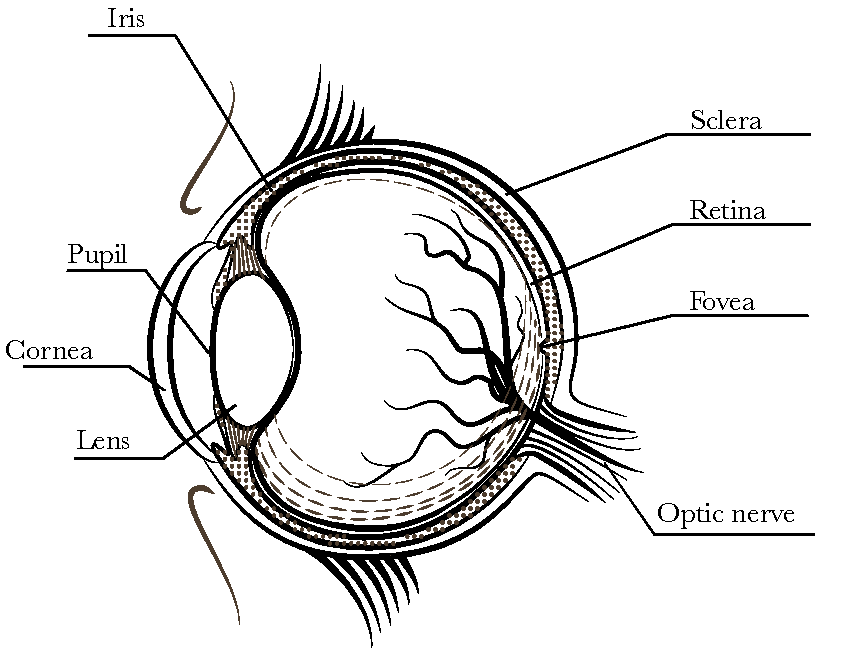
\includegraphics[width=0.8\linewidth]{figures/eye.pdf}
    \caption{Diagram of the human eye. A number of significant features have been marked. Image adapted in accordance with licence from \cite{freepik}.}
    \label{fig:anatomy}
\end{figure}

From a physiological perspective, the eye is an incredibly complex organ which reacts in variou...


\Cref{fig:anatomy} shows an overview of a human eye. It is shaped approximately like a sphere with a bulge where the \emph{cornea} is places. The most interesting areas from the perspective of eye information processes, are the retina and the frontal lens complex. 

\todo{remember references}
The \emph{retina} is a tissue covering the inside of the eye. It is composed of light sensitive neurons called photoreceptors, which react to either a wide (rods) or narrow (cones) band of light bandwidths. The rods are used for black/white vision, typically in low-light conditions due to their much higher sensitivity than cones. Cones are primarily used for colour vision as there are three types which each respond to a specific band of wavelengths. Cones have a much higher concentration around a small area on the retina called the \emph{fovea}. This area enables high visual acuity and is therefore generally considered the primary place of attention. In fact, it is well-known that, in spite of the rapid drop-off in photoreceptor density outside the fovea, the human brain succeeds in combining visual information from many individual fixations to produce what seems like high-resolution visual perception.

\begin{figure}
    \centering
    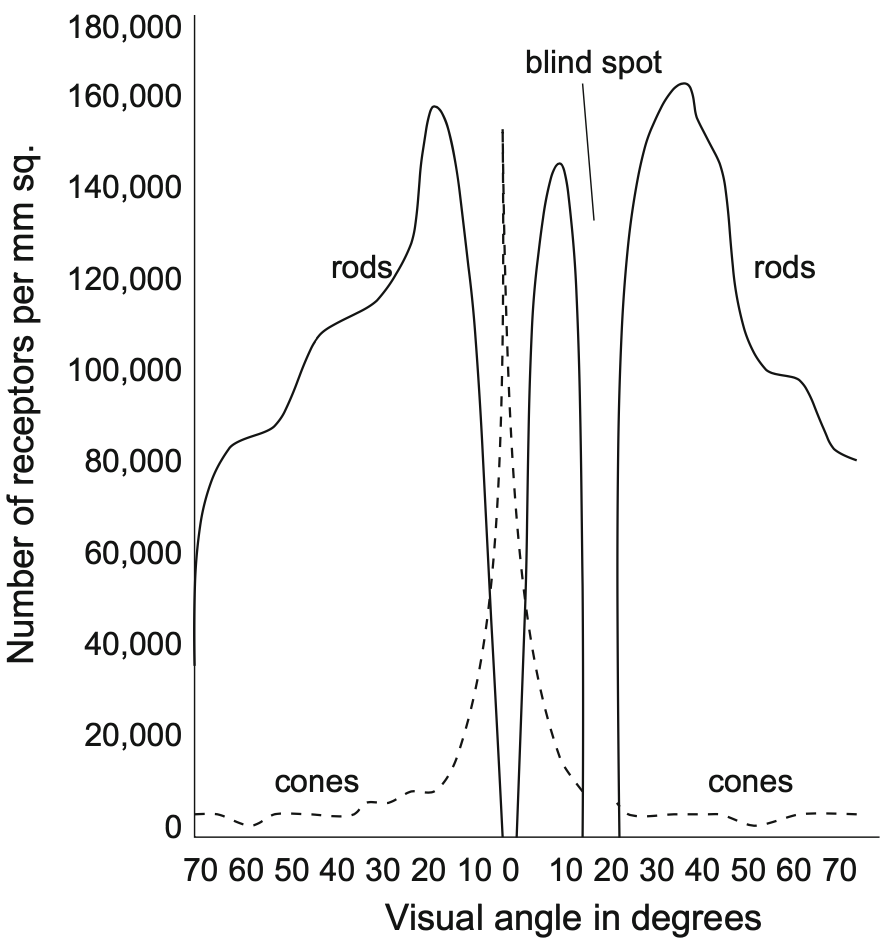
\includegraphics[width=0.6\linewidth]{figures/retina-density.png}
    \caption{Photoreceptor density as a function of visual angle (centred at the fovea). From \parencite{methodology}.}
    \label{fig:my_label}
\end{figure}

The fovea is very important for determining gaze direction or point-of-regard since it determines what is known as the \emph{visual} axis which intersects the lens centre and fovea. This visual axis typically varies slightly (about 5 degrees) from the \emph{optical axis} which intersects the cornea, pupil, and lens. This variation is different from person to person which has to be corrected by an eye-tracker. Typical modern eye-trackers have gaze direction errors of about $0.5^\circ-1.5^\circ$ which is much lower than the $\pm 5^\circ$ of the visual axis.

The frontal lens complex contains the components that allow light to enter the eye in a controlled manner. The lens system is composed of the static \emph{cornea} which accounts for a majority of the eye's optical power and the \emph{lens} which is adjusted by muscles called \emph{ciliary bodies} located behind the iris. The \emph{iris} is composed of muscles that control the size of the circular opening in its middle known as the \emph{pupil}. This allows the eye to adjust the amount of light entering the eye. 

\subsection{Eye movements}
Eye movements are formed of both conscious, semiconscious, and unconscious actions. This has led to great interest in studying these movements for various purposes, including behavioural studies as well as ...

There are five basic categories of eye movements: saccades, vergence movements, smooth pursuits, vestibular, and physiological nystagmus \parencite[39]{methodology}. Saccades are further subdivided into macro- and micro-saccades. Macro-saccades are the typical jerky movements we perform when moving from fixation to fixation. Micro-saccades are involuntary movements of $0.03-2$ degrees. The purpose of micro-saccades is to change the light-stimulus on the retina, since continuous stimulus of photoreceptors results in decreasing activation strength over time \parencite[44]{methodology}. Smooth pursuits are a mode of movement where the eye follows a fixation point on a moving object. Vergence movements are relative movements of the left and right eye to ensure vergence of the visual axes at the point of fixation \parencite{methodology}.


\section{Eye-tracking}\label{sec:eye-tracking}
\Gls{eye-tracking} covers the processes of detecting the location and movements of eyes and estimating \gls{gaze}. Gaze is defined as either a specific \acrfull{por} or as a \emph{direction}. Today, this is done exclusively through image based techniques (REF) but intrusive methods, typically using some form of special contact lens in combination with a sensor, also exist (REF).

\subsection{Why}
\begin{figure}
	\centering
	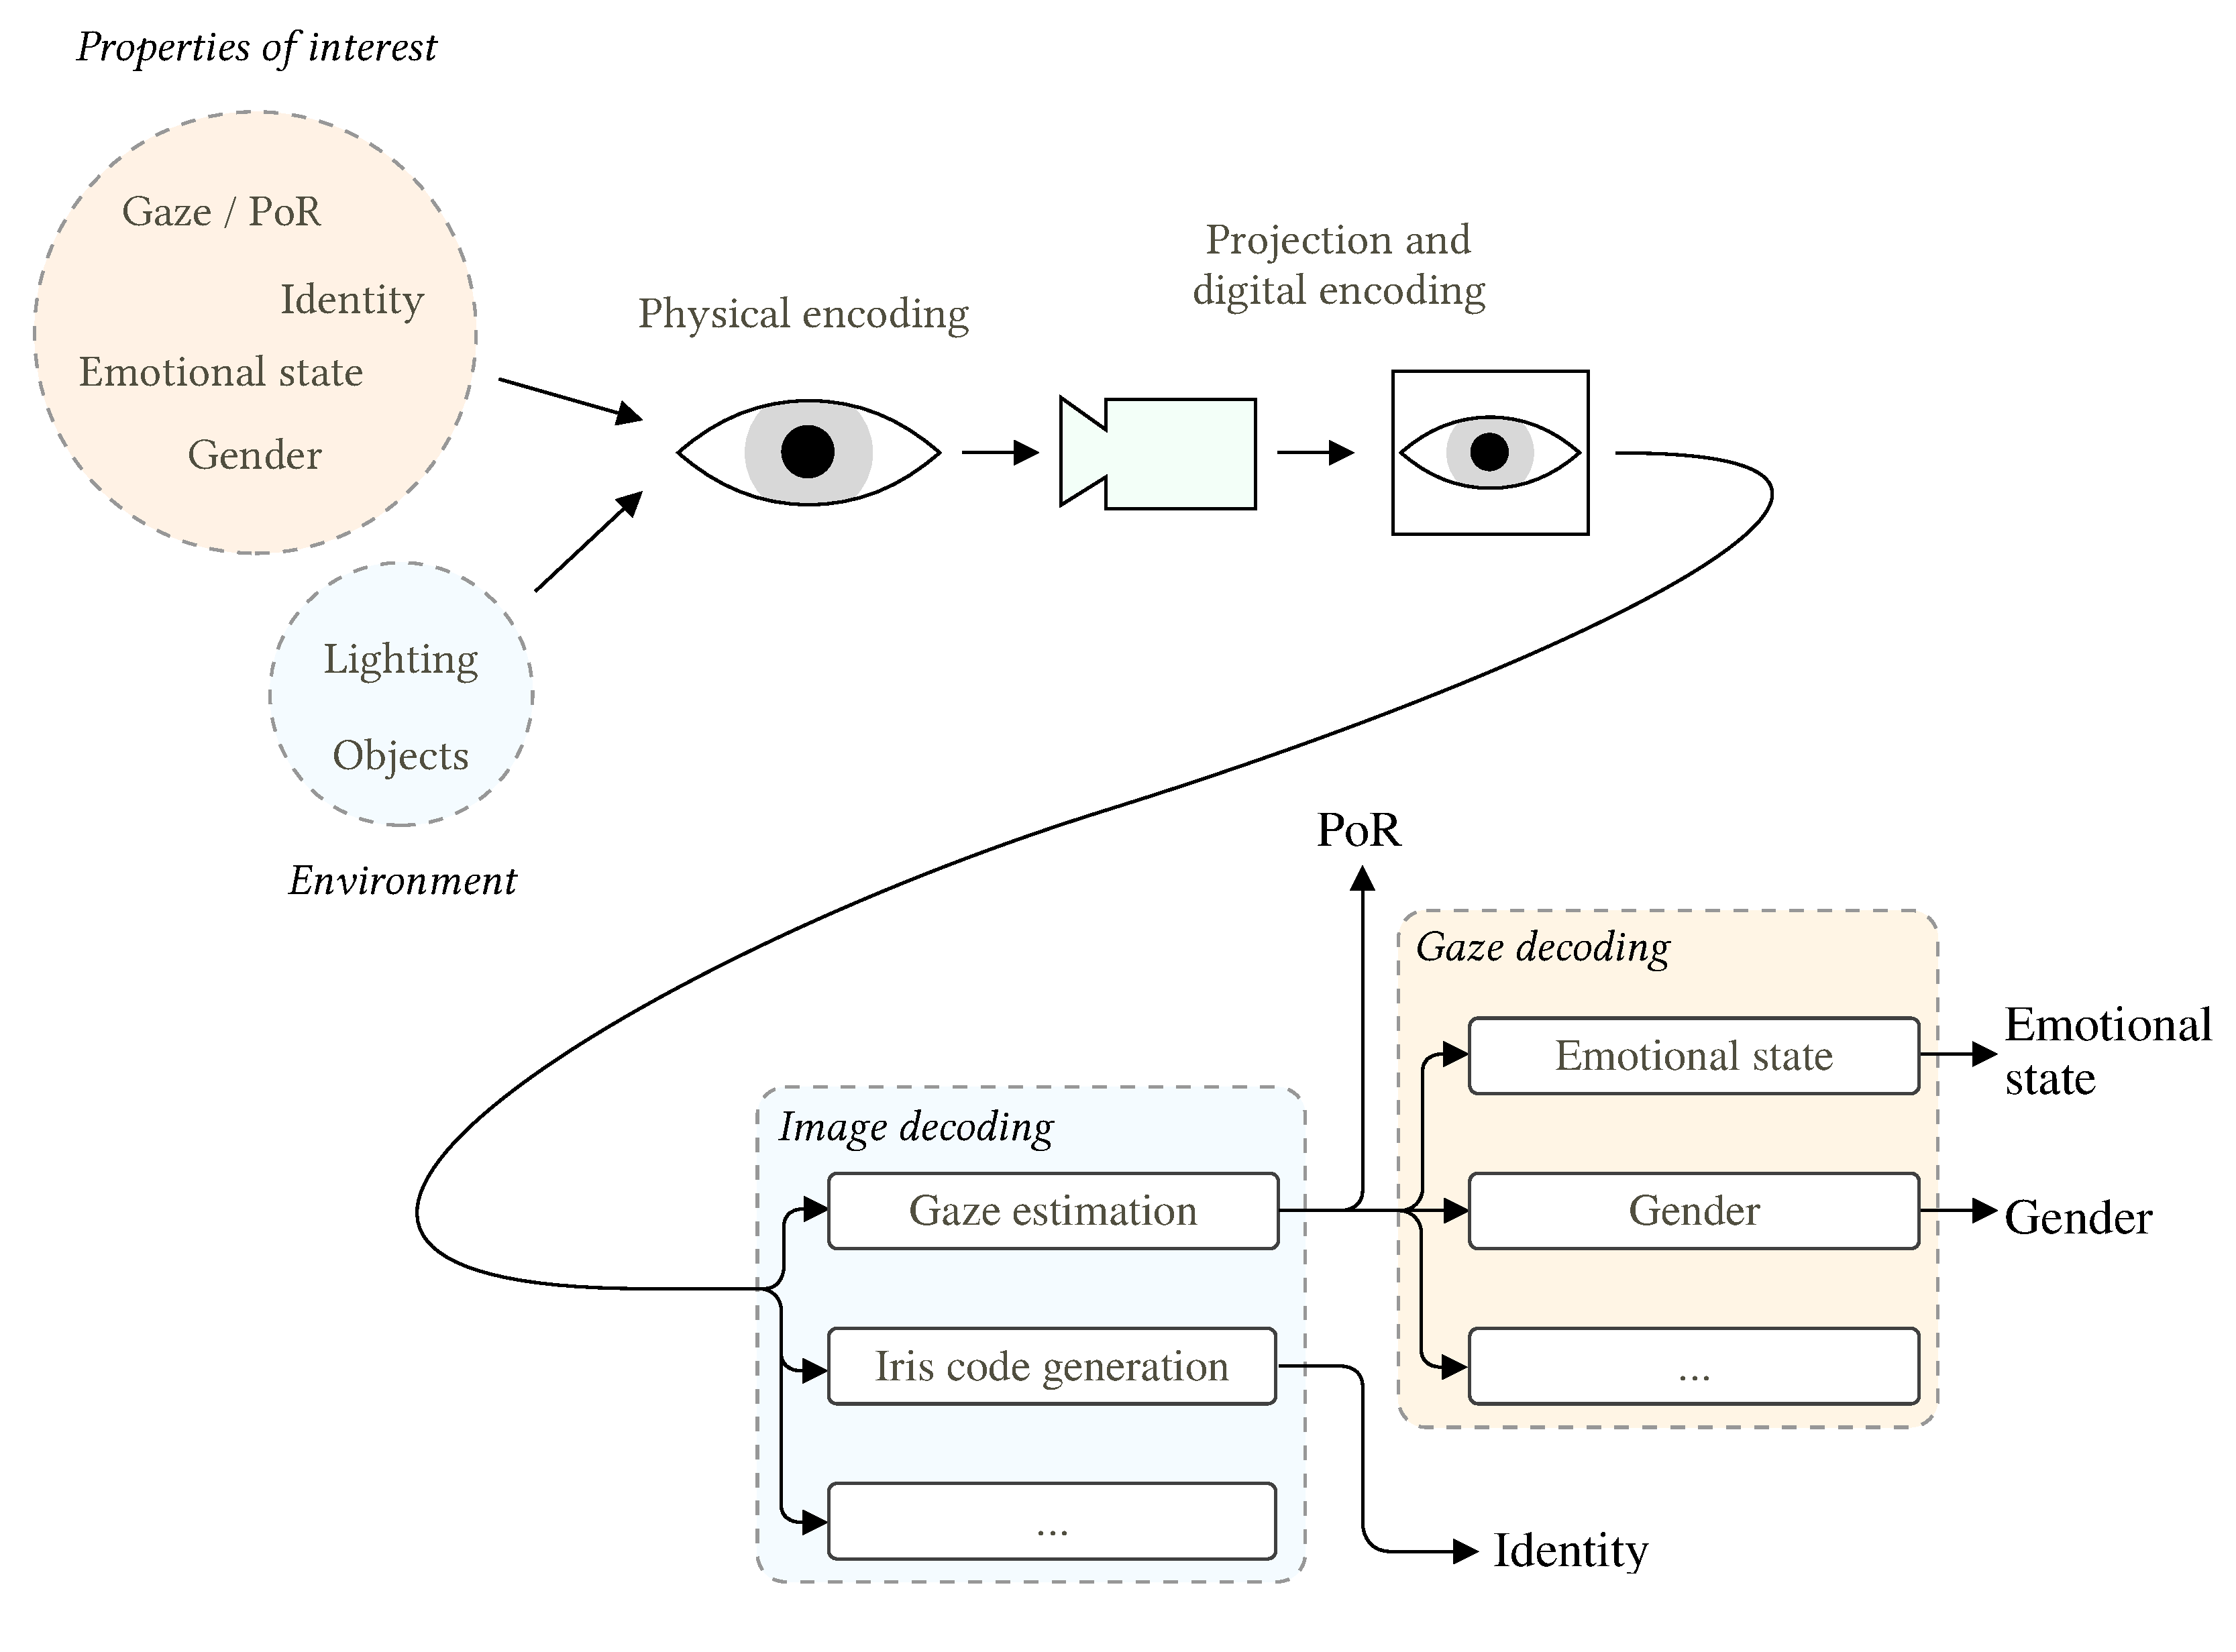
\includegraphics[width=1\textwidth]{figures/model/eye-tracking-model}
	\caption{Model overview}\label{fig:eye-tracking-model}
\end{figure}

\Cref{fig:eye-tracking-model} shows a graphical overview of an eye information processing system (EIPS). It is functionally \todo{finish this}



To understand \gls{eye-tracking}, we first need to understand the purposes for which it was made. \todo{finish}

In terms of research, \gls{eye-tracking} has traditionally been of interest in psychology (REfs) and physiology (REFS) studies due to the close connection between gaze and attention and the prominent use of eyes in humans everyday lives. A typical application is the study of visual attention, i.e. where a person is looking in a specific situation over time. Examples include studies of driver behaviour (REF), shopping behaviour (REF), analysis of reading ability and how reading works (REF), how the eyes are used in elite sports and whether analysis may be used for athletic improvements (REFS), and many more. In the medical industry, eye-tracking has been used as a tool in diagnosis of both psychological and physical conditions (REF). 

Most importantly for this thesis however, are applications in \acrfull{hci} which is a term that covers technologies or systems that act as interfaces between humans and computers (REF). The rapid decrease in part costs has made consumer-level and large-scale medical \acrlong{hci} feasible. Major corporations investing in \acrfull{vr} technologies including NVidia and Facebook, have started major research efforts towards enabling low-cost and precise eye-tracking built into \acrshort{vr}-headsets (REF). In the medical industry, technologies such as tablets have already been deployed on large scales to enrich the communication abilities of people suffering from various diseases (REF). Eye-tracking technologies that are easier to use and simpler to set up are actively being researched as well (REF). 

\subsection{How it works}
\begin{figure}
	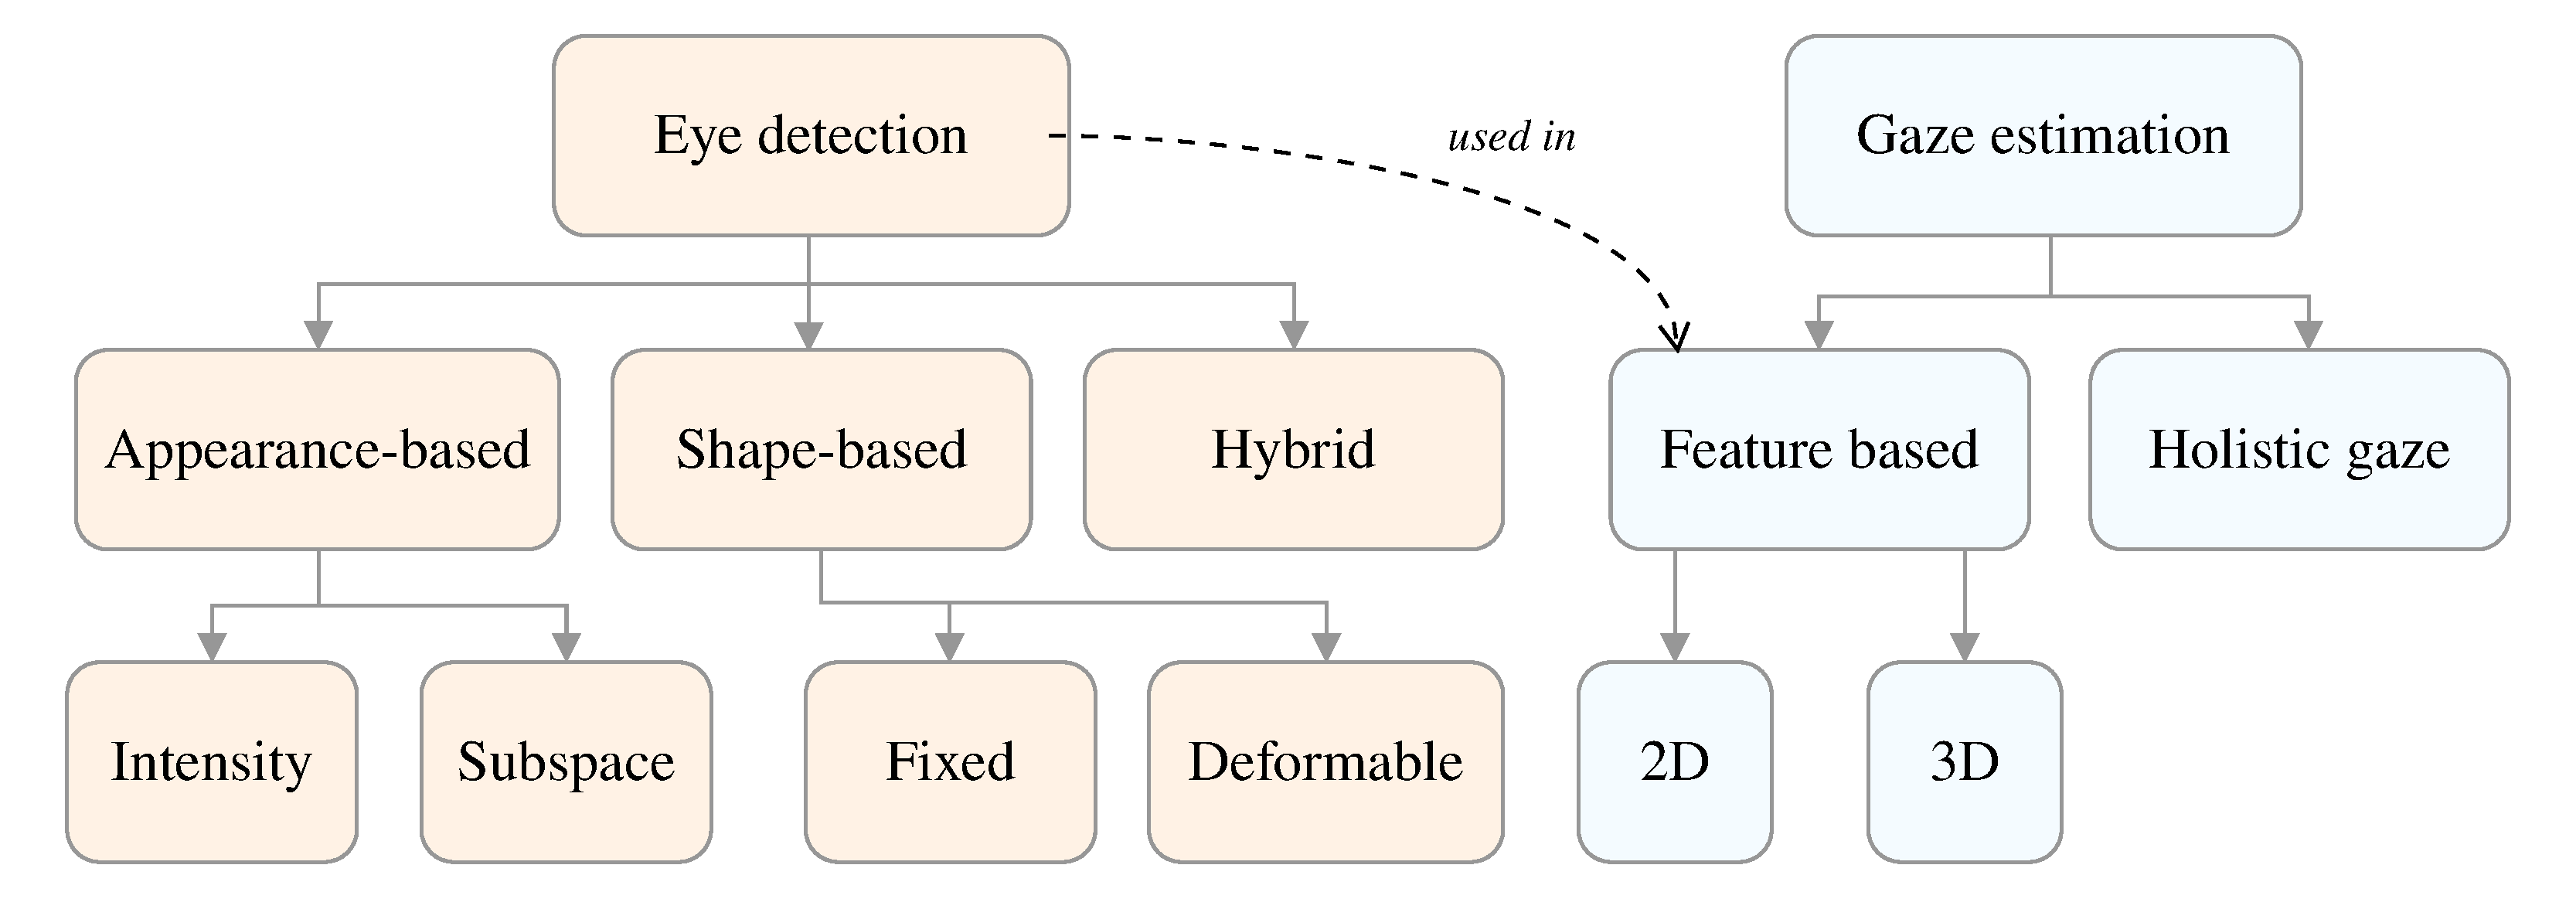
\includegraphics[width=1\textwidth]{figures/model/taxonomy}
	\caption{Eye tracking taxonomy.}\label{fig:taxonomy}
\end{figure}
All eye-tracking systems are composed of some common elements. \cref{fig:taxonomy} shows a possible component schematic of such a generalised system. At the most abstract level - an eye tracker works by capturing images of one or both of the subject's eyes and uses a number of different techniques to track the eyes themselves and to predict gaze. Because the use cases vary widely, a number of important classifications exist based on the hardware setup as well as the analysis methods employed.

The capturing setup is primarily determined by the relative mounting position of the eye-facing camera relative to the subject. In \gls{head-mounted} \gls{eye-tracking},  the eye-facing camera is fixed relative to the head of the subject and hence translational movements of the eye are kept to a minimum. The alternative is remote\todo{glossary} \gls{eye-tracking} where the camera is not fixed to the head and therefore allows more degrees of movement. Head-mounted eye-trackers may typically be augmented by a \gls{scene-camera} which points directly away from their head and can thus be used to determine what they are looking at a given point in time. \Gls{head-mounted} \gls{eye-tracker}s are often used when high-precision detection or gaze estimation is needed but comes at the cost of being less convenient to set up than a remote camera. Remote setups may provide high-precision eye-tracking if the head is fixed using a chin-rest or similar. The precision gained by fixing the relative position of eye and camera most stems mainly from the much higher utilisation of the image resolution as the eye can fill the entire image. Eye-tracking precision is generally affected by the environment, which is why controlled environments are generally preferred if possible. In many cases however, such as attention analysis, the environment cannot be controlled .... \todo{Example images and hardware setups!}

Eye-tracking systems cover a large range of use cases that require the detection of different properties. \Gls{gaze} is the most widely used end-product which may itself be used in secondary analyses of other personal properties (SECTION EYEINFO). Other important products include the iris and sclera textures which may be used for personal identification (REF) and the size of the pupil as it changes in response to external stimuli (REF). \Gls{gaze} is also typically used for eye movement analysis which produces an event-based overview of what kind of movements occur at given points in time (REFS). The different end-products have different requirements, but they all share the fundamental concept of being properties of interest that should be extracted from the source eye images. This generalisation idea is built upon in later sections (SECREF) to provide a theoretical model for eye-tracking that is useful for analysing privacy.... \todo{decide whether things should be added}

The property detection methods, of which there may be many or few in a given eye-tracking system, are typically classified as either appearance-based or feature-based. However, because of how modern systems including convolutional neural network (CNN) based ones makes the line seem less clear-cut, I redefine the two classes as holistic and local approaches after the same terms used in (dan REF). Figure (REF) shows the classification scheme. Holistic approaches consider the eye in its entirety, either by methods such as template matching (REF), or machine learning models such as CNNs mapping images directly to gaze. Local approaches instead consider specific eye elements or image features which are then combined. 

Eye-trackers may mix these methods. For example, CNNs which are inherently appearance-based have been shown to be extremely accurate at predicting the pupil centre which is then used in a two-dimensional gaze estimation model whic

\todo{Continue!}

%appearance-based and feature-based methods. The former covers methods that use the source image appearance to predict an output property

%Appearance-based methods use the image appearance itself to determine some property, e.g. eye position. This can be done either by template matching (REF), filter responses, or, more widespread today, using neural networks (REFS). 

%Feature-based 
%Shape-based models cover methods that try to fit a prior eye shape model to a single or several features in the image. Feature-based approaches aim at detecting non-typical features such as corneal reflections of LED lights or eye corners.


%Gaze estimation models are generally divided into two-dimensional models, three-dimensional models, and appearance-based models. The former two use detected eye features for gaze estimation and are therefore often collectively referred to as feature-based methods (REF dan). This is not to be confused with the feature-based paradigm itself although the two are often used together.

%The image based methods, which are the sole focus in this thesis, are typically broken down into components as shown in (FIGREF). Generally, the steps of eye detection and gaze estimation are separate, but in the case of \emph{appearance-based} gaze estimation, the image is mapped directly to gaze and thus skips the detection step. This approach is dominated by deep neural networks (REFS) and is most prominent in settings 



%Depending on the approach used, eye detection and gaze estimation may be individual steps or combined. 

%Knowing where people are looking is useful both for studying human behaviour and providing interactive technologies. 

%Eye-tracking is a scientific field that cover many different disciplines from computer science and engineering to psychology and biology. These can be divided into the research in eye-tracking technology and research enabled by eye-tracking technology. This section focuses on the former. It gives a short introduction to the eye-tracking technologies available today, how they work, and where they are used.


\section{Privacy}\todo{Needs a lot of glue and rewriting of old material}
This section presents potentially sensitive information sources in eye-tracking systems. The first part focuses on sensitive information that is extracted directly from eye images and the second part focuses on information derived from gaze signals.


Privacy is informally understood as the ability to hide information relating to your person from others. In technical terms, privacy is typically understood as the protection of information by modifying it in a way that allows only access by those who are authorised to do so. The paradox here is that the information 

 linked with probability 

 understood as the probability of ...
 
 

%\begin{displayquote}
%No one shall be subjected to arbitrary interference with his privacy, family, home or correspondence, nor to attacks upon his honour and reputation. Everyone has the right to the protection of the law against such interference or attacks.	
%\end{displayquote}


\begin{definition}[Sensitive information] 
	is any information related to a person that can be differentiated from others. This definition is a paraphrasing of the GDPR-equivalent.
\end{definition}

\begin{definition}[Privacy]
	in the context of information systems is a measure of how difficult it is to extract some property which should be hidden. 
\end{definition}


Sensitive information is thus the properties that cannot be shared freely without ethical and legal implications. Privacy is a measure of how secure a given method is at preventing that the information is shared. Encryption methods typically provide probabilistic guarantees that are so extreme that they are considered unbreakable (REF). These are however not useful in all situations.

Eye tracking data is created for the purpose of being consumed by some other process, whether it is in \acrshort{hci} or psychology. Encrypting the data, however, does not necessarily ensure protection for the user. In cases where the data is meant to be shared publicly, this is obvious by its definition. In other products, encryption only protects potential outside attackers from gaining access to the information. The producer of a given product still has the ability to use the information for various purposes and even if they don't intend to, the very presence of the information has legal implications in many areas of the world.


As mentioned briefly in (SECREF 2.1), eyes reveal many things about us. 

In this section, I outline known methods to exploit eye-tracking data for personal identification. Although iris-recognition is the most prominent method known today, other intriguing methods for identifying people based just on data on their eyes appearance or movements exist. Additionally, methods for determining a location or retrieving other personal information from e.g. scene cameras will also be presented.

\subsection{Personal identification}
Personal identification is one of the most serious privacy issues in eye-tracking since it makes it possible to link identity with other sensitive pieces of information. Using iris recognition specifically, it is possible to identity people with extremely high precision (REF). 

\subsubsection{Iris recognition}
The iris pattern in human eyes is unique and highly variable, even among twins and the left/right eye of a specific human being. It is also impossible to modify without risking damage to the eye \parencite{DAUGMAN_IRIS_ORIG}. Combined with the fact that fake eyes or lenses can be easily detected by utilising the contracting reflex of the pupil \parencite{DAUGMAN_IRIS_ORIG}, it makes the iris pattern an extremely valuable biometric. Genetics determine only the large-scale factors of the iris such as color, while the rest of its structure depends largely on initial conditions in the developing embryo \cite{kronfeldCHAPTERGrossAnatomy1962}, thus making it highly unique. 

A plethora of iris recognition methods exist. The most widely used and well-documented method is developed by John Daugman and uses Gabor wavelets \cite{daugmanHighConfidenceVisual1993} to produce a 2048-bit code for a given iris image. Identification is commenced by performing a test of statistical independence on the hamming distance between the two codes. If it fails the test, the codes are said to be a match. \autoref{fig:hamming-dist} shows the distributions of the hamming distance for similar and different irises. By adjusting the threshold for acceptance, Daugman achieves false-positive rates of as low as $10^{-13}$. This method will be used in a simplified form for the prototype presented in \autoref{sec:iris-recognition}.



In general, iris recognition methods can be categorised by their feature extraction methods. The process always starts with iris detection, segmentation, and conversion to \emph{pseudo-polar} coordinates resulting in images such as \autoref{fig:iris-code}. This raw image input is then used for extracting features that exhibit useful properties for iris identification such as lighting invariance and robustness to angle and focus.


The most common feature extraction methods are by far wavelet filter transforms \parencite{daugman2007new, ma2002iris, ma2004efficient, poursaberi2006iris, rydgren2004iris, zhu2000biometric} followed by frequency analysis techniques such as the discrete cosine transform\cite{iris-dct, monroDCTBasedIrisRecognition2007} and, more recently, deep learning based feature extractors\cite{gangwarDeepIrisNetDeepIris2016, nguyenIrisRecognitionOfftheShelf2018}.

\subsubsection{Sclera recognition}
Another measurable physical eye feature is the blood vessels in the sclera. As stated by several studies \cite{dasScleraRecognitionSurvey2013, zhouNewHumanIdentification2012}, the blood-vessels are stable over time, although the amount of literature supporting this is relatively sparse compared to iris patterns.

Methods for recognition include simple edge-filter responses with support-vector machines for classification \cite{dasNewEfficientAdaptive2014} as well as more complex processes involving the detection of individual blood vessel line segments \cite{zhouNewHumanIdentification2012}. Both methods achieve false positive rates around $10^{-2}$ for genuine acceptance rates around $80\%$.

\subsubsection{Identification based on eye movements}
Both iris and sclera recognition require relatively sharp and large eye images to be feasible. Eye movements, however, is exactly the goal of most eye-tracking systems. Of special concern is remote systems such as \cite{zhangMPIIGazeRealWorldDataset2017} that are specifically designed to track gaze based on remote camera sources such as webcams. Despite this ease of access, identification based eye movement currently suffers from some of the same problems as facial recognition, namely a much higher uncertainty and susceptibility to the recording circumstances.

Eye movement consists of multiple modes of operation. During a \emph{fixation}, the eye is relatively, but not completely, still as it focuses on a specific point. \emph{Saccades} are quick movements of the eyes and are split into macro-saccades and micro-saccades. The former describes the regular fast movement between fixations while the latter describes involuntary adjustments occurring even during fixation. \emph{Vergence shifts} describe movements to adjust binocular vision to perspective effects. Finally, \emph{smooth-persuit} movements describe the eye's ability to smoothly follow a moving object \cite{duchowskiBreadthfirstSurveyEyetracking2002}.

Identification is typically performed by comparing recorded eye movement features and testing for a statistically significant difference for rejection. Ioannis Rigas, George Economou, and Spiros Fotopoulos \cite{rigasBiometricIdentificationBased2012} present a method designed around clustering eye fixations and treating them as graphs to determine similarity. The fixations are gathered by presenting subjects with several images multiple times with the same images shown to all subjects. Other methods include feature extraction from reading scan-paths \cite{hollandBiometricIdentificationEye2011, bednarikEyeMovementsBiometric2005} and the use of Gabor filter responses to create features from scan-paths to be classified by a support vector machine\cite{liBiometricRecognitionTexture2018}. The methods all achieve much higher false acceptance rates than iris and sclera recognition methods however and it remains to be seen how effective they are in practice.

\subsection{Attribute estimation}
















\chapter{Theory}\todo{Lad det her med opdelingen simre.}
This thesis takes the perspective of viewing all eye information sources as well as their encodings as signals. This perspective is exceptionally useful when analysing uncertainty in a complex system composed of multiple information sources and with multiple goals. Additionally, it allows us to treat the objective of information obfuscation abstractly and thereby consider its use across multiple different applications. It turns out that any information extraction process can be defined in terms of just its ability to preserve the original information and be robust to noise. As a result, obfuscation methods are defined by competing goals of signal preservation for one information source (gaze) and signal degradation for another, e.g. the iris pattern. This chapter introduces and discusses the necessary prerequisites assuming a reader with knowledge of fundamental probability theory. The next chapter uses the presented theory to describe the abstract model and its implications.


%The proposed methodology and experiments rely on interpretations of eye tracking and iris recognition as communication systems of discrete signals. This requires a fundamental knowledge of information theory and signal processing which concern how uncertainty propagates and ...

%As presented in the overview, attributes such as gaze direction and personal identity can be represented as properties. These signals are encoded as physical properties which are transmitted through the medium of photons reflecting off of the eye onto a photosensitive camera sensor. This transmission creates an image, which is then processed further to ultimately decode the original properties. This is fundamentally similar to how a text message might be encoded and transmitted over a radio network to enable long distance communication.

%Information theory provides a number of tools for analysing such information transmission scenarios.
\section{Signals and information}
\begin{figure}
    \centering
    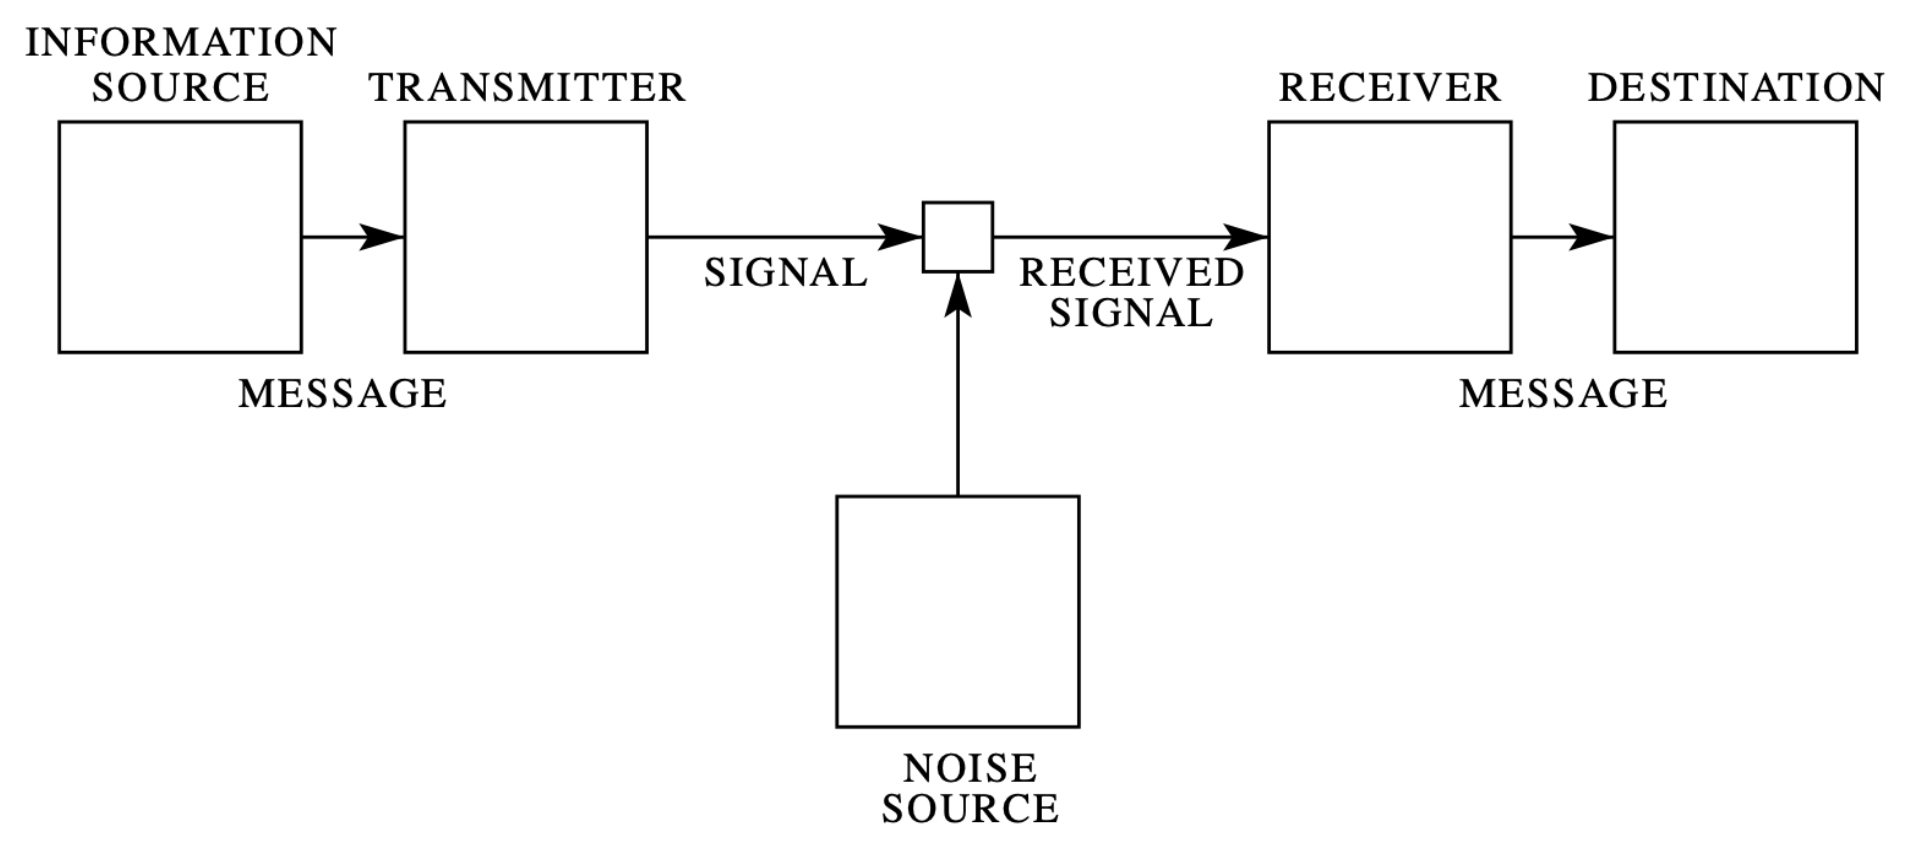
\includegraphics[width=0.8\textwidth]{figures/theory/comm-model.png}
    \caption{Diagram of communication system as depicted in \textit{A Mathematical Theory of Communication} \parencite{shannon1948mathematical}.}
    \label{fig:comm-model}
\end{figure}

\textit{Signal} is a rather vague term that is typically used to describe data that is transmitted over some medium and that contains \textit{meaningful information}. In this thesis, we use signal to denote any meaningful information that has been encoded by an arbitrary process. For example, the physical position and rotation of the eye is an encoding of several properties including point of regard. Information theory is a theoretical framework introduced by Claude Shannon for precisely measuring uncertainty in communication systems \parencite{shannon1948mathematical}. The signals of interest in case of eye-tracking and obfuscation methods are either images or time-based signals such as gaze or eye-feature parameters. These signals are only observed in discrete intervals defining units of time, space, or both. We therefore only consider the discrete parts of information theory. 

As shown in \cref{fig:comm-model}, a communication system consists of an information source that is transmitted as a signal over a channel and then decoded back into its original representation. This basic diagram can be applied to many kinds of situations including error handling, compression, and, as proposed in this thesis, eye information obfuscation.


Information theory defines entropy as a measure of uncertainty. It is a logarithmic function of the randomness of the transmitted signal. 
The base measure is entropy, denoted $H$ which defines the optimal average encoding length of symbols $x_i$ drawn from a discrete distribution $X$ defined by
\todo{Alt herunder skal revideres med flere detaljer + mere historiefortælling}
\begin{definition}[Shannon entropy]
The Shannon entropy is the expectation of the self information $I(X)$ of each outcome of $X$:
\begin{equation}
    H(x) = \mathbb{E}[h_X(X)] = - \sum_i p_i\log p_i
\end{equation}
\end{definition}

with results in the units of bits. Different bases may be used for alternate units. A uniformly distributed discrete random variable has an entropy of $\log{N}$ which is maximal for its number of states. Analogous to conditional probability, the notion of conditional entropy signifies the entropy of a signal given knowledge of another. In \cref{fig:comm-model}, the conditional entropy can only originate from the noise source but in general, any number of signals may be combined in a channel and affect the conditional entropy. It can be defined in terms of the distributions of input and output signals $X$, $Y$.

%In terms of iris recognition, the entropy of code symbols (bits are typically used) can be used to calculate the expected amount of information present in the entire signal. 

%For example, Daugman calculated the expected iris code entropy by fitting a binomial distribution to the iris code distance comparisons, which revealed an approximate 250 bits of information between codes (REF). This entropy only accounts for the information content in the final codes and thus does not account for noise added during the encoding and processing steps. 



\begin{definition}[Conditional entropy]
For random variables $X$, $Y$, the conditional entropy $H(Y|X)$ is defined by:
\begin{equation}
    H(Y|X) = \sum_{x\in\mathcal{X}, y\in\mathcal{Y}} p(x, y)\log\frac{p(x, y)}{p(x)}
\end{equation}.
\end{definition}

When a signal is transmitted over a channel, the mutual information defines the amount of uncertainty in the channel output that originates from the original signal. This measure is thus limited by the entropy of the source signal.

\begin{definition}[Mutual information]
The Shannon entropy is the expectation of the self information $I(X)$ of each outcome of $X$:
\begin{equation}
    I(Y;X) = \sum_{x\in\mathcal{X}, y\in\mathcal{Y}} p(x, y)\log\frac{p(x, y)}{p(x)p(y)}
\end{equation}
\end{definition}

The entropy of input and output signals $X$, $Y$ is related by how much information is shared between them (mutual information) and how much is introduced by the channel (conditional information). \cref{fig:entropy-comp} visualises this relationship which is written as
%The signal entropy over a channel can be decomposed into exactly the entropy carried over from the original signal (mutual information) and the noise introduced by the channel itself (conditional information) as shown visually in \cref{fig:entropy-comp}. This is encoded in the following relationship
\begin{align}\label{eq:entropy-law}
    H(X) = I(X;Y)+H(X|Y).
\end{align}

This is easily derived from the definitions of mutual information and conditional information
\begin{align*}
    I(X;Y)+H(X|Y) &= \sum_{x\in\mathcal{X}, y\in\mathcal{Y}} p(x, y)\log\frac{p(x,y)}{p(x)p(y)} + \left(-\sum_{x\in\mathcal{X}, y\in\mathcal{Y}} p(x, y)\log\frac{p(x,y)}{p(y)} \right) \\
    &= \sum_{x\in\mathcal{X}, y\in\mathcal{Y}} p(x,y)\left(\log{p(x,y)}-\log{p(x)}-\log{p(y)}-\log{p(x,y)}-\log{p(y)}\right)\\
    &= \sum_{x\in\mathcal{X}, y\in\mathcal{Y}} p(x,y)\log\frac{1}{p(x)}\\
    &= - \sum_{x\in\mathcal{X}} p(x)\log{p(x)}\\
    &= H(X).
\end{align*}

\begin{figure}
	\centering
	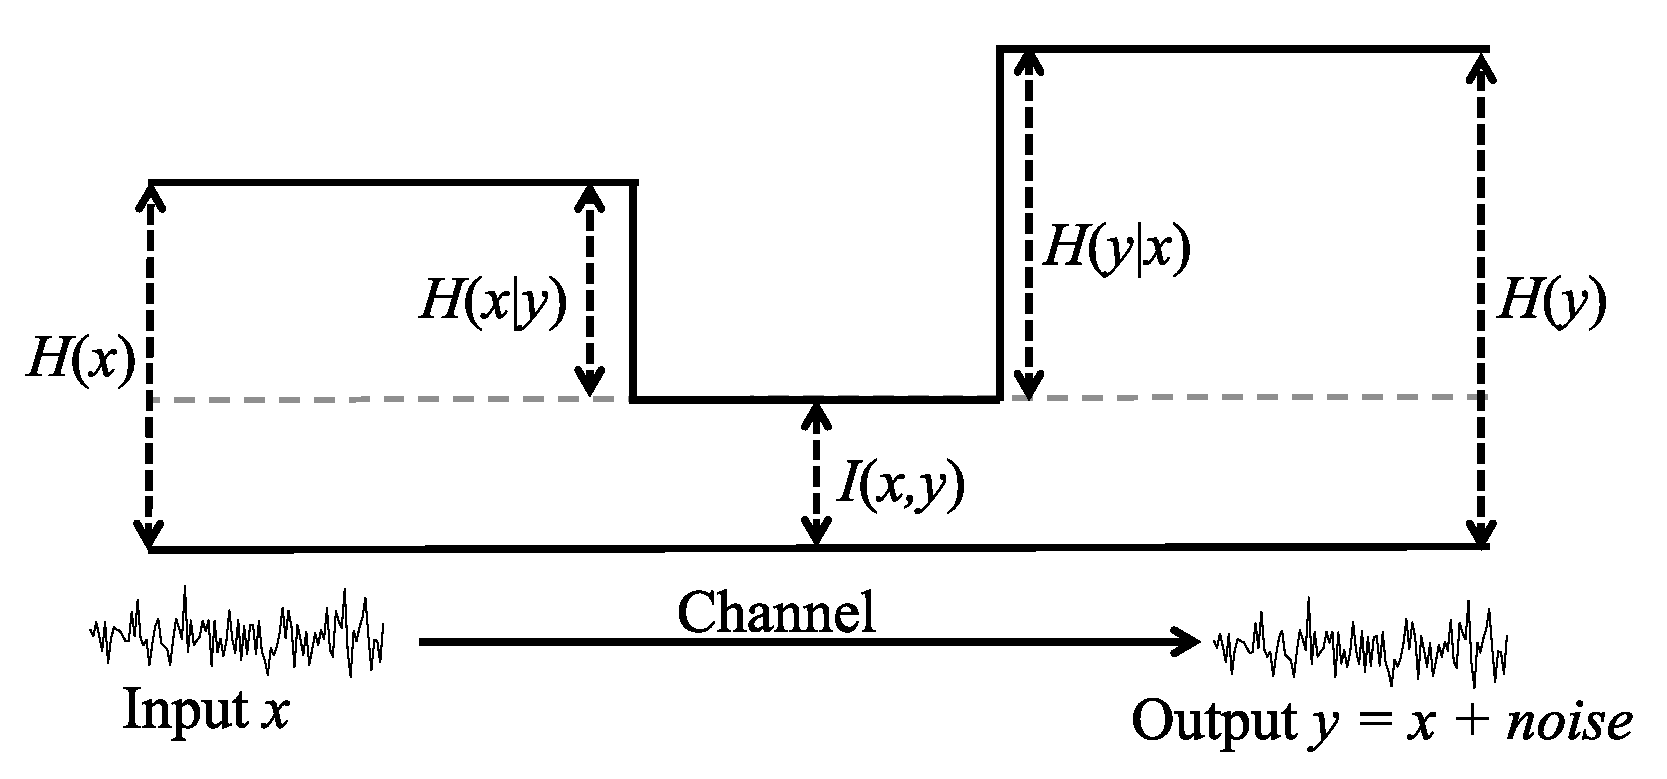
\includegraphics[width=0.8\textwidth]{figures/theory/entropy-comp}
	\caption{Hej}\label{fig:entropy-comp}
\end{figure}





%For iris obfuscation, the goal is to minimise $I(R_{iris}, Q_{iris})$ and maximise $I(R_{gaze}, Q_{gaze})$. Measuring these directly is again not possible as the $Q$ signals are not the measured signals. The only known information source is the image $I$ where the two signals have been combined into a single signal. However, because $H(Q_{gaze})$ should be very low, i.e. it represents an encoding of just two real values, the mutual information between the original and obfuscated images $I(I, I^*)$ can be used as a proxy to measure the level of obfuscation. Additionally, for any set of signals $X, Y, Z$ where $Z = f_z(Y)$ and $Y= f_z(X)$, then $I(Z; Y) \leq I(Z;X)$ (REF to proof). Thus, it is an upper bound for the mutual information which makes the results much more useful.

Finally, the notion of channel capacity is used to define the maximum mutual information of a channel for any input distribution. It is defined as
\begin{align}
    C = \max_{p_x} I(X, Y).
\end{align}
The channel capacity of specific obfuscation methods define strong upper limits on the amount of information that is able to pass. If an obfuscation method has capacity below the minimum requirement for differentiation of a population given the optimal distribution (uniform), it is impossible to accurately differentiate between all individuals. In practice, however, the image signal which is measured contains orders of magnitude more information, making such guarantees unlikely, at least for the methods presented in this paper. Instead, we use the measure to evaluate the relative obfuscation of information.

%%%%%%%%%%%%%%%%%%%
% Extra stuff - unlikely to get time to fix
%%%%%%%%%%%%%%%%%%%

%\subsection{Properties of mutual information}
%Mutual information can be generalised to multivariate cases. In ...

%\begin{definition}
%Given a set of $n$ random variables $X$, the mutual information between any subset $S\subset X$ is less than the mutual information of the whole set, i.e.
%\begin{equation}
%     I(S) \leq I(X)
%\end{equation}
%\end{definition}

%proof: By the definition of measures, the mutual information $I$ is always non-negative, i.e. $I > 0$. Since $I(X) = I(X^1, \dots, X^{n-1}) - I(xxx)$, $I(X^1, \dots, X^{n-1}) \leq I(X)$.

%%%%%%%%%%%%%%%%%%%

% \section{Information theory}
% Uncertainty is similar to electrical voltage in that it represents a relative difference between knowledge and the lack thereof. Information is a measure of change in uncertainty over time. In other words, a highly uncertain message will impart the receiver with a large amount of information on arrival. If the receiver already knows part of the message, they will be less uncertain of its contents and therefore receive less information on arrival. 

% Information theory is a mathematical field which defines a useful theoretical model for information along with a large body of work In essence, information theory uses the language of probability and measures to define and quantify uncertainty of the signals and transmission procedures.



% Information represents the gap between not knowing and knowing and is thus inherently relative. It is similar to electrical voltage in that 

% The fact that information is a measure of uncertainty might seem counter intuitive when it feels like information should be the lack of uncertainty. This is, not surprisingly, the result of a misunderstanding. Information is not the randomness itself, but instead represents the amount of uncertainty removed when a random variable is observed.

% \begin{definition}[Self information]
% \begin{equation}
%     h_x(x) = -log(p_x(x))
% \end{equation}
% \end{definition}

% \begin{definition}[Shannon entropy]
% The Shannon entropy is the expectation of the self information $I(X)$ of each outcome of $X$:
% \begin{equation}
%     H(x) = \mathbb{E}[h_X(X)] = - \sum_i p_i\log p_i
% \end{equation}
% \end{definition}

% \begin{definition}[Joint entropy]
% The Shannon entropy is the expectation of the self information $I(X)$ of each outcome of $X$:\todo{Detailed description - shorten notation and provide explanations}
% \begin{multline}
%     H(X^1, \dots, X^n) = -\mathbb{E}[h_X(X^1, \dots, X^n)] =\\ - \sum_{x^1\in\mathcal{X^1}} \dots \sum_{x^n\in\mathcal{X^n}} p_{X^1, \dots, X^n}(x^1, \dots, x^n)\log p_{X^1, \dots, X^n}(x^1, \dots, x^n)
% \end{multline}
% \end{definition}

% \begin{definition}[Conditional entropy]
% The Shannon entropy is the expectation of the self information $I(X)$ of each outcome of $X$:
% \begin{equation}
%     H(Y|X) = \sum_{x\in\mathcal{X}, y\in\mathcal{Y}} p(x, y)\log\frac{p(x, y)}{p(x)}
% \end{equation}
% \end{definition}

% \begin{definition}[Mutual information]
% The Shannon entropy is the expectation of the self information $I(X)$ of each outcome of $X$:
% \begin{equation}
%     I(Y;X) = \sum_{x\in\mathcal{X}, y\in\mathcal{Y}} p(x, y)\log\frac{p(x, y)}{p(x)p(y)}
% \end{equation}
% \end{definition}

% \begin{equation}
%     H(X) = H(X|Y) + I(X;Y)
% \end{equation}

% \begin{definition}[KL divergence]
% The Shannon entropy is the expectation of the self information $I(X)$ of each outcome of $X$:
% \begin{equation}
%     D_{KL}(P||Q) = \sum_{x\in\mathcal{X}}p(x)\log\frac{p(x)}{q(x)}
% \end{equation}
% \end{definition}

% \begin{align}
%     I(Y; X) = D_{KL}(p_{x,y}||p_x\times p_y)
% \end{align}

% \chapter{Information and signals}
% This chapter reviews the theoretical tools used for the modelling and analysing eye information in this thesis. It is an expanded version of the presentation in the article and reveals more details of how the theoretical parts connect and have directly inspired the solution proposals.



\section{Signal processing}
This section introduces a number of central concepts of signal processing that are used throughout the thesis in both the model proposal, experiments, and evaluation. Signal processing is widely used in computer vision and is equally applicable for one-dimensional time-series data such as gaze signals. The signals of interest in case of eye-tracking and obfuscation methods are either images or time-based signals such as gaze or eye-feature parameters. These signals are only observed in discrete intervals defining units of time, space, or both. 

The field of signal processing generally concerns signals that are at least approximately continuous. The reason is that many real-world phenomena when measured resemble continuous functions. More specifically, signal processing concerns how to characterise and transform signals measured at discrete intervals using frequency analysis.  



In its most abstract form, a signal is simply a function. Typically though, signals are used specifically to refer to functions that are representations of a physical or abstract quantity that varies in intensity over its range. \emph{Signal processing} is a scientific field covering the study of signals. This includes analysis 

\subsection{Fourier analysis}
Fourier analysis uses sinusoidal functions to analyse the presence of cyclic elements in functions. It is based on the observation that functions can generally be approximated by a sum of complex exponentials (complex sinusoids). This sum is called a Fourier series and has the following definition:
\begin{equation}
    s_N(x) = \sum_{n=-\infty}^{\infty} c_n \cdot e^{i\frac{2\pi n x}{P}},
\end{equation}
where $c_n$ are the Fourier coefficients (weights) of each exponential. A Fourier series requires the target function $f: A \rightarrow B$ to be periodic, i.e. $\forall x\in A: f(x+P) = f(x)$ for some $P\in A$.

The Fourier Transform, or rather its inverse, is a generalisation of the concept of approximating functions using sums of complex sinusoids which does not require the source function to be periodic. The regular Fourier Transform allows decomposition of an arbitrary function into its frequency constituents. It is an integral transform defined as

\begin{align}\label{eq:conv}
	\hat{f}(\xi) = \int_{-\infty}^{\infty} f(x) e^{-2\pi i x\xi}dx,
\end{align}
where $\xi$ is a given frequency. For example, the Fourier transform of a \todo{example function}. The complex exponential $e^{-2\pi i x\xi}$ is by definition periodic (\todo{example image}) and as such the Fourier transform can be understood as measuring the degree to which the origin function responds to a specific period. The Fourier Transform is a powerful tool that allows decomposition of functions into their frequency components. 

Frequency analysis is used in this thesis as a tool for understanding how various processes affect images and how the iris pattern and features used for gaze estimation are represented in the frequency domain.

\subsection{Image filters}
This section introduces the notion of convolution since it is essential to understanding how the presented obfuscation methods interact with the eye images and how information is extracted from the images to estimate gaze and produce iris codes.

Convolution, denoted by the symbol $*$, is an operation on two functions that use one function as a sliding template. In the continuous domain, convolution is defined as
\begin{equation}
    (f*g)(t) = \int_{-\infty}^\infty f(\tau)g(t-\tau)d_\tau
\end{equation},
for functions $f$ and $g$. 
What the convolution operation actually does, is best explained by looking at its Fourier transformation. In the frequency domain, a convolution is simply the multiplication of the Fourier transformation of the source functions, i.e.
\begin{equation}
    \widehat{(f*g)}(t) = k\hat{f}(t)\hat{g}(t),
\end{equation}
where $k$ is a constant that depends on the normalisation of the Fourier transform. This is known as the \emph{convolution theorem}. Thus, a convolution is really a multiplication of the frequency components of the source functions. This has the implication that convolutions inherently modify specific frequencies, making them ideal candidates for implementing band-pass filters. 

For images, convolution is expressed in the spatial domain as
\begin{align}
    \hat{I}(x, y) = \sum_{i=x-s}^{x+s}\sum_{j=y-s}^{y+s} I(x,y)k(i,j),
\end{align}
where $I$ is an image and $k$ is the modifying function (a.k.a. convolution kernel) and both are represented by matrices. $s=w/2 -1$ where $w$ is the width of $k$.
\todo{introduce gabor filter banks and figures!}




\subsection{Localising frequency}
\begin{figure}
\begin{subfigure}{0.49\textwidth}
	\centering
	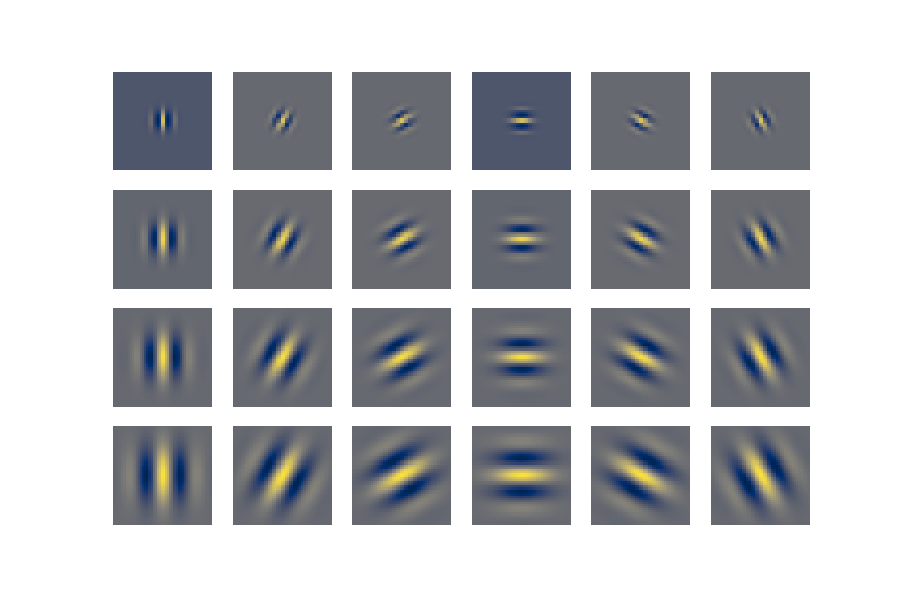
\includegraphics[width=1\textwidth]{figures/theory/gabor_sample}
	\caption{Spatial domain}
\end{subfigure}
\begin{subfigure}{0.49\textwidth}
	\centering
	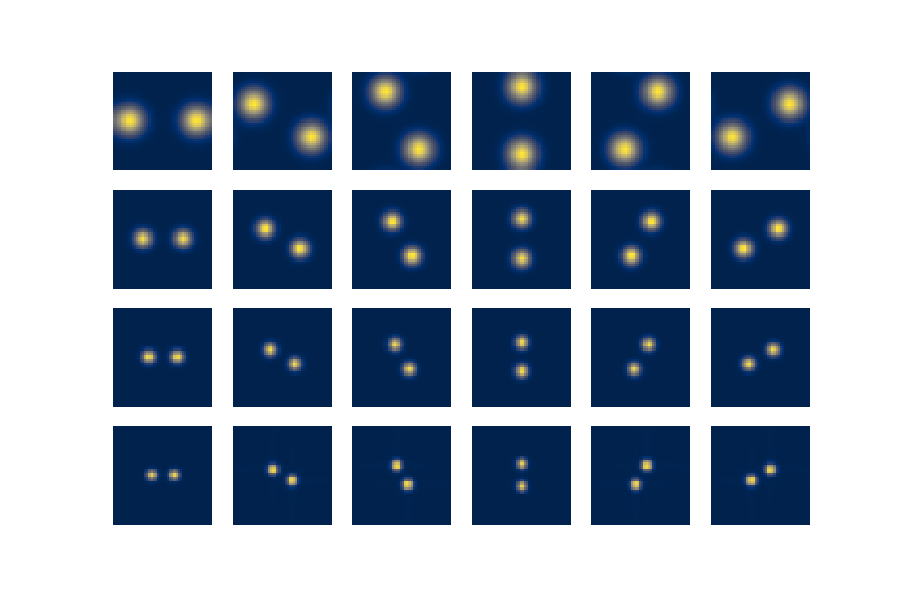
\includegraphics[width=1\textwidth]{figures/theory/gabor_sample_f}
	\caption{Frequency domain (amplitude)}
\end{subfigure}
\caption{Sample Gabor filter bank in both spatial (left) and frequency domain (right).}\label{fig:gabor-sample}
\end{figure}

The Fourier Transform is not localised and therefore does not reveal any spatial understanding of how frequencies are distributed in a given function. Knowing this is, however, extremely useful in image analysis. Spatially localised frequency analysis is the basis of edge and blob detection in images and is also used in feature-detection and texture analysis applications such as iris recognition. Several approaches exist to localise frequency responses but the most important method, and the one relevant to this thesis for both iris recognition and analysis of iris obfuscation, is the wavelet transform.

The wavelet transform is, just as the Fourier Transform, an invertible transform but instead of complex exponentials which have infinite support, it uses a wavelet function which has local support, i.e. it is only non-zero for some finite area around the origin. It uses an orthonormal series of wavelets to decompose the original signal into a number of frequency-bands.

As suggested by the treatment of convolutions, wavelet transformations for a single frequency-band can be implemented using the convolution operation. Many wavelet types exist, but in this thesis only the Gabor wavelet is used.


%This is clear when they are viewed in the Fourier domain (FIGREF). Compared to the Gaussian filter (left) and the high-pass filter (right), the wavelet filter (Gabor function) is ....

A Gabor wavelet is simply the product of a complex sinusoidal function (also called complex exponentials) and a complex Gaussian function. Here, we define it in a two-dimensional variation with adjustable frequency $\omega$, angle $\theta$, and standard deviation $\sigma$ of the envelope:
\begin{align}
    g(x,y)_{\omega, \theta, \sigma} &= \frac{1}{\sigma\sqrt{\pi}} e^{-\frac{\hat{x}^2+\hat{y}^2}{2\sigma^2}} e^{i 2\pi \hat{x}\omega}\\
    \hat{x} &= x\cos\theta + y\sin\theta \\
    \hat{y} &= -x\sin\theta + y\cos\theta.
\end{align}

\todo{wavelet example}


























%\section{Image entropy}\todo{Omskriv og tilføj detaljer}
%Entropy is based on a representation of signals as random samples, at least in the discrete case which is the one we consider here. This means that individual symbols are independent by the definition of a random sample (REF). Consequently, signals that exhibit clear correlations between symbols are not accurately presented. By definition of mutual information $H(Y|X) \leq H(Y)$ with equality achieved only if they are independent, i.e. $I(X;Y) = 0$. 

%Image pixels are not typically independent, as the light measurements they represent are highly dependent on the scene in which it was taken. A pessimistic view is that none of the pixels are completely independent of each other. In this case, the entropy of an image $I$ 

%I therefore proposal a general notion of creating a transformation of $I$ such that its individual symbols become independent. 

%The image gradient, denoted $\nabla I$ ...

%Gabor wavelet filters 

%In order to calculate the mutual information between the original and filtered images, it is necessary to create their joint distribution as well. Since both the gradient and frequency response distributions are two-dimensional, the joint distribution is four-dimensional

%\begin{multline}
%    P_{f_x, f_y, \hat{f}_x, \hat{f}_y}(x, y, \hat{x}, \hat{y}) = \sum_m\sum_n \delta_{i, f_x(m, n)}\delta_{i, f_y(m, n)}\delta_{i, \hat{f}_{\hat{x}}(m, n)}\delta_{i, \hat{f}_{\hat{y}}(m, n)}
%\end{multline}

%The rather cumbersome expression for the mutual information is
%\begin{multline}
%    I(f, \hat{f}) = \sum P_{f_x, f_y, \hat{f}_x, \hat{f}_y}(x, y, \hat{x}, \hat{y}) \log \frac{P_{f_x, f_y, \hat{f}_x, \hat{f}_y}(x, y, \hat{x}, \hat{y})}{P_{f_x, f_y}(x, y)P_{\hat{f}_x, \hat{f}_y}(\hat{x}, \hat{y})}
%\end{multline}

%Clearly, photographs are an example of signals where each symbol is highly dependent on the others because they represent measurements of light which is dependent on the physical location. ...

%This is not a property of the image format itself, perfectly random and independent pixel values can easily be created synthetically, but of the physical world. Images are nothing more than a series of measurements of light intensity. The light intensity however, is dependent on the objects and materials that has emitted or affected it. Since physical objects 

%\begin{equation}
%    H(X, Y) = 
%\end{equation}











\chapter{A model for eye information}
This chapter introduces a model for understanding and working with eye information processing systems. It is meant both as an abstract model for easily understanding the components of eye information systems and their interconnections and as a mathematical model which allows analysis of methods for information extraction and information obfuscation. The driving idea behind this approach is discovering connections between applications and being able to apply results from other adjacent scientific fields to eye information problems. Thus it is an attempt at answering the questions of how information can be quantified in a way that does not depend on specific use cases or algorithmic implementations. This leads to two things: (1) It drives the process of discovering and analysing the mechanisms by which the properties are communicated towards general concepts that provide insight into privacy in general. (2) It can, by design, lead to the creation of metrics which are usable in optimisation-based methods and thus enable data-driven method discovery.

The experimental work conducted as part of this thesis is centred around iris obfuscation. Iris obfuscation is interesting because iris recognition is well-studied and highly accurate. The model presented here is created for general use in obfuscation but is inspired by the experimental work performed as part of this thesis.

\section{Eye information processing systems}
An EIP system is the term used in this thesis to denote a generalisation of eye-tracking systems that includes any hardware/software system that decodes human properties using the eye as a source. 

\begin{definition}[Eye information processing (EIP)]
	EIP denotes a generalisation of the methods used in eye-tracking and other systems using eyes as a source of information. 
\end{definition}

\Cref{fig:eye-tracking-model} shows a simple graphical representation of the components of such a system. It includes a number of example properties, with some being decoded from the gaze signal instead of the eye images directly. This graphical representation contains the eye-tracking systems mentioned in \cref{sec:eye-tracking} as well as other systems such as iris-recognition. Sometimes iris-recognition may be seen as part of eye-tracking due to its typical use of eye-tracking techniques to find the iris but defining a separate term, eye information processing system, stresses the importance of the generalisability of the model.

EIPs closely resemble the communication model presented in \cref{sec:comm}. The properties of interest affect the physical world which acts as an encoding of a message, where the message is the properties. In communication systems, multiple messages, i.e. properties in EIP systems, may be encoded into a single signal. 

%Of course, the state of the world and even a human's eye does not only depend on a few properties which is why the encoding is both extremely complex and likely seems noisy due to other properties such as lighting that affect the state of the world. 

Viewing the world as an encoded signal might seem needlessly abstract but it is only conceptually important for the model, i.e. we expect the state of the world to be unknowable without observation. Therefore, only the signal captured by the instrument of observation, which in this case is a camera, is of interest. A camera works by measuring photons over a time interval at a large number of typically equally spaced locations. Since the light intensity is only measured at discrete locations, the resulting image signal is discrete as well. 

The process of image capture can be viewed as a channel transmission. Similarly to a channel, a camera introduces noise due to optical and sensor limitations and has a limited capacity. The actual capacity of an image depends on the model assumed for the interdependence of individual pixels but is $H(X)\times W\times H$ bits if independence and zero noise is assumed, where $H(X)$ is the entropy of a single pixel and $W$, $H$, is the width and height of the image respectively. Additional image processing steps may be seen as additional channels. This idea is essential to the concept of obfuscating information since it uses channel coding theory to describe how it works. 

Finally, the eye-detection, gaze-estimation, iris code generation, and all other products of EIPS work as decoders, i.e. their purpose is to recreate the original property. From this perspective, all operations in between the property encoding and decoding, including image capture and all image processing steps, may be viewed as a single channel. Additionally, the properties themselves may be viewed as signals, e.g. an iris code is a signal that represents a certain individual and a gaze signal represents their eye movements over time. This means that the communication model can be applied over different parts of EIPS depending on the situation. The next section presents a formulation using a graphical model to generalise this concept.


\section{Formal model}
\begin{figure}
\centering
\begin{tikzpicture}[node distance=1.5cm]
    	\node (qg) [circ] {$Q^{gaze}$};
    	\node (inv) [right of=qg] {};
    	\node (qi) [circ, right of=inv] {$Q^{iris}$};
    	
    	\node (ce) [circ, below of=inv] {$I$};
    	\node (co) [circ, below of=ce] {$I^*$};
    	
    	\node (binv) [below of=co] {};
    	\node (qbg) [circ, left of=binv] {$\bar{Q}^{gaze}$};
    	\node (qbi) [circ, right of=binv] {$\bar{Q}^{iris}$};
    	
    	\draw [arrow] (qg) -- node[anchor=south west] {$f_{enc}$} (ce);
    	\draw [arrow] (qi) -- (ce);
    	\draw [arrow] (ce) -- node[anchor=east] {$f_{obf}$} (co);
    	\draw [arrow] (co) -- node[anchor=south east] {$f_{gaze}$} (qbg);
    	\draw [arrow] (co) -- node[anchor=south west] {$f_{iris}$}(qbi);
\end{tikzpicture}
    
\caption{EIP model for iris obfuscation. $Q^{gaze}$, $Q^{iris}$ are the signals of interest encoded and captured through $f_{enc}$ in the image signal $I$. The obfuscation function $f_{obf}$ produces a modified signal $I^*$ which is then decoded by a gaze estimation system $f_{gaze}$ and an iris code generator $f_{iris}$.}
\label{fig:model}
\end{figure}

%We define a model that allows easy analysis from both a signal-processing centric and probability centric view. 
This section describes a graphical model that incorporates the concept of understanding EIP as communication and presents analyses of gaze-estimation, iris-recognition, and gaze property extraction using the model.

%An eye information processing system is defined by a connected, directed acyclic graph with vertices $V=\{\mathcal{E}, \mathcal{C}, \mathcal{D}\}$ describing random variables structured as a set of encoding processes $\mathcal{E}_1, \dots, \mathcal{E}_e^n$ and a set of decoding processes $\mathcal{D}_1, \dots, \mathcal{D}_n$ connected by a single common channel $\mathcal{C}$. Edges $E$ denote a conditional dependencies between two variables. Encoding processes may only be connected to each other or the common channel $\mathcal{C}$ which may be connected to any decoders. An EIPS is thus a form of Bayesian Network (REF).

An eye information processing system is defined by a connected, directed acyclic graph with vertices $V=\{\mathcal{Q}, \bar{\mathcal{Q}}, \mathcal{C}\}$ where $\mathcal{Q}$, $\bar{\mathcal{Q}}$ are sets of input properties and decoded properties respectively, and $\mathcal{C}$ is a set of random variables representing random processes or communication channels. All $Q^1, \dots, Q^n \in \mathcal{Q}$ have in-degree zero  while $\bar{Q}^1, \dots, \bar{Q}^n \in \bar{\mathcal{Q}}$s have out-degree zero and both sets may only be connected to $\mathcal{C}_i \in \mathcal{C}$. Edges $E$ denote a conditional dependencies between two variables. Thus, an EIP model is a form of Bayesian Network.

This definition is intentionally broad to allow use in a wide range of situations. However, we may add that most typical system have at least one channel which is common to all signals, i.e. it is a bridge in the graph. This is true of all the systems considered in this thesis as they are all based on a single camera pipeline as shown in \cref{fig:eye-tracking-model}.



\section{A generalisable goal for eye information processing}\label{sec:gen-goals}
With the necessary definitions in place, we now define how any eye information process in terms of a general goal with respect to preservation of information in the system. Given an arbitrary input property $Q$, an EIPS can be defined as a system that seeks to minimise conditional information $H(\bar{Q}|Q)$ and maximise mutual information $\mathcal{I}(Q;\bar{Q})$ between the input property/signal and the decoded version. This definition is intuitively true for any estimator or system aiming to estimate some property but is especially useful in the case of understanding eye information security due to the precise definitions of information content described by these measures.

In obfuscation, the goal is modified to include an optimisation for selective degradation of sensitive properties. This is achieved through the reverse operation, i.e. maximising the noise $H(\bar{Q^{obf}}|Q^{obf})$ and minimising the actual information throughput $\mathcal{I}(Q^{obf};\bar{Q}^{obf})$ for some property $Q^{obf}$. 

The goal of any eye processing system is therefore to maximise mutual information and minimise conditional information between the decoded and original signals. This will be shown for both gaze estimation and iris recognition in the following. For iris obfuscation, the goals compete, i.e. $I(\bar{Q}^{gaze};Q^{gaze})$ and $H(\bar{Q}^{iris}|Q^{iris})$ should be maximised while $H(\bar{Q}^{gaze}|Q^{gaze})$ and $I(\bar{Q}^{iris}|Q^{iris})$ should be minimised. This is problematic because the signals are both encoded in $I$ which is the signal we have to modify. 

The link between these information metrics and optimality for a specific application is found in the definition for how entropy, and thereby uncertainty in a signal, is related to them. \Cref{eq:entropy-law} describes this relation.

\begin{theorem}
    For random variables $\bar{Q}$, $Q$ where $R=f(Q)$, then $f$ is a deterministic function if and only if $H(\bar{Q}|Q)=0$.
\end{theorem}

\begin{proof}

\begin{align}\label{eq:pr}
\begin{aligned}
    H(R|Q) = 0 &=-\sum_{r\in\mathcal{R}, q\in\mathcal{Q}} P(r,q)\log\frac{P(r,q)}{P(q)}\\
    &= -\sum_{r\in\mathcal{R}, q\in\mathcal{Q}} P(r,q)\left(\log P(r,q) - \log P(q)\right)\\
    &= \sum_{r\in\mathcal{R}, q\in\mathcal{Q}} P(r, q)\left(\log \sum_{r\in\mathcal{R}} P(r, q) - \log P(r,q)\right)
\end{aligned}
\end{align}
\todo{Check this stuff. Could easily contain small mistakes!}
By definition $\sum_{r\in\mathcal{R}} P(r, q) \geq P(r,q)$ and therefore each term must be non-negative. For any $P(r,q) > 0$ then, by \cref{eq:pr}, $P(q) - \log P(r,q) = 0$ and hence $P(q) = P(r,q)$. Consequently, only one value of $r$ can be positive, i.e. $P(r|q) = 1 \vee P(r|q) = 0$. In other words, $R$ is a deterministic function of $Q$ when the conditional information is $0$. 
\end{proof}

Maximising information involves the same problem in the opposite direction. Since $I(R;Q) = I(Q; R) = H(Q) - H(Q|R) = H(R) - H(R|Q)$, $I$ is maximal when both $H(Q|R)=H(R|Q)=0$ and hence, $I(Q;R)=H(R)=H(Q)$ and the function describing the system is deterministic and bijective. This is important as it defines precisely the optimal solution to any eye processing system as the one that deterministically maps one distinct input to one distinct output.

\paragraph{A note on properties vs. signals}
The properties used in EIP systems may themselves be defined as signals and can thus be represented by random variables. This is evidently true if we consider gaze or even identity. Gaze changes over time in response to internal and external inputs, giving rise to random measurements at specific points in time. Identity depends on the subject captured and is this randomly determined by external factors. In this thesis, the general view is that of properties being random themselves but the analyses may look at only a single datapoint. For example, the image analysis portion accepts single images as representative of the entire distribution of identities even though this is not technically accurate. It is, however, practical as a measure of simplification in the actual experimental design. Its impact will be discussed when relevant.

\subsection{Iris recognition}\label{sec:iris-goal}
Using the definition of an eye information system, iris recognition can be defined as the task of determining the probability of two iris codes $\bar{Q}^a$ and $\bar{Q}^b$ originating from the same source signals $Q^a = Q^b$ or different source signals $Q^a\neq Q^b$. Iris code is here used as a general term to cover any signal used for iris comparison. The probabilities are defined as $P(Q^a\neq Q^b|\bar{Q}^a, \bar{Q}^b)$, $P(Q^a\neq Q^b|\bar{Q}^a, \bar{Q}^b)$ and are determined by the comparison algorithm used. These are typically inferred by creating a distance metric $S = h(\bar{Q}^a, \bar{Q}^b)$ which is used for estimating the proxy distributions $P(S|Q^a\neq Q^b)$ or $P(S|Q^a\neq Q^b)$. In the most traditional case, iris recognition acceptance is performed by failing a statistical test of significance, i.e. determining that $P(S|Q^a\neq Q^b)$ is extremely unlikely. This was first proposed in \cite{DAUGMAN_IRIS_ORIG} and can be reformulated as
\begin{align}
\begin{aligned}
    h_0: & \quad s = h(\bar{Q}^a, \bar{Q}^b) &&\sim  P_{S|\hat{Q}^a\neq \hat{Q}^b}\\
    h_1: & \quad s && \sim  P_{S|\hat{Q}^a = \hat{Q}^b}.
\end{aligned}
\end{align}

In terms of the proposed eye information model, these distributions depend only on the internal system noise. Assuming the original iris distribution to be uniform, i.e $P(Q)=1/N$ where $N$ is the total population. Given zero noise, $H(\bar{Q}|Q)=0$ and $H(\bar{Q})=H(Q)$, $P(\bar{Q})$ must be uniform on its support. As a result, $S$ which is defined to be $0$ when $\bar{Q}^a = \bar{Q}^b$, must have $P(S=0|Q^a = Q^b)=1$ and $P(S>0|Q^a \neq Q^b)=1$ since the original signals completely determine $S$. 

Because $S$ is bounded (here assumed to be normalised), an increase in noise $H(\bar{Q}|Q)$ increases the variance of $S$. Formally, as the noise approaches the maximum entropy of $\bar{Q}$, given by $M$, the distribution of $P(S)$ is
\begin{align}
\lim_{H(\bar{Q}|Q)\rightarrow M} P(S) = U(0, 1),
\end{align}
where $U(0, 1)$ denotes a discrete distribution of $M$ possible outcomes normalised to values in the $]0, 1[$ range. In the opposite direction, information may be lost due to low resolution image capture or bad decoding methods. This is represented by $I(\bar{Q};Q)$. The relation in \autoref{eq:entropy-law} shows that mutual information limits the amount of information transmitted through the system. The limit is
\begin{align}
\lim_{I(\bar{Q};Q)\rightarrow 0} P(S) = 0.
\end{align}

In other words, iris recognition systems are limited by their ability to transmit the iris pattern without introducing noise or capturing too little detail.

The optimisation of iris recognition in terms of decoding is defined by the method used. Of the possible approaches described in (SECREF), they all focus on eliminating the influence of unrelated information which may be viewed as noise as well as maximising the ability of the method to capture enough detail to differentiate between large populations. 

\subsection{Gaze estimation}\label{sec:gaze-goal}


The definition of an ideal gaze estimation system is one that minimises the conditional information $H(\bar{Q}^{gaze}|Q^{gaze})$ while maximising the entropy $H(\bar{Q}^{gaze})$. We differentiate between a gaze signal $Q^{gaze}$ and an individual gaze point $Q^{gaze}_i$. we may add that the capacity of the system should be $C = \max H(\bar{Q}^{gaze})$, i.e. the capacity should be equal to the maximum entropy of the gaze signal. For example, if the gaze is described as two $16$-bit integers, the capacity should be $32$ bits. 
 

This goal is reflected by the typical least squares approach to optimising the gaze decoder function $f^{gaze}_d$. In the notation of an eye processing model, gaze function optimisation is typically expressed
\begin{align}
    J_{gaze} = \min \mathbb{E}_{q}\left[\norm{\hat{Q}^{gaze} - \bar{Q}^{gaze}}_2\right],
\end{align}
where $\hat{Q}^{gaze}$ is an approximation of $Q^{gaze}$ based on the assumption that the subject looked at a known fixed point at a certain point in time. Modifying the image processing functions and gaze model to minimise this error is naturally equivalent to the information-based optimisation since $\mathcal{I}(Q^{gaze};\bar{Q}^{gaze})=H(Q^{gaze})$ and $H(\bar{Q}^{gaze}|Q^{gaze})=0$ exactly when 

\todo{Add proof - todo at night or something}
\begin{align}
	\lim_{J_{gaze}\rightarrow 0}
\end{align}





\section{Introduction}
It is well known that eye tracking data, including images and gaze signals, can be used in identification of mental and physical traits including a persons identity. This is cause for concern due to the increasing prevalence of products using eye tracking technologies and availability of eye tracking datasets.

\emph{Iris recognition} in particular is of concern due to the maturity, availability, and high accuracy of existing methods. The human iris is ideal for personal identification because it exhibits three very important characteristics. (1) The iris pattern which is created by complex interactions between light and the fibrous stroma is highly variable across large populations. (2) Although genes do affect the development of certain iris pattern characteristics, they are generally considered to develop randomly (or as a response to the environment) during development - therefore identical twins and even individual's left and right eyes differ significantly. (3) Iris patterns are stable throughout life. Iris recognition is one of the strongest known biometrics (ref) with state of the art studies reporting \emph{false acceptance rates} (type II error) of at most $2\times 10^{-10}$\cite{DAUGMAN_NEW}. Because head-mounted eye trackers typically capture images where the iris has a high resolution (caused by the eyes proximity to the camera), the images can be reliably used for iris recognition \cite{BRENDAN_BLUR}. 

The possibility of personal identification from eye tracking products has both potential legal and ethical implications. For example, the GDPR (general data protection regulation) regulation defines personal data as including ``any information relating to an identified or identifiable natural person'' \cite{eu-gdpr}. Here, \emph{identifiable} person is defined as ``any person who can be distinguished from others'' \cite{eu-gdpr}. In other words, iris patterns are covered by the GDPR since they can be used to discover the identity of a person. This has the potential to increase the difficulty and feasibility of using eye tracking in both research and consumer products due to the added complexity of handling personal data. From an ethical standpoint this is also a problem of users or participants knowing what information they are actually sharing about themselves. In this age of large-scale data collection, being able to very accurately link other behaviours to identities has to be taken seriously.

The iris pattern data itself is not necessarily directly used by the eye tracking system itself. Therefore, a possible solution to this set of problems is to alter the eye images in a manner that decreases the accuracy of iris recognition while causing minimal impact to the estimation of gaze. We use the term \emph{iris obfuscation} for this task. For applications in consumer and commercial products, implementations of obfuscation should ensure that the original, unmodified image can never be accessed. This is only possible if the obfuscation method is built into the source camera. Due to both physical limitations and cost considerations, practical obfuscation methods should therefore be as simple as possible. 

Currently, no comprehensive overview and comparison of existing and new methods exist. A number of studies using optical defocus (and Gaussian filters) \cite{BRENDAN_BLUR, BRENDAN_ARTICLE} and salt-and-pepper noise \cite{BRENDAN_SNOW} have shown promising results but lack large-scale testing of iris recognition performance and method comparisons. A comparison study does exist \cite{IRIS_OBF} but it is focused on methods that require detection of the iris itself which, for the purposes of this paper, is considered to be outside the reasonable expectations for cheap embedded implementations in eye tracking systems. Additionally, the study does not consider gaze estimation accuracy. 

This paper presents a comprehensive study of a number of existing and new methods for iris obfuscation that are all based on image filters and noise functions. Of the proposed methods, the \emph{bilateral filter} achieves the highest rate of obfuscation with a measured \emph{false rejection rate} of $??\%$ at a mean relative gaze error of $1$ compared to the baseline. This is xx lower than xx and so on. Additionally, we propose the use of a communication model as the basis for understanding and evaluating the behaviour of iris obfuscation methods without relying on specific implementations for iris recognition and gaze estimation. Finally, we discuss the actual level of anonymity the shown methods provide depending on the use case. This also includes an examination of the differential privacy based approach in\cite{BRENDAN_SNOW}.

\subsubsection{Overview}
This work is comprised of two experiments. Both use individual datasets for gaze estimation, pupil detection, and iris recognition. The first experiment concerns discovery of optimal parameters for the presented obfuscation methods. and how small parameter changes impact gaze accuracy and iris recognition. It uses smaller samples from each dataset to estimate a number of metrics for each parameter configuration. The results provide insight into how the methods affect the images and how these changes are connected to each metric. Additionally, the results are used to select a small number of interesting configurations for further testing. The second experiment tests these configurations on the entire datasets. The results of this experiment includes a complete cross-comparison of $2,226$ samples from the CASIA IV (REF) dataset. 

\section{Related work}
This work aims to improve the status quo and provide a more comprehensive overview of iris obfuscation methods used in research so far. Related work therefore includes other obfuscation methods as well as methods in image and signal processing, information theory, and differential privacy.

As mentioned, obfuscation of iris patterns has previously been attempted (REFS). (REF) presented the initial claim that a low-pass filter would be able to selectively obfuscate the iris pattern while still being able to detect eye features (pupil and corneal reflection) in the image. This is based on the notion that an image $I$ can be decomposed into an iris component $I_R$ and a feature component $I_C$ such that $I=I_R+I_C$. This has inspired the communication model and use of mutual information in this paper although we make several extensions to allow its use in evaluation of the proposed iris obfuscation methods. Additionally, we challenge the study's claim that $I_C$ is dominated by low frequencies in the frequency domain by demonstrating how the bilateral and non-local-means filter which are selective low-pass filters, both outperform Gaussian blurring in our tests. A later study (REF) uses a salt-and-pepper like filter named \emph{snow} to perform iris obfuscation which is also included in the tests presented here. The study also presents a model for how the method could be implemented in hardware and thus shares our sentiment of the importance of isolation.

Image 




\section{A model for eye information}
This section introduces a probabilistic model for understanding \emph{eye processing systems}. An eye processing system is any software and/or hardware system which uses eye image capture to extract information about its subjects. It therefore covers both gaze estimation and iris recognition. The purpose of the proposed model is to allow reinterpretation of gaze estimation, iris recognition, and potentially other eye information processes under a common frame of reference. This makes it easier to understand how potentially conflicting goals such as iris obfuscation and gaze estimation interact and what trade-offs between them are likely to occur. Our hope is that the model will be used as a point of reference and comparison for future studies in this field.

%This allows analysis of how different goals affect each other. In the context of this paper, it specifically provides a framework for understanding how 

%This section presents a model and a methodology for understanding eye information processes. 
%This section presents an overview of the model used throughout the paper to examine the processes of iris recognition and gaze estimation from a common frame of reference. This allows critical analysis 





%This section presents a model for understanding how information flows through such systems and how image manipulations affect the information measurement processes. This allows us to evaluate and compare the obfuscation methods from a purely theoretical perspective which ... \todo{Overvej integration.. hvad giver det her? }

Any eye processing system has the goal of accurately measuring some properties of the real world through capture of eye images. These properties are encoded through physical processes as signals which are transformed and processed with the goal of isolating the property of interest from everything else. The systems therefore essentially have the function of signal denoising, albeit rather aggressively because anything but the target property is considered noise. Similarly, eye processing systems comprise a communication channel pipeline, with each physical encoding, image capturing, or transformation process forming a component in the pipeline. We propose a probabilistic graphical model which allows interpretations from both perspectives. 

%Similarly, information theory lets us define image processing as a communication system and analyse how uncertainty propagates and is added from noise. This lets us evaluate the effect of obfuscation methods directly on the image data. Although this is not in itself enough to demonstrate the effectiveness of the proposed methods, it creates a reference frame that does not depend on specific implementations of any algorithms. We propose a model which allows useful interpretations from both points of view and which has a simple graphical representation (shown in \autoref{fig:model}).

\begin{figure}
    \centering
    \begin{tikzpicture}[node distance=1.3cm]
        \node (q1) [] {$Q_1$};
        \node (qd) [right of=q1] {$\dots$};
        \node (qn) [right of=qd] {$Q_n$};
        \node (t1) [align=right, left of=q1] {(1)};
        
        %\node (e1) [rect, below of=q1] {$f_e^{(1)}$};
        %\node (ed) [right of=e1] {$\dots$};
        %\node (en) [rect, right of=ed] {$f_e^{(n)}$};
        %\node (t2) [align=right, left of=e1] {(2)};
        
        
        %\draw [arrow] (q1) -- (e1);
        %\draw [arrow] (qn) -- (en);
        
        \node (c) [rect, below of=qd] {$f_e$};
        \node (t3) [align=right, below of=t1] {(3)};
        \draw [arrow] (q1) -- (c);
        \draw [arrow] (qn) -- (c);
        
        \node (f1) [rect, below of=c] {$f_p$};
        \node (fd) [below of=f1] {$\dots$};
        \node (fn) [rect, below of=fd] {$f_n$};
        \draw [arrow] (c) -- node[anchor=east] {I} (f1);
        \draw [arrow] (f1) -- (fd);
        \draw [arrow] (fd) -- (fn);
        
        \node (t4) [align=right, below of=t3] {(4)};
        
        \node (dd) [below of=fn] {$\dots$};
        \node (d1) [rect, left of=dd] {$f_d^{(1)}$};
        \node (dn) [rect, right of=dd] {$f_d^{(n)}$};
        \node (t5) [align=right, left of= d1] {(5)};
        
        \draw [arrow] (fn) -- node[anchor=south east] {$I^*$} (d1);
        \draw [arrow] (fn) -- node[anchor=south west] {$I^*$} (dn);
        
        \node (r1) [below of=d1] {$R_1$};
        \node (rd) [right of=r1] {$\dots$};
        \node (rn) [right of=rd] {$R_n$};
        
        \draw [arrow] (d1) -- (r1);
        \draw [arrow] (dn) -- (rn);
    \end{tikzpicture}
    
    \caption{Eye information processing model: (1) Input properties. (2) Functions that encode the physical manifestation and uncertainties of the source properties. (3) Image capturing process. (4) Image processing steps which may typically be described as a single function. (5) Decoding functions that aim to extract original properties, e.g. an iris pattern or gaze direction.}
    \label{fig:model}
\end{figure}


%We define a model that allows easy analysis from both a signal-processing centric and probability centric view. 

Let an eye information processing system be defined by $\Lambda = \{Q, R, f_e, \mathcal{D}, \mathcal{P}\}$, where $Q=\{Q_1, \dots, Q_n\}$ is a set of source properties, $R=\{R_1,\dots,R_n\}$ is a set of output properties, $f_e$ is an encoding function, $\mathcal{D}=\{f_d^{(1)}, \dots, f_d^{(n)}\}$ is a set of decoding functions, and $\mathcal{P}=\{f_p^{(1)}, \dots, f_p^{(n)}\}$ is a set of processing functions. A graphical representation is shown in \autoref{fig:model}. The encoding functions in $f_e$ represent how properties are manifested as physical quantities and captured by a camera. This simplification retains the modelling of uncertainty in both processes. The results are given as $R_i = (f_d^{(i)}\circ f_p)(\hat{Q})$. To encode noise and information loss, all properties and functions are viewed as discrete signals composed of random samples of some distribution. The terms signal and property are therefore used interchangeably throughout this text.

%To show this, note that a graph is defined by $G=\{V, E\}$ which in this model is given by $V = Q\cup R\cup \hat{Q}$ and $E = \mathcal{E}\cup \mathcal{D}\cup \mathcal{P}$. %It will not, however, be used to infer conditional probabilities but, as stated earlier, to understand how uncertainty propagates through the system.

%The purpose of the model is to make inquiries about decoding uncertainties and signal correlations intuitive and generalisable. For example, the noise resulting from an iris encoding is given by $P_{R_{iris}|Q_{iris}}$


\paragraph{Model analysis}
This section presents some fundamental definitions from information theory and signal processing that are necessary to describe and analyse iris recognition, gaze estimation, and iris obfuscation from the perspective of the graphical model.

Information theory enables precise definitions for the uncertainties retained and introduced at all parts of the presented model. The base measure is entropy, denoted $H$ which defines the optimal average encoding length of symbols $x_i$ drawn from a discrete distribution $X$ defined by
\begin{align}
    H(X) = -\sum_{x\in \mathcal{X}} p(x)\log_2p(x),
\end{align}
with results in the units of bits. Different bases may be used for alternate units. A uniformly distributed random variable has the maximum entropy for its number of states, precisely $\log{N}$. In terms of iris recognition, the entropy of code symbols (bits are typically used) can be used to calculate the expected amount of information present in the entire signal. For example, Daugman calculated the expected iris code entropy by fitting a binomial distribution to the iris code distance comparisons, which revealed an approximate 250 bits of information between codes (REF). This entropy only accounts for the information content in the final codes and thus does not account for noise added during the encoding and processing steps. 

Mutual information is a measure that defines exactly how much entropy is preserved over a communications channel and is thus useful for determining how much information is actually captured by a specific process. Its definition is 
\begin{align}
    I(Y;X) = \sum_{x\in \mathcal{X}, y\in \mathcal{Y}} P_{X,Y}(x, y)\log_2 \frac{P_{X,Y}(x, y)}{P_{X}(x)P_{Y}(y)} = H(Y) + H(Y|X),
\end{align}
where $H(Y|X)$ is the conditional entropy which is a measure of the error added by the communication channel.

\begin{align}\label{eq:entropy-law}
    H(X) = I(Y;X)+H(Y|X)
\end{align}

For iris obfuscation, the goal is to minimise $I(R_{iris}, Q_{iris})$ and maximise $I(R_{gaze}, Q_{gaze})$. Measuring these directly is again not possible as the $Q$ signals are not the measured signals. The only known information source is the image $I$ where the two signals have been combined into a single signal. However, because $H(Q_{gaze})$ should be very low, i.e. it represents an encoding of just two decimal values, the mutual information between the original and obfuscated images $I(I, I^*)$ can be used as a proxy to measure the level of obfuscation. Additionally, for any set of signals $X, Y, Z$ where $Z = f_z(Y)$ and $Y= f_z(X)$, then $I(Z; Y) \leq I(Z;X)$ (REF to proof). Thus, it is an upper bound for the mutual information which makes the results much more useful.

Finally, the notion of channel capacity is used to define the maximum mutual information of a communications channel for any input distribution. It is defined as
\begin{align}
    C = \sup_{p(x)} I(X, Y).
\end{align}
The channel capacity of specific obfuscation methods define strong upper limits on the amount of information that is able to pass. If an obfuscation method has capacity below the minimum requirement for differentiation of a population given the optimal distribution (uniform), it is impossible to accurately differentiate between all individuals. In practice, however, the image signal which is measured contains orders of magnitude more information, making such guarantees unlikely, at least for the methods presented in this paper. Instead, we use the measure to evaluate the relative obfuscation of information.



\subsubsection{Measuring information in images}
The term signal is rather abstract but is typically defined as a function that encodes or contains information of interest. Signals can be defined over temporal inputs, spatial inputs, or both. In the case of eye information processes, signals such as the captured eye images may be analysed individually as purely spatially divided signals or jointly as a time series of frames. The iris pattern in either its abstract or encoded form, is only resolved spatially while the gaze signal is usually analysed as a time-series. 




When viewed as bandlimited discrete signals of two dimensions, images can be analysed structurally through the 

To measure entropy and mutual information in images, it is necessary to formulate a method for defining the image in terms of a probability distribution. Specifically, it is necessary to define a model for the image distribution and estimate it using the image itself as data.

The fundamental model is that each image can be represented by an unknown distribution $P_{img}$ of an unknown number of random variables $X^1, \dots, X^n$. A simple model is the intensity histogram which estimates a discrete distribution of intensity values assuming that each pixel is independent of each other. It can be defined as
\begin{align}
    P(I=i) = \sum_{x\in\mathcal{X}y\in\mathcal{Y}} \delta_{i, I_{x,y}},
\end{align}
where $\delta_{a, b}$ is the Dirac delta function. The downside to this approach is that no correlations between pixels are considered even though they clearly exist. For use in obfuscation measurement, this is problematic since the iris recognition methods use texture and not direct pixel intensities for detection. 

In the most general terms, the distinct features of an iris pattern represents differences in the amplitude and phase of different frequencies. Many iris algorithms of the Daugman type use spatial phase responses to calculate a robust iris code. These traditional methods generally use some form of wavelet transform to separate spatial frequency-responses (REFS). The convolutional neural-network based methods likely learn similar approaches as they have been shown to learn typical bandpass-filters like the wavelets used by Daugman (REF). 

The image derivative, defined by its two partials, has excellent properties for measuring image texture complexity. The image derivative retains all information necessary to reconstruct the original image and is therefore still a valid upper bound on information measures (REF). By defining $P_{img}$ as a joint distribution of the partial derivatives of the image
\begin{align}
    P(dx=i, dy=j) = \sum_{x\in\mathcal{X}y\in\mathcal{Y}} \delta_{i, {I_{\Delta x}}_{x,y}} \delta_{j, {I_{\Delta y}}_{x,y}},
\end{align}

Additionally, we also define joint distributions on convolutions with complex Gabor wavelets. A Gabor wavelet works as a bandpass filter, i.e. it responds only to certain frequency ranges. Defining a joint distribution over the Gabor response of a particular filter makes it possible to measure the entropy in certain frequency ranges which further... By definition however, a bandpass filter does not retain all the information in the original signal and can therefore not be used for definition of upper bounds.





\section{Common reference frame}
The systems of interest in this paper are iris recognition, gaze estimation, and obviously iris obfuscation. Understanding how they are connected theoretically is critical in choosing suitable obfuscation methods and analysing the impact of the results...


\paragraph{Iris recognition}
Using the definition of an eye information system, iris recognition can be defined as the task of determining the probability of two iris codes $R^a$ and $R^b$ originating from the same source signals $Q^a = Q^b$ or different source signals $Q^a\neq Q^b$. Iris code is here used as a general term to cover any signal used for iris comparison. The probabilities are defined as $P(Q^a\neq Q^b|R^a, R^b)$, $P(Q^a\neq Q^b|R^a, R^b)$ and are determined by the comparison algorithm used. These are typically inferred by creating a distance metric $S = h(R^a, R^b)$ which is used for estimating the proxy distributions $P(S|Q^a\neq Q^b)$ or $P(S|Q^a\neq Q^b)$. In the most traditional case, iris recognition acceptance is performed by failing a statistical test of significance, i.e. determining that $P(S|Q^a\neq Q^b)$ is extremely unlikely. This was first proposed by Daugman (REF) and can be reformulated as
\begin{align}
\begin{aligned}
    h_0: & \quad s = h(R^a, R^b) &&\sim  P_{S|\hat{Q}^a\neq \hat{Q}^b}\\
    h_1: & \quad s && \sim  P_{S|\hat{Q}^a = \hat{Q}^b}.
\end{aligned}
\end{align}

In terms of the proposed eye information model, these distributions depend only on the internal system noise. 

We assume the original iris distribution to be uniform, i.e $P(Q)=1/N$ where $N$ is the total population. Given zero noise, $H(R|Q)=0$ and $H(R)=H(Q)$, $P(R)$ must be uniform on its support. As a result, $S$ which is defined to be $0$ when $R^a = R^b$, must have $P(S=0|Q^a = Q^b)=1$ and $P(S>0|Q^a \neq Q^b)=1$ since the original signals completely determine $S$. 

Because $S$ is bounded (here assumed to be normalised), an increase in noise $H(R|Q)$ increases the variance of $S$. Formally, as the noise approaches the maximum entropy of $R$, given by $M$, the distribution of $P(S)$ is
\begin{align}
\lim_{H(R|Q)\rightarrow M} P(S) = U(0, 1),
\end{align}
where $U(0, 1)$ denotes a discrete distribution of $M$ possible outcomes normalised to values in the $]0, 1[$ range. In the opposite direction, information may be lost due to low resolution image capture or bad decoding methods. This is represented by $I(R;Q)$. The relation in \autoref{eq:entropy-law} shows that mutual information limits the amount of information transmitted through the system. The limit is
\begin{align}
\lim_{I(R;Q)\rightarrow 0} P(S) = 0.
\end{align}

In other words, iris recognition systems are limited by their ability to transmit the iris pattern without introducing noise or capturing too little detail.

\paragraph{Gaze estimation}
Gaze is defined as either the direction or point of visual attention of a given subject. This property is by definition at least partially subjective, as the point of attention does not always coincide with the fovea, but instead is at least partially controllable by the subject (REF). The physical encoding of gaze is then, at least when only observing the eye's immediate position and orientation, inherently probabilistic. This is captured by the model as the distribution $P(\hat{Q}|Q_{gaze})$, if the encoding function is split between physical encoding and image capture such that $I=f_{capture}(\hat{Q})$ and $\hat{Q}=f_{physical}(Q_{gaze}, \dots)$. 

Each additional step in a given gaze estimation system introduces some amount of additional noise given by its imperfections. Robust gaze estimation can therefore be defined as transformations and decoders that have low noise-rates for large variations in signal distributions. Consequently, a non-robust system is characterised by having low noise-rates only for a narrow subset of input signals. 

%$P(I^{*1}|I^*),\dots, P(I^{*n}|I^{*(n-1)})$


\begin{align}
    \min ||Q_{gaze} - f^{gaze}_d \circ f_p^{(n)} \circ \dots \circ f_p^{(1) \circ f_e}(Q)||_2
\end{align}


\paragraph{Obfuscation}
This article's definition of iris recognition provides two paths that enable obfuscation. Increasing noise makes accurate recognition harder, while decreasing mutual information makes differentiating between irises more difficult. Artificial noise is easily added to signals using pseudo-random number generation. Mutual information decrease can be performed by either literally removing signal pieces or by using low-pass filters to remove detail. Because of the relationship between noise and mutual information (\autoref{eq:entropy-law}), adding noise also negatively affects mutual information... Thus, the expected level of obfuscation can be measured by...



To limit or prevent iris recognition, the internal noise measured as $H(R^{iris}|Q^{iris})$ should be increased towards the entropy limit. Obviously this goal is countered by the needs of gaze estimation, which require a low $H(R^{gaze}|Q^{gaze})$. Thus, obfuscation should selectively increase 

We define obfuscation as a minimisation of mutual information between the original and modified images subject to

\begin{align}
\begin{aligned}
    &\min & & \mathcal{I}(I, I^*)\\
    &\text{subject to } & &  \frac{J_{gaze}(I)}{J_{gaze}(I^*)} \leq t,\\
    \text{where:}&\\
    &&J_{gaze}(x) =& ||Q_{gaze}- f_d^{(gaze)}(x)||\\
    &&I =& \left( f_p^{(n-1)} \circ \dots \circ f_p^{(1)} \circ f_e\right) (Q)\\
    &&I^* =& f_p^{obf}(I)
\end{aligned}
\end{align}

Here, $t$ is an arbitrary threshold.

Iris recognition and gaze estimation have similar ideal physical setups. High-resolution images taken in controlled lighting conditions (typically using infrared lighting) are ideal in both cases. 

%In terms of this model, iris recognition is the process of determining whether two encoded iris signals $R^a$ and $R^b$ originate from the same source iris signal $\hat{Q}^a=\hat{Q}^b$ or from different signals $\hat{Q}^a\neq \hat{Q}^b$. Since $\hat{Q}$ cannot be known directly ($R$ is our best approximation) the goal must instead be expressed in terms of the detected iris codes. In order to provide some form of comparison, a distance function $S = h(R^a, R^b)$ is added. $P_{S|\hat{Q}^a\neq \hat{Q}^b}$ can be estimated directly from data and used in a test of statistical significance to determine whether a specific distance $s$ is unlikely to have been caused by different iris patterns. The hypothesis is




%When interpreting source and encoded iris signals as some fixed $n$-sample of probability distributions $P(Q^a)$ and $P( C^a )$ respectively, their information content is determined by the Shannon entropy measure defined as
%$$
%H(X) = -\sum_n p(x)\log_2p(x)
%$$
%This measure determines, in bits, how much information is actually present in the signal. This is important when we want to use the signals for unique identification. Assuming we can use the source iris signal $Q$, which here is defined as an abstract notion of a signal perfectly capturing the physical information in a given human iris, the average signal entropy needs to be at least 
%$$
%\frac{1}{N}\sum_{n\in \hat{Q}}H(Q^a) \geq \log_2 N
%$$
%where $N$ is the number of unique identities. Of course, it is impossible to capture $Q$ and even then the iris is still subject to small changes which adds noise. This noise may be modelled by assuming a true unchanging identity $P$ which through various physical processes result in a physical iris manifestation $Q$ as shown below:

%The source properties are encoded by $f_e$ as signals $\hat{Q}=\{Q_1, \dots, Q_n\} = f_e(q_1, \dots, q_n)$. These are captured by a camera to form the image signal $I=f_c(\hat{Q})$. An image processing function representing the obfuscation operation $I^* = f_p(I)$. The properties are then recreated by $r_i = f_d^{(i)}(I^*)$

%and $f$ is a function of $\hat{Q}$, $f(\hat{Q}) = \hat{R}$. $f$ represents the encoding, capture, and processing of the source signals. To better differentiate between the stages, we split $f$ into an encoding function $f_e$, a processing function $f_p$, and a decoding function $f_d$ such that $f=f_d\circ f_p \circ f_e$. Thus the encoding function represents both the physical manifestation of each signal as well as the camera's capture. The processing function is here used primarily to signify the obfuscation method. The decoding function then comprises everything else necessary for decoding a given signal. 


%Let an eye information processing system be defined by $\Lambda = \{\hat{Q}, \hat{R}, f\}$, where $\hat{Q}=\{Q^1, \dots, Q^n\}$ is a set of source signals, $\hat{R}=\{R^1,\dots,R^n\}$ is a set of output signals, and $f$ is a function of $\hat{Q}$, $f(\hat{Q}) = \hat{R}$. $f$ represents the encoding, capture, and processing of the source signals. To better differentiate between the stages, we split $f$ into an encoding function $f_e$, a processing function $f_p$, and a decoding function $f_d$ such that $f=f_d\circ f_p \circ f_e$. Thus the encoding function represents both the physical manifestation of each signal as well as the camera's capture. The processing function is here used primarily to signify the obfuscation method. The decoding function then comprises everything else necessary for decoding a given signal. 

%A signal represents a specific 

%The signals are random variables, instances of which are also random variables. E.g. $Q^1$ might represent an identity, $P(Q^1)$ the distribution of all identities, and $Q^1_1$ is ... 


%Images are often described as two-dimensional band-limited signals (ref). They are effectively the result of transmitting a source image signal consisting of photons over a communication channel which turns the photons into an image, i.e. a camera. In the same manner, any image manipulation is also a channel which transmits the image and possibly other signals.

%Let $\Lambda = \{\hat{Q}, \hat{O}, E, D,  f\}$ be an image communication system where $\hat{Q}$ is a set of source signals, $\hat{O}$ is a set of output signals, $E$, $D$ are encoding and decoding functions respectively, $X=E(\hat{Q})$ and $f$ is a channel which receives the encoded signal $X$ and emits $Y$.
%\begin{equation}
%    \Lambda = \{\hat{Q}, \hat{O},  \}
%\end{equation}





%To analyse the bounds on entropy necessary for accurate identification of $P$'s given $Q$'s, we need to first introduce a few notions from information theory. While entropy measures the uncertainty  in a single signal, mutual entropy $I(X, Y)$ measures the uncertainty shared between signals $X$ and $Y$. Another measure, conditional entropy $H(Y|X)$ measures the uncertainty of $Y$ after $X$ has been observed. The two measures can be defined in terms of each other $I(X, Y) = H(Y)-H(Y|X) = H(X) - H(X|Y)$. When $Y$ is produced by a communications channel from $X$, conditional entropy describes the noise added from the channel itself, while mutual information describes the entropy caused by the source signal.

%This leads to the notion of *channel capacity* which is the upper bound of mutual information through a channel for any distribution of the input signal. It is defined as
%$$
%\mathcal{C} = \sup_{p(x)} I(X, Y)
%$$
%We use a special font for $\mathcal{C}$ to distinguish it from iris code signals %$C$. For our iris recognition system we can add as a requirement that
%$$
%\frac{1}{N}\sum_{P\in\hat{P}} I(P, Q) \geq \log_2 N
%$$
%This is a tighter bound than the last one since $I(X, Y) \leq H(X)$ by the definition of mutual information.





%\subsection{Unknown}
%Look at the sample image. Features used for gaze estimation are really clear while features used for iris recognition are subtle and unpredictable. Depending on the algorithm, more than just the pupil and glints may be used for gaze estimation...



%Understanding images as bandlimited signals. We are essentially capturing an oscillating random variable which can be expressed as an infinite sum of sine waves (fourier series). This is important because it gives us more insight into what we can actually capture.

%First of all, the nyquist frequency dictates the smallest features (or frequencies) we can accurately detect - this is another way of explaining how and why image resolution matters when trying to capture a pattern (iris).

%Secondly, the features directly (or indirectly) used for gaze estimation (pupil + glints), are neither low nor high-frequency features. Instead, they look like steep, almost vertical, rises and drops, akin to square waves. As we know, these are created by adding (something) together and these features thus span the whole frequency range! This is important when choosing suitable obfuscation methods.
% \chapter{Method}
This chapter presents additional details on the experimental work performed as part of this thesis. It builds directly on the material presented in the article, which describes only the most relevant and critical details. Additional results and experiments are presented in the next chapter.

The primary contribution of this work in terms of implemented software, is the platform designed and created for the experimental work presented in the article. The platform consists of tools for optimisation, entropy calculations, iris recognition, gaze estimation as well as a platform for defining, running, and analysing iris obfuscation experiments. 


\section{Implementation details}
This section presents the scope and important details of the software systems implemented to achieve the goals...

FIGREF shows a high-level diagram of the provided software. 

T


\subsection{Optimisation engine}
In order to support different approaches to optimisation, the component has been designed such that any form of optimisation may be implemented. 

The MultiObjectiveOptimizer class expects an Objective and produces a set of results by calling its run method. The run method is implemented differently for each subclass to support different types of optimisation. The NaiveMultiObjectiveOptimizer does not use feedback for determining parameters for the next iteration and instead relies on sampling based parameter selection - this is the class used in the experiments. Additionally, a PopulationMultiObjectiveOptimizer is an implementation of the so called \textit{vector evaluated genetic algorithm}, which uses population strategies to combine and select parameters. The method is discussed in further detail in SECREF, where its possible uses for future work is considered.

Each optimiser has exactly one Objective. The abstract Objective class only has a single sub-class ObfuscationObjective for now but additional ones would be necessary for other optimisation methods or other optimisation tasks. The purpose of the Objective class is to calculate a set of Metrics given a set of parameters. In ObfuscationObjective this is done as described in the article by using different datasets for different metrics. 

Specifically, the objective object is initialised with a pool of datasets divided into three categories: Iris datasets, Gaze datasets, and pupil centre datasets. As seen on the class diagram, this terminology arises from the fact that the gaze datasets are subdivided. The objective can be initialised with any number of different metrics provided as objects. Calling the \emph{eval} function results in the metrics being calculated for a number of samples drawn from the datasets. The sample size is determined at the moment of initialisation.

Results are recorded in a special Logger object, which wraps a dictionary and provides convenient methods for accessing the data.

\subsection{Interactive tools}
\begin{figure}
	\begin{subfigure}{0.3\textwidth}\centering
		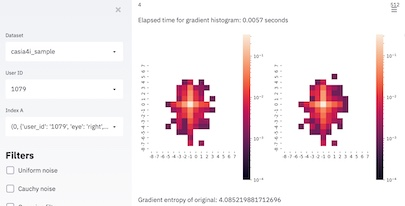
\includegraphics[width=1\linewidth]{figures/labs/EntropyLab}
		\caption{Entropylab}\label{fig:tools:entropylab}
	\end{subfigure}
	\hfill
	\begin{subfigure}{0.3\textwidth}\centering
		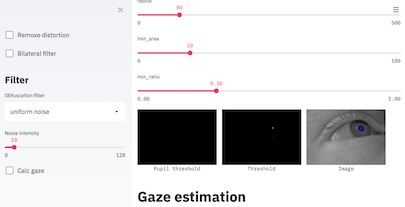
\includegraphics[width=1\linewidth]{figures/labs/GazeLab}
		\caption{GazeLab}\label{fig:tools:gazelab}
	\end{subfigure}
	\hfill
	\begin{subfigure}{0.3\textwidth}\centering
		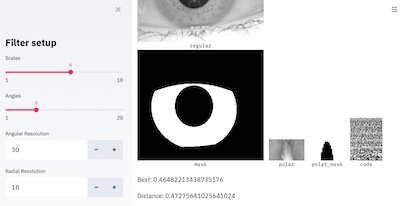
\includegraphics[width=1\linewidth]{figures/labs/ObfuscationLab}
		\caption{ObfuscationLab}\label{fig:tools:obfuscationlab}
	\end{subfigure}
	\\
	\begin{subfigure}{0.3\textwidth}\centering
		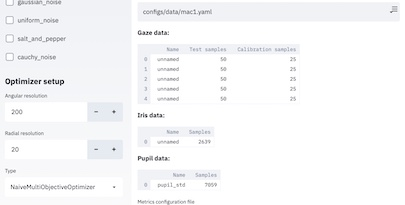
\includegraphics[width=1\linewidth]{figures/labs/OptimisationLab}
		\caption{OptimisationLab}\label{fig:tools:optimisationlab}
	\end{subfigure}
	\hfill
	\begin{subfigure}{0.3\textwidth}\centering
		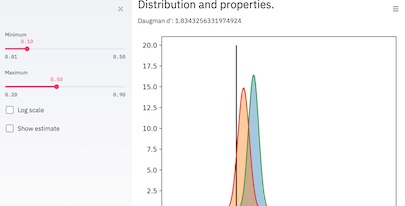
\includegraphics[width=1\linewidth]{figures/labs/ObfuscationResultAnalyser}
		\caption{ObfuscationResultAnalyser}\label{fig:tools:obfuscationresultanalyser}
	\end{subfigure}
	\hfill
	\begin{subfigure}{0.3\textwidth}\centering
		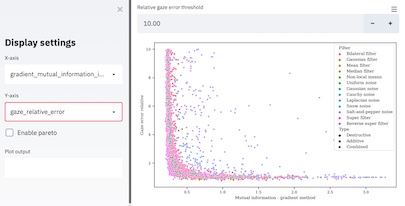
\includegraphics[width=1\linewidth]{figures/labs/OptimisationResultAnalyser}
		\caption{OptimisationResultAnalyser}\label{fig:tools:optimisationresultanalyser}
	\end{subfigure}
	
	\caption{Screenshots showing the individual interactive tools. The code is, of course, included with the thesis submission as well.}\label{fig:tools}
\end{figure}

In terms of the optimisation experiment described in the article, each obfuscation method represents one MultiObjectiveOptimizer instance. To make experimentation and repeatability easier, a number of interactive tools are created using StreamLit which is a Python library for creating data-rich, interactive, web applications.

Six different interactive tools were created - some for experimenting with 
\begin{description}
	\item [EntropyLab] Tool for experimenting with image-based entropy measurements and their distributions.
	\item [GazeLab] Tool for experimenting with gaze estimation parameters and evaluating performance.
	\item [ObfuscationLab] Explorative tool for testing the iris obfuscation algorithm and setting up configuration files for large-scale testing. 
	\item [OptimisationLab] Tool used for running small optimisation experiments and creating configurations for larger ones. 
	\item [ObfuscationResultsAnalyser] For testing the result of running the iris obfuscation experiment. Only allows simple analyses and was mostly used during development of the iris recognition algorithm to test performance.
	\item [OptimisationResultsAnalyser] Detailed interactive analysis for the parameter experiments. It has been used primarily to discover interesting facets of the results. Due to the large number of metrics used for analysis, interactive visualisations provide....
\end{description}


\section{Gaze estimation}
For this project, I chose to implement my own gaze estimation system. Although previous students at ITU have developed eye tracking software which was available to me, both the system and the hardware was not ideal for this use case either. 

The physical setup is a remote camera that is positioned close to the eye to create circumstances similar to head-mounted eye trackers. Participants are asked to rest their head on a stand which ensures relative stability of the eye's location relative to the camera. A screen is used to show target which are to be predicted by the software. An infrared LED fastened to the screen acts as both a light and for creating a corneal reflection. Details on calibration are left to the article.

To estimate the gaze point from any given image, the system uses a pupil-glint vector as a source which is then mapped from image to screen coordinates using a two-dimensional polynomial. The glint effectively acts as an origin for the system since it is stationary. The coefficients of the polynomial are found using the least-squares method on a set of calibration points where the target screen position is known.

For a set of pupil-glint vectors $\{\mathbf{x}^1, \mathbf{x}^2, \dots, \mathbf{x}^n\}$ and corresponding screen positions $\{\mathbf{y}^1, \mathbf{y}^2, \dots, \mathbf{y}^n\}$, a second-degree model requires two functions of both input variables which can be written
\begin{equation}
    \mathbf{y}^i =  \begin{bmatrix}
        \left(x_1^{1}\right)^2 & \left(x_2^{1}\right)^2 & x_1^1x_2^1 x_1^1 & x_2^1 & 1\end{bmatrix} \begin{bmatrix}a^1&a^2\\ b^1&b^2\\ c^1&c^2\\ d^1&d^2\\ e^1&e^2\\ f^1&f^2\end{bmatrix},
\end{equation}
where $a$-$e$ are the parameters. A solution could be found using $12$ calibration points, but the method of least squares allows us to minimise the impact of outliers.

Several pupil detectors were tested, of which DeepEye (REF) outperformed the others. Specifically, I tested a home-made BLOB based detector and the ElSE and ExCuSE detectors as well (REFS), although they all failed on some easy samples as shown (FIGREF). DeepEye is a neural network and .....
% TODO: Skriv også om deepeye i metode...

\subsection{Iris recognition}
The iris recognition implementation is an attempt at closely matching the design of the original algorithm created by Daugman (REF) and which is generally still used for baseline comparisons today. In improved versions, Daugman's method acheives accuracies of XX on a non-public dataset. The replica only achieves XX on the CASIA IV dataset though it should be mentioned that this is very favourable compared to other replicas proposed in various studies (REF). Additionally the test dataset, CASIA IV, only contains $2639$ samples from $xx$ subjects which limits the precision of the result.

The reasons for implementing the method from scratch are twofold. By far the most important was that no accurate implementation was available with support for Python. The OSIRIS project (REF) has seemingly disappeared and several others including (REFS) did not use the original technique. A very thorough implementation of multiple iris recognition algorithms a available in a library (REF) but only in c++. Writing a Python interface was outside the scope of this thesis. Secondly, implementing the method from scratch provides valuable experience which is useful when trying to understand how the iris signal is communicated and decoded from its image representation.


Daugman's method is based on the use of wavelets to detect the phase of the iris at a number of frequencies and angles. The minimum wavelength chosen for the filters was 3 pixels in order to avoid artifacting affecting the outcome.

\begin{figure}
    \begin{subfigure}{0.5\linewidth}
        \centering
        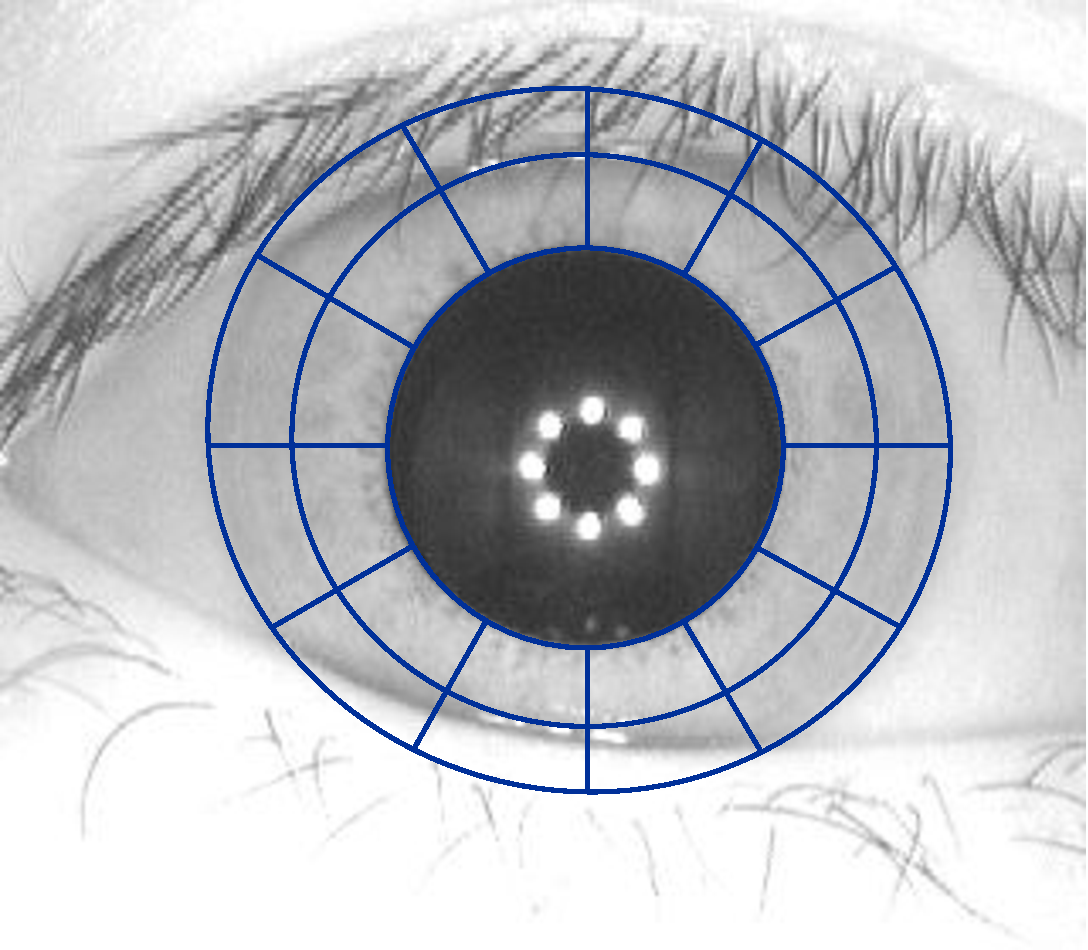
\includegraphics[width=0.6\linewidth]{figures/polar-image.pdf}
        \caption{The pupil and iris circumference ellipses define a polar coordinate system.}
        \label{fig:polar-method}
    \end{subfigure}
    \begin{subfigure}{0.5\linewidth}
        \centering
        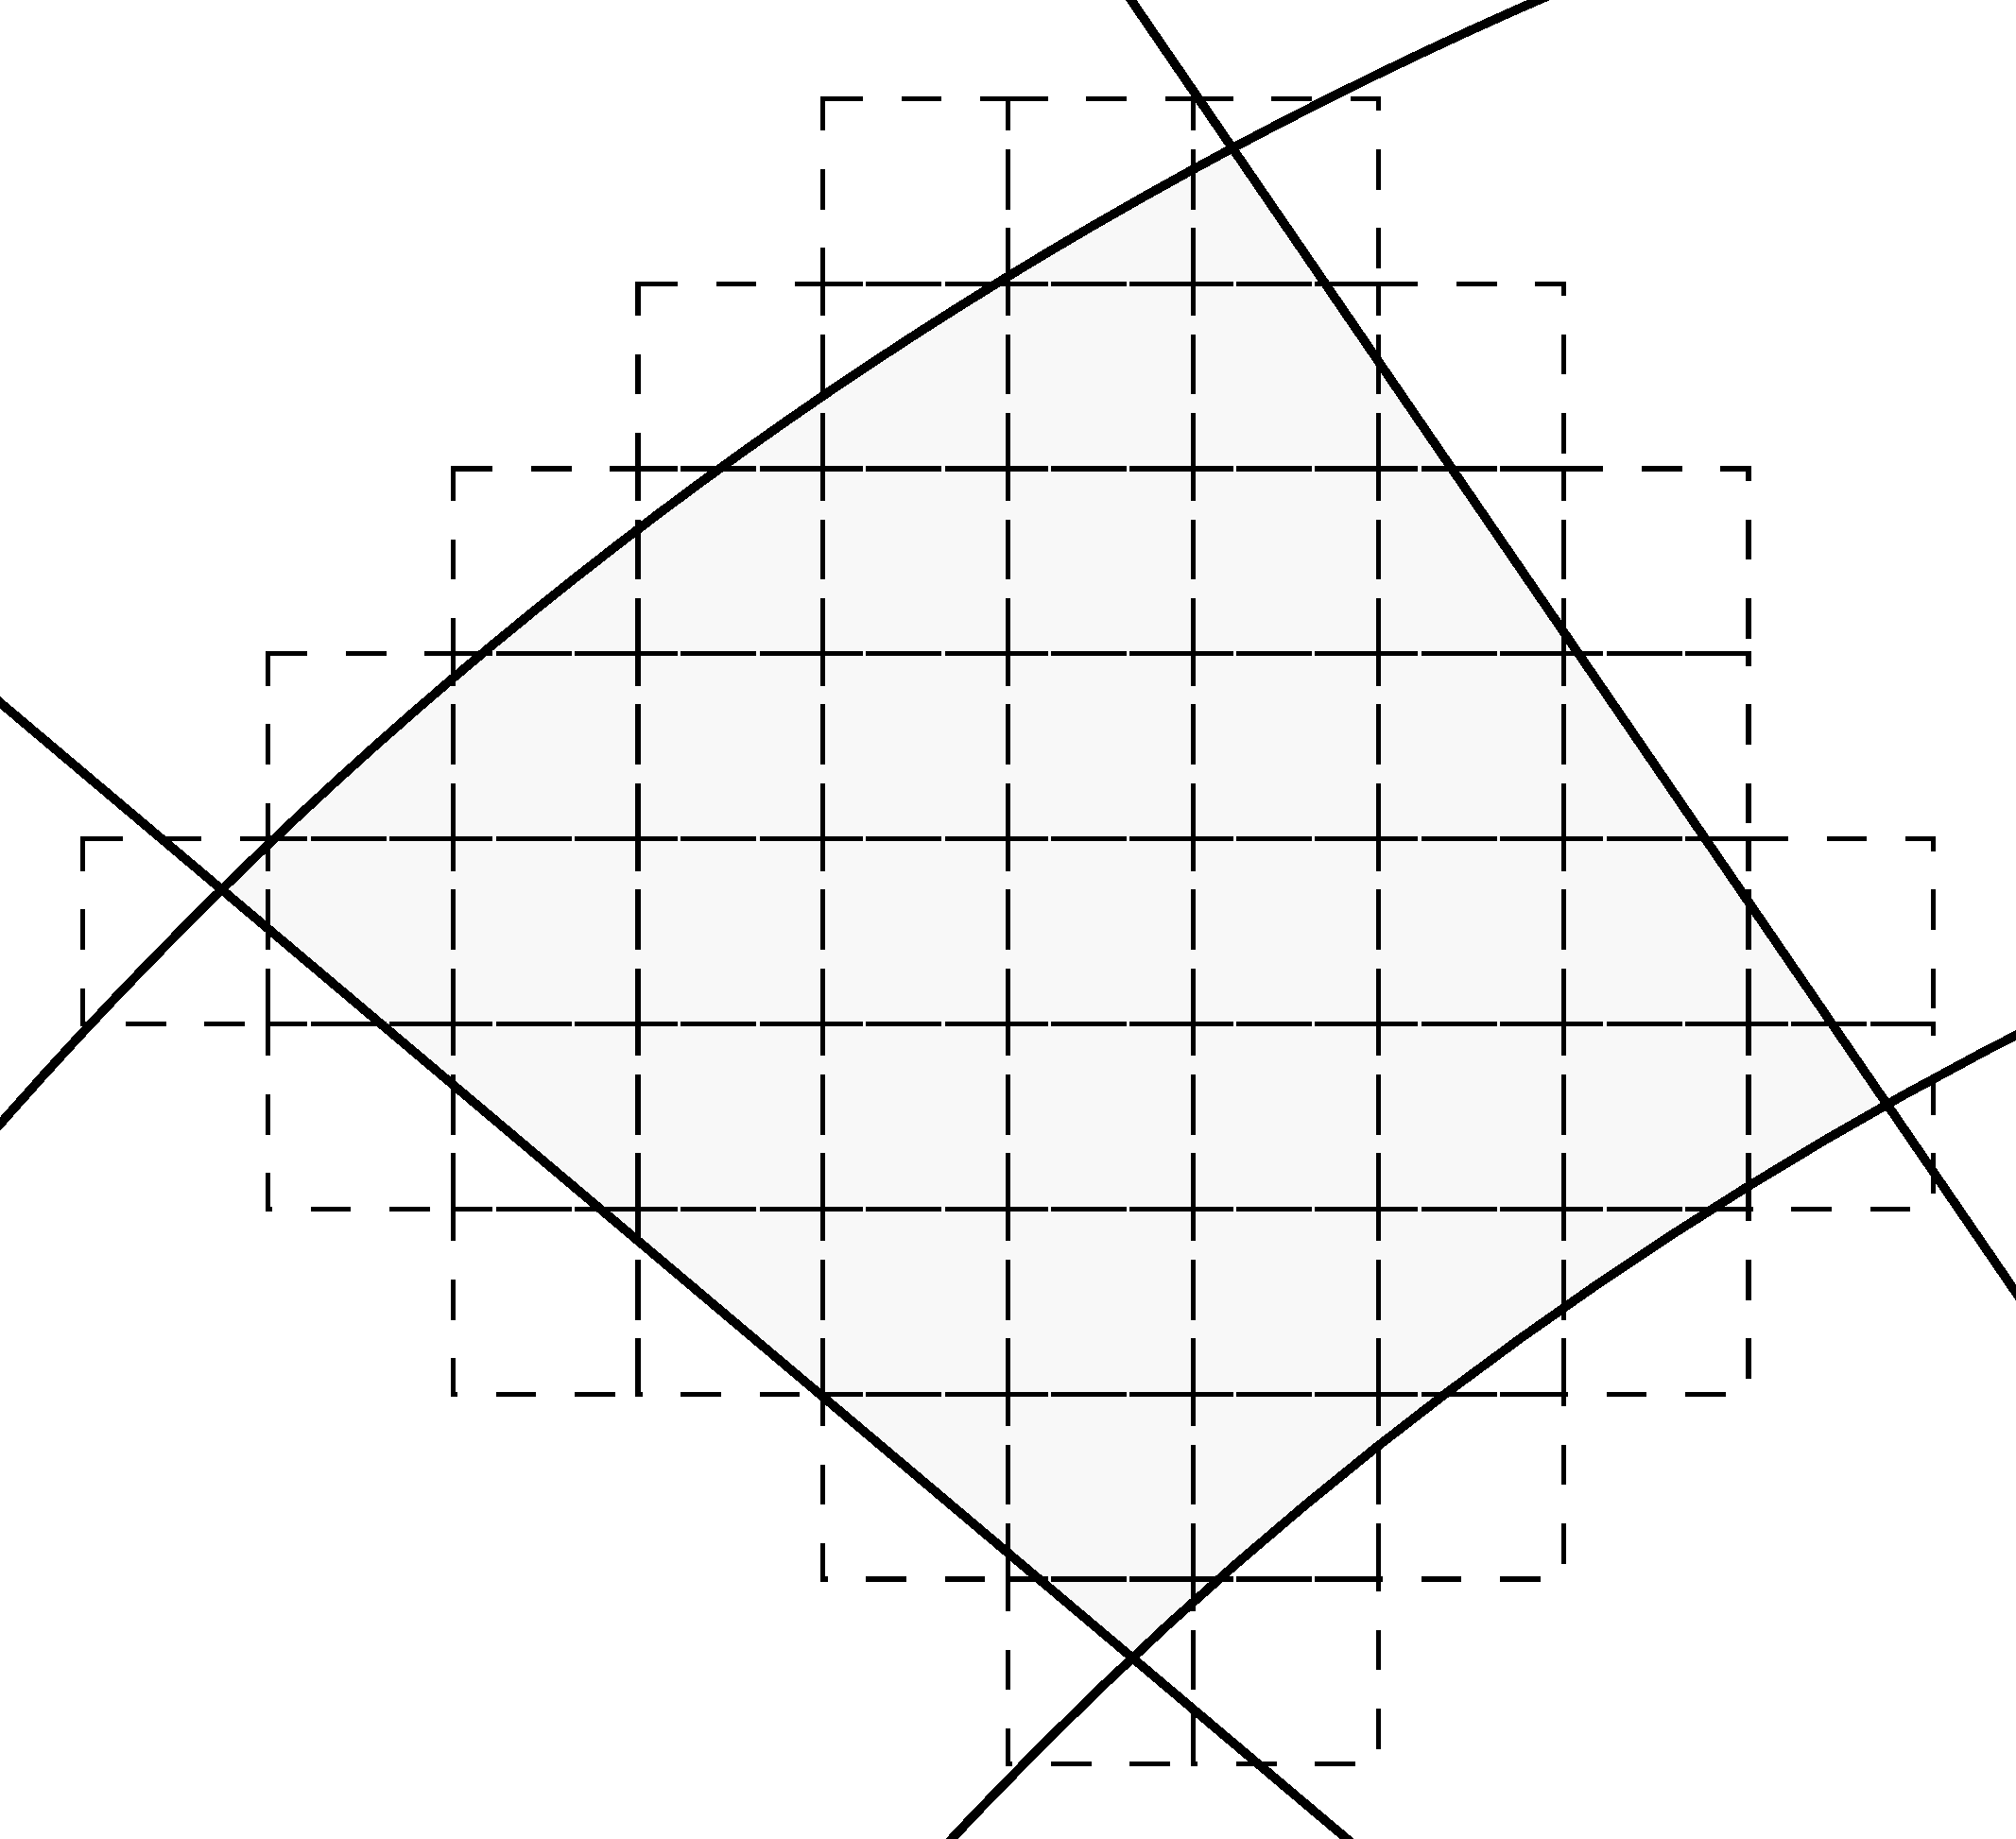
\includegraphics[width=0.6\linewidth]{figures/polar-method.pdf}
        \caption{Individual pixels in the polar coordinate system covers many actual pixels in the original cartesian space. The effect is amplified in the figure.}
        \label{fig:polar-method}
    \end{subfigure}
\end{figure}

The polar sampling method uses a particularly interesting technique. As shown in (FIGREF), the pseudo-polar coordinate system results in pixels that overlap several of the original image's pixels in strange ways. A possible solution would be to radically increase the polar resolution and use billinear sampling or similar for interpolation (REF). 

Due to the relatively slow phase calculation implementation however, I chose to keep the polar resolution low and instead opted to use a simple probabilistic sampling technique. If we denote the polar pixel region as a set $S$, each pixel in the cartesian image coordinate system is similarly sets $C_1, \dots, C_n$. The ideal pixel value at that coordinate is then:
\begin{equation}
    P(S) = \frac{\sum_{i=1}^n I_i A(S\cap C_i)}{A(S)}
\end{equation}

In other words, the pixel should take on the average value of the underlying pixels weighted by their intersecting areas. An easy way to implement this is by randomly sampling points inside $S$, adding their values, and dividing by $n$
\begin{equation}
    P(S) = \frac{1}{n}\sum_{x \sim U(S)}^n I_{x},
\end{equation}
where $U(S)$ is a uniform distribution over $S$. This method works for any size...

\begin{figure}
    \centering
    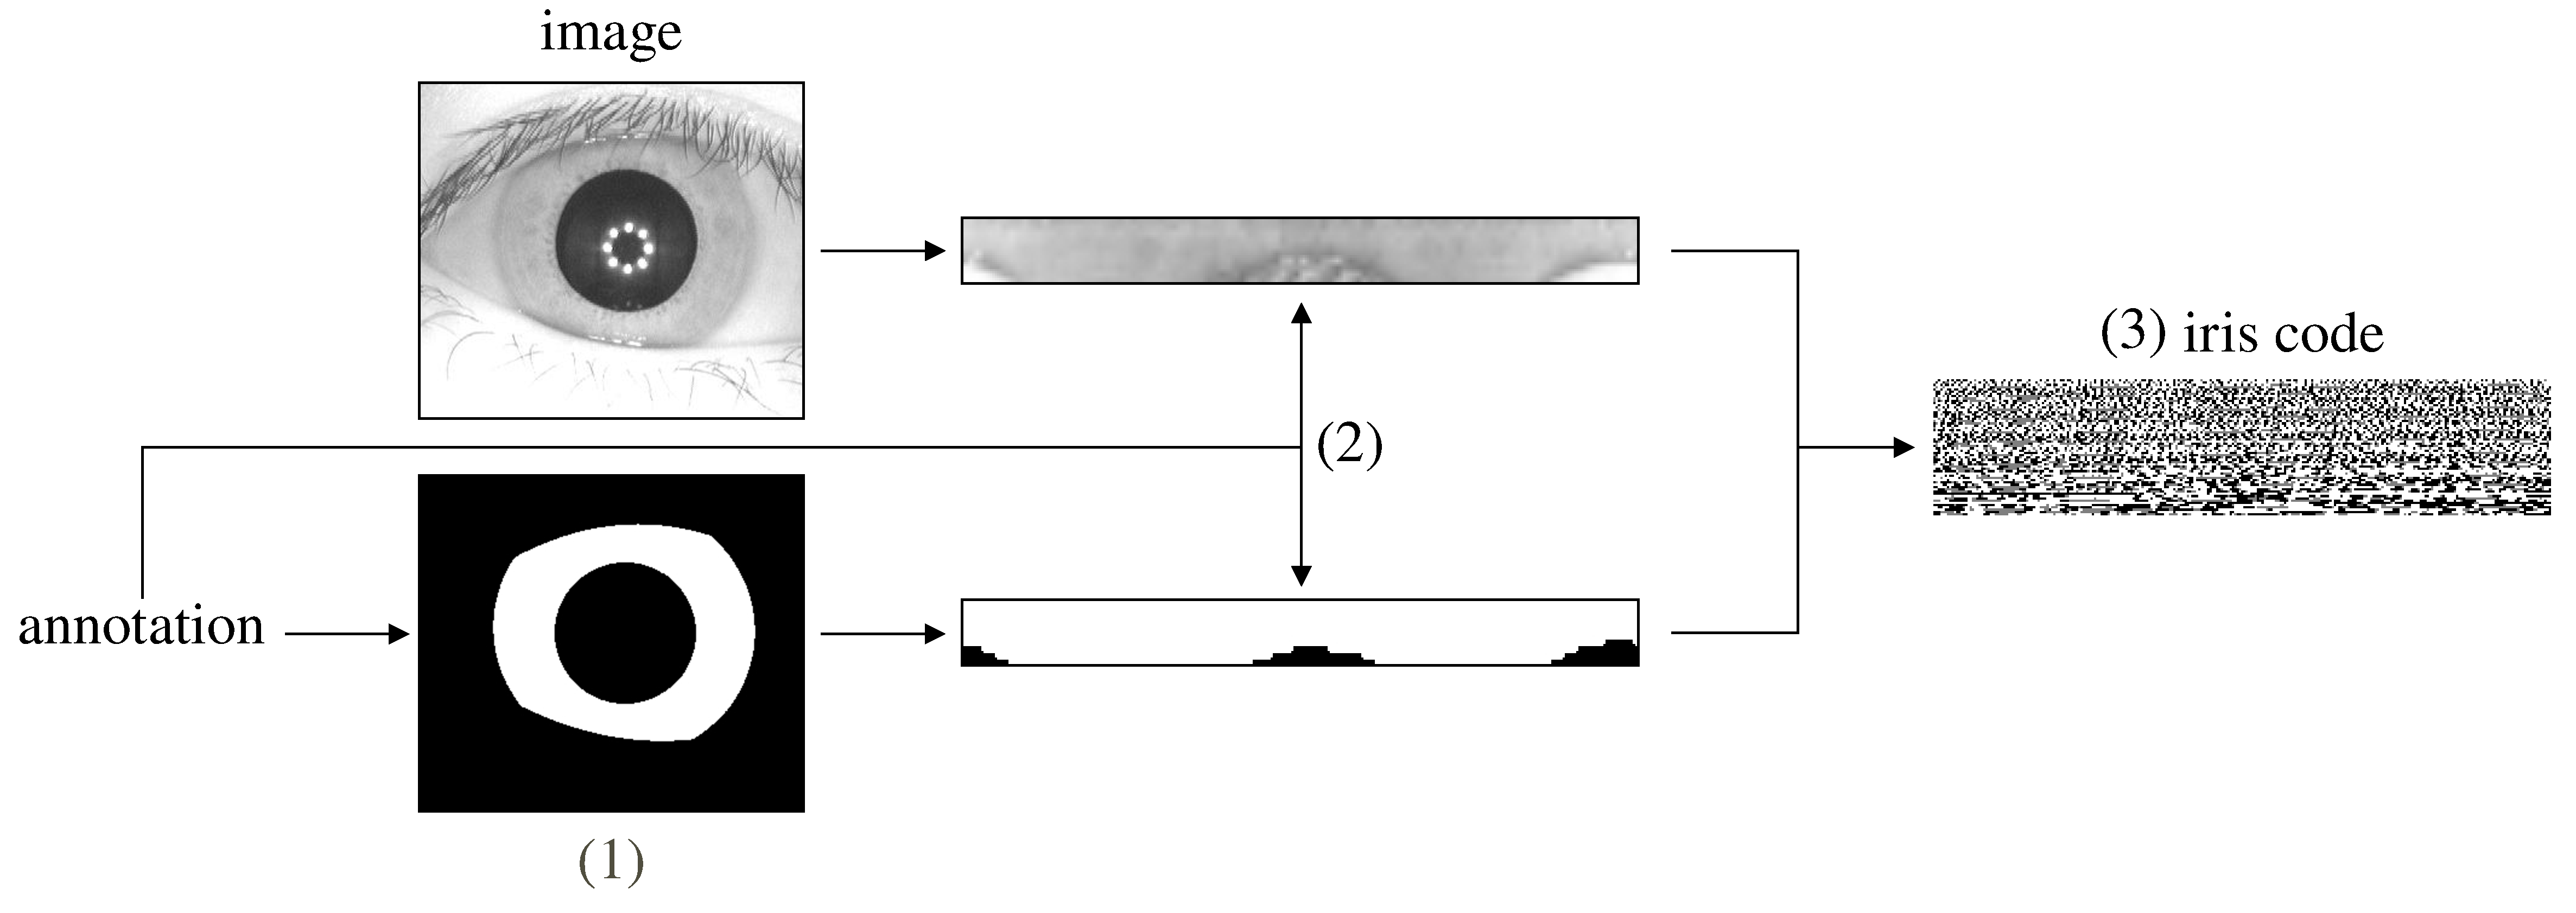
\includegraphics[width=1\linewidth]{figures/iris-code-gen.pdf}
    \caption{Iris code generation process. (1) The annotation (see text) is used to generate a binary mask of the visible parts of the iris. (2) The pupil and iris boundaries are used to create dimensionless polar projections of the iris and mask. (3) Gabor filters are applied to the polar image, quantized, and concatenated to a $16000$-element bit-vector which is the iris code. It is here visualised using black pixels for the value $0$ and white pixels for the value $1$. Pixels masked by the polar mask projection (and excluded from comparisons) are shown in grey (zooming might be necessary). }
    \label{fig:iris-code-gen}
\end{figure}

\section{Optimisation system}
Iris obfuscation has at least two objectives, one for the gaze accuracy and one for the iris recognition accuracy. This is problematic for classical optimisation where the goal is to find an extremum of a cost function with $\mathbb{R}$ as its domain. The field of multi-objective optimisation deals with exactly this kind of situation. A possible solution is to define a weighing of each sub-objective, i.e.
\begin{align}
	J^{\mathcal{O}}(I) = w_{gaze}J_{gaze}^{\mathcal{O}}(I) +  w_{iris}J_{iris}^{\mathcal{O}}(I),
\end{align}
as originally suggested by my supervisor in (REF). This approach may be suitable when sufficient knowledge about the problem makes it possible to define reasonable values for the weights. It does, however, assume prior knowledge of the relative importance of the objectives. 

Instead, this study focuses on exploring the trade-offs between various objectives over a large range of possible parameter values for each obfuscation method. In the article this is done using grid-search due to the relatively limited search space. I also experimented with a population-based method for combining multiple objectives which preserves (something).

A central idea in using these explorative methods is \textit{pareto optimality}. Pareto optimality is based on the concept that even when objectives are not comparable, it is possible to determine an ordering of the optimality of points. Figure (REF) shows an example in two dimensions. The points marked in blue are objectively better than any of the black points. Being objectively better here means that it is at least as good in every dimension and better in at least one. This is called dominance - the full definition is shown in \cref{def:dominance}. Points that are not dominated by any other point is \textit{Pareto optimal} (\Cref{def:p-optimal}). The subset of all such points of a given set is called the \textit{Pareto frontier} (\Cref{def:p-frontier}). In this example, the blue points define the Pareto Frontier.

\begin{definition}[Dominance]\label{def:dominance}
Given points $\mathbf{x}$, $\mathbf{x'}$ and an objective function $f$ with domain $\mathbb{m}$, $\mathbf{x}$ dominates $\mathbf{x'}$ if and only if
\begin{align}
 \forall i \in \{1, \dots, m\} :&\quad f_i(\mathbf{x})\leq f_i(\mathbf{x'}) \\
and \quad \exists i \in \{1, \dots, m\} :&\quad f_i(\mathbf{x}) < f_i(\mathbf{x'}).
\end{align}
In other words $\mathbf{x}$ cannot be worse than $\mathbf{x'}$ for any objective and has to be better on at least one.
\end{definition}

\begin{definition}[Pareto optimal]\label{def:p-optimal}
A point $\mathbf{x}$ in set $S$ is Pareto optimal if
\begin{align}
    \nexists \mathbf{x'} \in S: \quad \mathbf{x'} \text{ dominates } \mathbf{x}.
\end{align}
\end{definition}

\begin{definition}[Pareto frontier]\label{def:p-frontier}
The subset of all Pareto optimal points in a given set.
\end{definition}

Defining a Pareto frontier for a vector-valued objective function compresses the relevant parameter under consideration to a surface. This means that 

\begin{figure}
    \centering
    \begin{tikzpicture}
    
    \draw[thick,->] (0,0) -- (4,0) node[anchor=north west] {x axis};
    \draw[thick,->] (0,0) -- (0,4) node[anchor=south east] {y axis};
    
    \draw [red] plot [smooth cycle] coordinates {(1,1) (1,3) (3,3) (3,1)};
    \end{tikzpicture}
    \caption{Caption}
    \label{fig:my_label}
\end{figure}



\section{Filtering approaches}
We approach the analysis of separating the iris signal and the gaze signal from a pragmatic perspective. An image may be visualised as a height-map to more clearly display the individual pixel values. 

(FIG) shows an eye image and a one-dimensional slice where the light intensity is graphed as a function of the x-position. Clearly, the portion covering the iris shows relatively chaotic changes but low variance compared to the rest of the image. The pupil-iris boundary and glint-pupil boundary which are used in our gaze-estimation method are clearly identifiable since they are represented as huge changes in intensity. These sorts of examples are typically also shown when introducing image edge detection, since it clearly demonstrates the connection between rate of change, i.e. the gradient, and the presence of an edge. 

When analysing the image as a Fourier series, two important factors stand out. Firstly, the iris seems to be dominated by a low-amplitude, very random signal. This indicates a range of small to medium wavelengths and high entropy. The edge regions, which are used by our gaze algorithm, instead look roughly like square waves. A square wave requires an infinite Fourier series to be represented accurately. Because the image is effectively band-limited, it is possible to recreate it with a finite series but it still spans the whole wavelength spectrum.

This signal analysis becomes important when considering methods for obfuscation. Our understanding of how the transformations affect different simpler signals may help us find suitable methods that are more well-suited to the application.

\subsection{Measuring information in images}
The term signal is rather abstract but is typically defined as a function that encodes or contains information of interest. Signals can be defined over temporal inputs, spatial inputs, or both. In the case of eye information processes, signals such as the captured eye images may be analysed individually as purely spatially divided signals or jointly as a time series of frames. The iris pattern in either its abstract or encoded form, is only resolved spatially while the gaze signal is usually analysed as a time-series. 




When viewed as bandlimited discrete signals of two dimensions, images can be analysed structurally through the 

To measure entropy and mutual information in images, it is necessary to formulate a method for defining the image in terms of a probability distribution. Specifically, it is necessary to define a model for the image distribution and estimate it using the image itself as data.

The fundamental model is that each image can be represented by an unknown distribution $P_{img}$ of an unknown number of random variables $X^1, \dots, X^n$. A simple model is the intensity histogram which estimates a discrete distribution of intensity values assuming that each pixel is independent of each other. It can be defined as
\begin{align}
    P(I=i) = \sum_{x\in\mathcal{X}y\in\mathcal{Y}} \delta_{i, I_{x,y}},
\end{align}
where $\delta_{a, b}$ is the Dirac delta function. The downside to this approach is that no correlations between pixels are considered even though they clearly exist. For use in obfuscation measurement, this is problematic since the iris recognition methods use texture and not direct pixel intensities for detection. 

In the most general terms, the distinct features of an iris pattern represents differences in the amplitude and phase of different frequencies. Many iris algorithms of the Daugman type use spatial phase responses to calculate a robust iris code. These traditional methods generally use some form of wavelet transform to separate spatial frequency-responses (REFS). The convolutional neural-network based methods likely learn similar approaches as they have been shown to learn typical bandpass-filters like the wavelets used by Daugman (REF). 

The image derivative, defined by its two partials, has excellent properties for measuring image texture complexity. The image derivative retains all information necessary to reconstruct the original image and is therefore still a valid upper bound on information measures (REF). By defining $P_{img}$ as a joint distribution of the partial derivatives of the image
\begin{align}
    P(dx=i, dy=j) = \sum_{x\in\mathcal{X}y\in\mathcal{Y}} \delta_{i, {I_{\Delta x}}_{x,y}} \delta_{j, {I_{\Delta y}}_{x,y}},
\end{align}

Additionally, we also define joint distributions on convolutions with complex Gabor wavelets. A Gabor wavelet works as a bandpass filter, i.e. it responds only to certain frequency ranges. Defining a joint distribution over the Gabor response of a particular filter makes it possible to measure the entropy in certain frequency ranges which further... By definition however, a bandpass filter does not retain all the information in the original signal and can therefore not be used for definition of upper bounds.




\subsubsection{Filters}

\begin{figure}
    \centering
    \includegraphics[width=1\linewidth]{figures/filter_effect.pdf}
    \caption{Shows effect of applying the proposed filters. The heat-maps show the corresponding gradient histogram.}
    \label{fig:filters}
\end{figure}
Specifically, one of the previous studies tested a Gaussian filter (and optical defocus) (REF) for obfuscation based on the assumption that the lowest frequency wavelength of the pupil edge would be enough to enable robust gaze estimation. The problem with the Gaussian filter is that it is a low-pass filter, i.e. it removes high-frequency components. Since sharp edges are only sharp because of these, a Gaussian filter makes images look blurry and unsharp as a result. The effect on the image in (FIG) is shown in (FIG), where a Gaussian filter with $\sigma=5$ has been applied. Clearly, the gradient at the edge has been smoothed considerably. The reason the study still reports favourable results is that the gaze-estimation algorithm is likely robust to at least some degree of edge blurring.

A smarter approach is to consider not just the spatial neighbourhood but the intensity as well. 
\section{Experiments}
This work focuses on a detailed analysis of the effect the proposed obfuscation methods have on the concurrent goals of iris obfuscation and gaze estimation over a wide range of parameter values. Because iris recognition performance is computationally expensive, the analysis is divided into two separate experiments, one for providing detailed information on the effect of obfuscation for a large number of parameter configurations, and one for providing complete ...



The proposed methods have been extensively evaluated on a number of relevant metrics and datasets (which ones?)...... The results provide a clear image of the effectiveness of the individual methods and provide us with enough detail to help us understand how they affect gaze estimation and iris recognition.

Two experiments have been performed, (1) a systematic search of filter parameters and their influence on utility, security, mutual information, and other metrics, and (2) test of iris recognition performance on the full dataset + maybe some additional gaze tests?


For the experiments we used different datasources for gaze estimation and iris recognition in order to provide favourable conditions for iris recognition. The dataset used for iris recognition, CASIA IV, is generally considered easy for iris recognition, which is good in this case since it is exactly the opposite when the goal is to prevent correct recognition.


\subsection{Eye tracker setup}



The gaze dataset was recorded using a remote camera placed close to the eye to simulate the location on head-mounted eye trackers. A chin rest was used for keeping the head stable during recording. The participants were asked to fixate on a number of targets on a screen placed approximately 60cm from their head. A single infrared LED provides a glint used for normalisation. A set of 25 calibration images and 50 test images were recorded for each participant, with the calibration samples being placed in a regular grid and the test images being sampled from random uniform distributions.



\paragraph{Gaze estimation}

The gaze model used is a 2nd degree polynomial using a pupil-glint vector as its normalised input. The method requires detection of the pupil which is done by the DeepEye network (REF) and detection of the glint which is done using image thresholding and BLOB detection. 

\subsection{Iris recognition}

For iris recognition, we made an iris recognition algorithm that models Daugman's method as closely as possible, i.e. it uses a quantisation of phase over the iris region as the identifying code. The \emph{hamming distance} between codes is used to model distributions for matches and non-matches respectively, which are finally used to select a threshold used to determine, whether a comparison should be accepted or discarded. As in Daugman's articles, the complex 2d Gabor function is used as a bandpass filter. Phase quantisation is applied to the result to produce two bits of iris code for each Gabor application location. We ended up using 4 scales and 6 angles per scale. Since gabor filters do not have an orthogonal basis, these filter banks are selected empirically. 

Base iris recognition performance is shown in (FIGREF) and is acceptable compared to other similar algorithms. 
Without obfuscation, the algorithm performs favourably compared to many other iris recognition algorithms (refs) and is within a few orders of magnitude of the original. Larger datasets and a direct comparison would be needed to accurately determine the real-world performance. 

However, the process of determining iris recognition performance on a given dataset requires many samples to produce reliable results. Specifically, given $n$ comparisons of different source irises and $m$ comparisons of equal irises, the false acceptance rate can only be determined in increments of $1/n$ and the false rejection in increments of $1/m$. Assuming the distributions approximate normal distributions (Daugman REF), their means and variance estimators have variance $Var(\bar{X})=\sigma^2/n$ and $Var(S_n)=\sigma^4/(n-1)$ respectively .... and so on...

We therefore choose to only perform actual iris recognition for a few select parameters for each filter. The iris recognition comparison uses the CASIA IV dataset (REF). A subset of $2,600$ images which have been manually segmented are used (REF). This removes any influence an iris detection mechanism might have and thus provides optimal conditions for effective iris recognition. Additionally, the dataset itself is relatively easy, which purposefully makes obfuscation as difficult as possible and thus should increase our trust in the results.





\subsection{Parameter experiment}
A grid-search was performed for each obfuscation method with linearly spaced parameter values. For each parameter configuration a selected number of metrics were evaluated on samples drawn from the respective iris, gaze, and pupil-centre datasets using the obfuscation and transformed using the relevant obfuscation method. Searching the parameter space in this systematic manner has the advantage of presenting us with a more complete picture of how the various metrics react to parameter changes over the whole spectrum of possible values. Parameter configurations and precise metric descriptions are found in appendix??. 

Importantly, the random sampling makes the results stochastic as well, which is why these results are not used for evaluation directly. This necessary trade-off allows a significant increase in the number of parameter values tested which provides insight into how the different methods work and compare.

\subsection{Evaluation experiment}
The evaluation experiment tests iris recognition performance on the complete set of $2,600$ iris images. This results in $xx$ possible code comparisons for each test. Two testing methodologies are used for evaluating the obfuscation methods. For both, the iris codes for the entire dataset are computed for a selected number of parameter configurations for each obfuscation method.

The first test compares the iris codes from the obfuscated images with the original iris codes derived from the unmodified images. The resulting distances thus reflect data from a situation where the obfuscated data is checked against an existing iris database for matches. 

The other test compares the obfuscated codes internally and therefore reflect the possibility of constructing a new iris database from obfuscated images and using it for subsequent identification. 

Both tests are equally relevant. The former determines whether the obfuscation methods can be used as safeguards against being recognised using a known reference while the latter determines if obfuscated images can related ..... Both situations are problematic as...

\chapter{Discussion}
This chapter is an extension to the article with additional analysis of the results and a more thorough discussion of how the results support the proposed model and what insights the results give to support its use for other applications.

\section{A detailed look at obfuscation method information}
\begin{figure}
	\centering
	
	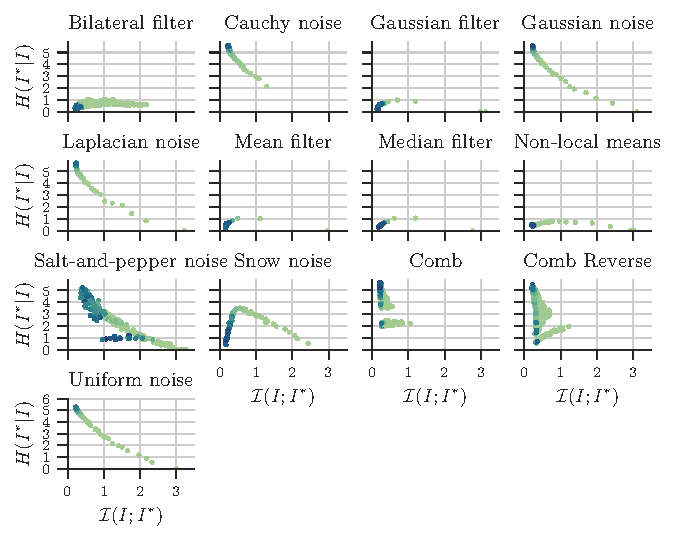
\includegraphics[width=1\textwidth]{figures/results/individual}
	
	\caption{Plot of mutual information and conditional information response for individual filters. Note that these distributions are estimated from the entire image, producing less noisy results than the ones presented in the article.}\label{fig:individual}
\end{figure}

\Cref{fig:individual} shows mutual information and conditional entropy for each filter separately. This makes the distinction between them even more noticeable. 

The noise methods, except snow and salt-and-pepper, all follow an almost straight line, "converting" mutual information into conditional entropy. \Cref{fig:individual-entropy} is similar, but with the output image entropy as its x-axis. From this figure it is clear that for all noise methods, the increase in conditional information is roughly proportional to the increase in entropy, but not at a one-to-one scale. As shown in \cref{eq:entropy-law}, this necessitates a loss in mutual information, i.e. $\mathcal{I}(I^*;I) = H(I^*) - H(I^*|I)$. Since the entropy and conditional entropy are roughly linearly correlated for the noise-based methods, we have $H(I^*) \approx \alpha H(I^*|I) + H(I)$ and as a consequence, the mutual information can be expressed as a function of the conditional entropy and the entropy of the original image 
\begin{align*}
\mathcal{I}(I^*;I) \approx (\alpha-1)H(I^*|I) + H(I).
\end{align*}
This is of course only an approximation.

The snow method has a sudden drop in conditional information which is caused by its definition. At low densities, snow increases conditional entropy because the randomly placed pixels adds high gradient components. At higher densities however, the fact that only the value $127$ is used for pixels starts to decrease the entropy significantly. %The uniform snow method is susceptible to the same effect when gaussian variance is low and \todo{what about this?}

\begin{figure}
	\centering
	
	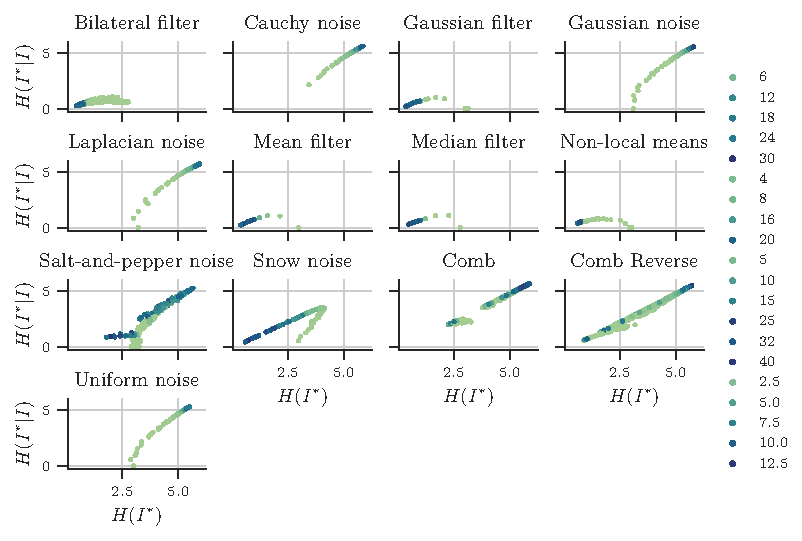
\includegraphics[width=1\textwidth]{figures/results/individual-ent}
	
	\caption{Plot of entropy of the obfuscated images and conditional information response for individual filters.}\label{fig:individual-entropy}
\end{figure}

The filter-based methods behave as explained in the article and mainly impact mutual information. The combination methods, and especially Comb, is worth investigating further. \Cref{fig:comb} uses the same axes as \cref{fig:individual} but displays only data from the Comb method and with the colours indicating the three parameters in the respective plots. The scale parameter, $\gamma$, correlates directly with the value of conditional entropy as expected. The generally lower mutual information values are likely caused by a narrower band of parameters used for the experiment due to time considerations. It shows that the diagonal bands visible in the figures corresponds to the response caused by the bilateral filter. It correlates highly with the color variance parameter $\sigma_c$ but is seemingly independent from the spatial parameter $\sigma_s$. This effectively means that only small values of $\sigma_s$ is needed.

\begin{figure}
	\centering
	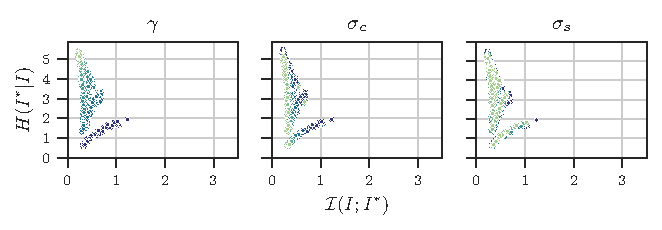
\includegraphics[width=1\textwidth]{figures/results/comb}
	\caption{}\label{fig:comb}
\end{figure}
\todo{Discuss camera effects}

\subsection{Filters and gradient entropy}
Although the approach to filtering has been argued extensively in the article, it did not show how visually appropriate the gradient entropy is compared to a simple intensity entropy. \Cref{fig:delentropy} shows a number of sample images for which both the intensity histogram and gradient histograms have been calculated. It is visually very clear how the gradient histogram and its entropy corresponds with the visually perceived image complexity.

\begin{figure}
    \centering
    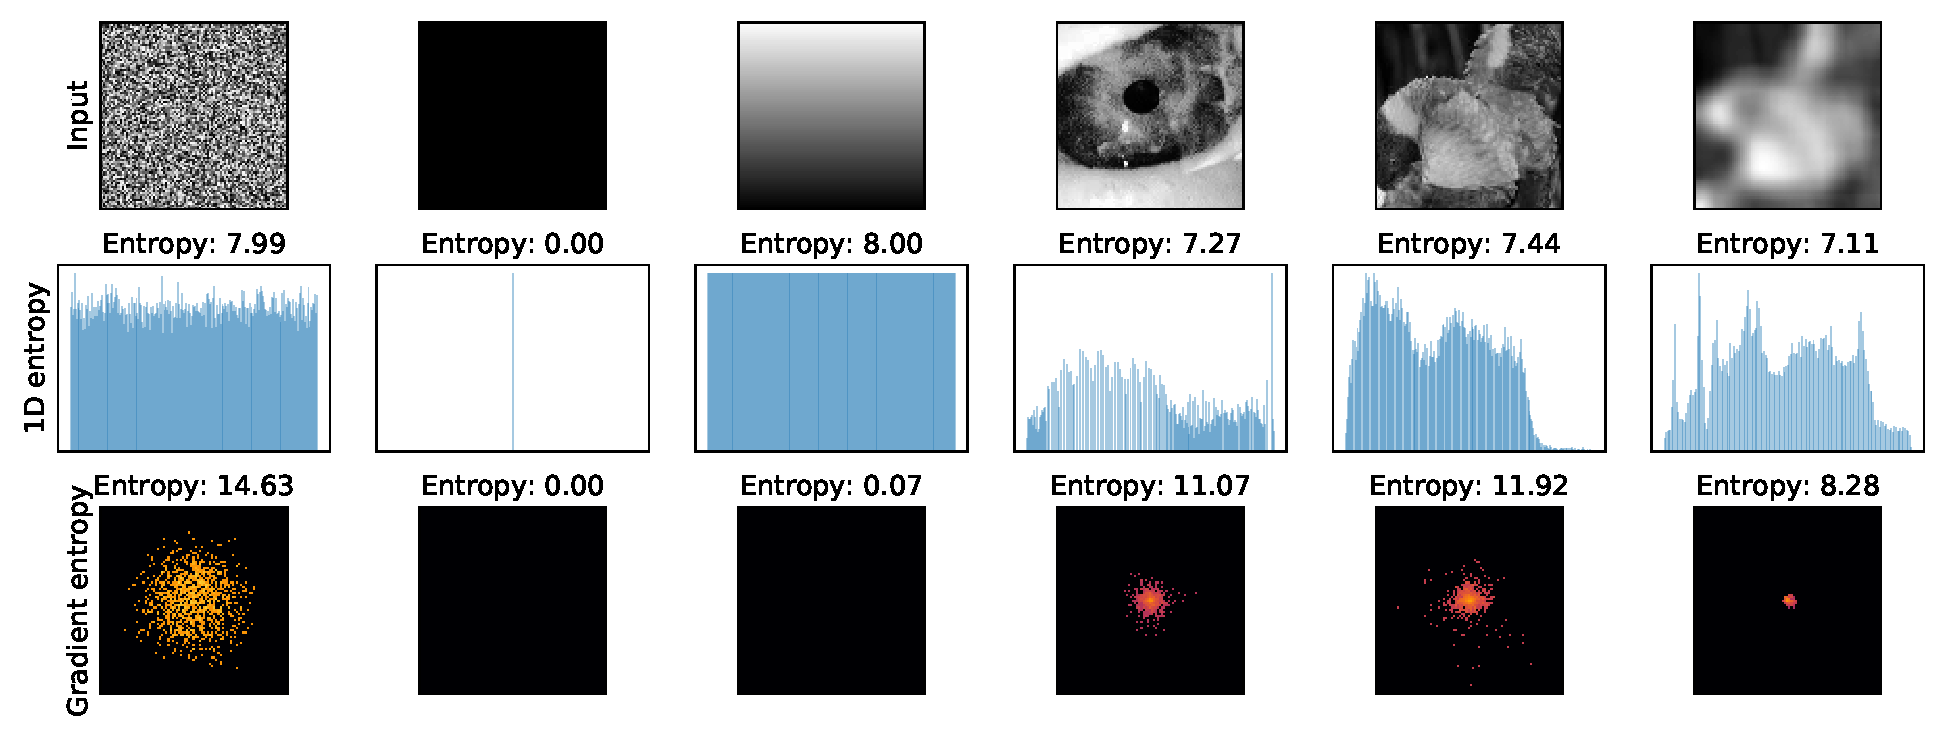
\includegraphics[width=1\linewidth]{figures/results/delentropy}
    \caption{Comparison between entropy of intensity and gradient histograms for a number of image samples.}
    \label{fig:delentropy}
\end{figure}

Sample applications of the proposed obfuscation methods are shown in \cref{fig:filters} where the same visual correlation is still clearly present. The Comb method is also visually indicative of its effectiveness as an obfuscation method because of the clear blurring of eye details while retaining a layer of noise. The parameters used in this example are exaggerated to increase the perceivability of the effects.

\begin{figure}
    \centering
    \includegraphics[width=0.85\linewidth]{figures/results/filter_effect.pdf}
    \caption{Shows effect of applying the proposed filters. The heat-maps show the corresponding gradient histogram.}
    \label{fig:filters}
\end{figure}


%Specifically, one of the previous studies tested a Gaussian filter (and optical defocus) \parencite{BRENDAN_BLUR} for obfuscation based on the assumption that the lowest frequency wavelength of the pupil edge would be enough to enable robust gaze estimation. The problem with the Gaussian filter is that it is a low-pass filter, i.e. it removes high-frequency components. Since sharp edges are only sharp because of these, a Gaussian filter makes images look blurry and unsharp as a result. The effect on the image in (FIG) is shown in (FIG)\todo{do it}, where a Gaussian filter with $\sigma=5$ has been applied. Clearly, the gradient at the edge has been smoothed considerably. The reason the study still reports favourable results is that the gaze-estimation algorithm is likely robust to at least some degree of edge blurring.

%A smarter approach is to consider not just the spatial neighbourhood but the intensity as well. 

\section{Eye information process model generalisation}\todo{ikke klart hvem der siger det...}
For the model and methodology presented in this thesis to be useful, it has to be relevant to the way this category of problems are perceived and to how they are evaluated. For the specific application of iris obfuscation, this has been argued extensively in the article. At an abstract level, the model is used to understand the problem of iris obfuscation and for proposing reasonable and interesting solution candidates. At a concrete level, the information-based metrics and methods derived for calculating them for images showed a high correlation with the observed iris recognition accuracy.

The definition of the model itself as a Bayesian network or as a communication system is an expression of the similarity of image and signal manipulation operations and, by extension, of obfuscation methods in general. The optimisation goal defined for iris obfuscation is thus the same for any other obfuscation problem. The gaze signal itself contains information that has been shown to reveal multiple properties of the recorded subject and is therefore an obvious candidate for using the model. The model and methodology presented here can be applied directly. 

If applied to other problems, results become easier to analyse and compare, and the methodology itself will develop which might provide additional insight into already published material. 

\section{Differential privacy}
Differential privacy is too strict to be a realistic measure for proving privacy bounds for obfuscation tasks. Specifically, only low privacy-bounds are achievable by the application methods proposed so far in the literature. I here present the argument that this is caused by the properties of differential privacy when applied in this domain. Differential privacy is simply a measure of how much a random function impacts the predictability of changing a single element in a set of data points, e.g. an image. Formally, a random function $\mathcal{K}$ is $\epsilon$-differentially private if
\begin{align}
	P[\mathcal{K}(D_1)\in S] \leq \exp{\epsilon} P[\mathcal{K}(D_2)\in S],
\end{align}
for all subsets $S$ of the image of $\mathcal{K}$ and all datasets $D_1$, $D_2$ that differ in at most one element \parencite{dwork2006differential}. In other words, a differentially private function decreases the output's dependence on individual data points since this dependence can be used to infer the original data points.

Differential privacy measures for images have been proposed by \parencite{fan2018image}. Importantly, their extension from single pixel changes to neighbourhoods come with a proportional increase in $\epsilon$ for the same amount of randomness, i.e. for a neighbourhood of $n$ pixels, the privacy should be $\epsilon/n$ to achieve the same level of protection as when a single element is changed. The solution presented in this study suggests an aggressive downsampling using averaging to achieve reasonable levels of noise. Specifically, for an image with pixel intensities in the range $0-255$, and using laplacian noise, the scale parameter is $\frac{255n}{b^2}$ where $b$ is the side length of grid cells defining regions to be averaged. Since laplacian noise has a variance of $2s^2$ where $s$ is the scale, even a low-resolution image of $100\times 10$ pixels (the size used for polar iris images in this work) would require laplacian noise with a variance of $\approx 130\times 10^9$ thus rendering the image practically unusable.

The method proposed in \parencite{BRENDAN_SNOW} does, however, use a weaker form of differential privacy allowing an extra constant term $\delta$ which signifies a probability of leaking information. They prove that $\delta$ has a maximum of $0.5$ for the snow method which means that each pixel has $50\%$ chance of a leak. However, as presented in \cref{sec:methods}, the method can easily be defeated if multiple samples are available. Additionally, even with a single sample, the method shows only moderate effectiveness at preventing recognition with high precision at low recall values. 

In conclusion, differential privacy is not suitable for determining the security of obfuscation methods due to their high sensitivity and the large areas of pixels that need to be secured. As a final note, this criticism does not concern the aggregation based attempts at differential privacy in eye-tracking mentioned in the article. %Instead it is 
 differential privacy has been shown to be highly effective in other eye-tracking privacy tasks where aggregation is involved \parencite{differential-general, differential-general-two}.

\todo{Try to add the rest here}
% Instead, definitions should be derived from a

%\begin{definition}[Privacy]
%Let $S$ be an eye information signal and $\bar{S} \subseteq S$ a subset describing the sensitive data. 

%Let $\mathcal{A}$ be an arbitrary function for inferring 
%Given an arbitrary information extraction function $\mathcal{A}$, an obfuscation function $\mathcal{O}$, and a signal $S$, the privacy strength of $\mathcal{O}$ is defined as
%\begin{align}
%	P[\mathcal{A}(\mathcal{O}(S)) \cup \bar{S} \neq \empty] \leq \rho,
%\end{align}
%for an arbitrary threshold $\rho$ and for any $\mathcal{A}$.
%\end{definition}
























\section{Discussion}


\chapter{Method}
This chapter presents additional details on the experimental work performed as part of this thesis. It builds directly on the material presented in the article, which describes only the most relevant and critical details. Additional results and experiments are presented in the next chapter.

The primary contribution of this work in terms of implemented software, is the platform designed and created for the experimental work presented in the article. The platform consists of tools for optimisation, entropy calculations, iris recognition, gaze estimation as well as a platform for defining, running, and analysing iris obfuscation experiments. 


\section{Implementation details}
This section presents the scope and important details of the software systems implemented to achieve the goals...

FIGREF shows a high-level diagram of the provided software. 

T


\subsection{Optimisation engine}
In order to support different approaches to optimisation, the component has been designed such that any form of optimisation may be implemented. 

The MultiObjectiveOptimizer class expects an Objective and produces a set of results by calling its run method. The run method is implemented differently for each subclass to support different types of optimisation. The NaiveMultiObjectiveOptimizer does not use feedback for determining parameters for the next iteration and instead relies on sampling based parameter selection - this is the class used in the experiments. Additionally, a PopulationMultiObjectiveOptimizer is an implementation of the so called \textit{vector evaluated genetic algorithm}, which uses population strategies to combine and select parameters. The method is discussed in further detail in SECREF, where its possible uses for future work is considered.

Each optimiser has exactly one Objective. The abstract Objective class only has a single sub-class ObfuscationObjective for now but additional ones would be necessary for other optimisation methods or other optimisation tasks. The purpose of the Objective class is to calculate a set of Metrics given a set of parameters. In ObfuscationObjective this is done as described in the article by using different datasets for different metrics. 

Specifically, the objective object is initialised with a pool of datasets divided into three categories: Iris datasets, Gaze datasets, and pupil centre datasets. As seen on the class diagram, this terminology arises from the fact that the gaze datasets are subdivided. The objective can be initialised with any number of different metrics provided as objects. Calling the \emph{eval} function results in the metrics being calculated for a number of samples drawn from the datasets. The sample size is determined at the moment of initialisation.

Results are recorded in a special Logger object, which wraps a dictionary and provides convenient methods for accessing the data.

\subsection{Interactive tools}
\begin{figure}
	\begin{subfigure}{0.3\textwidth}\centering
		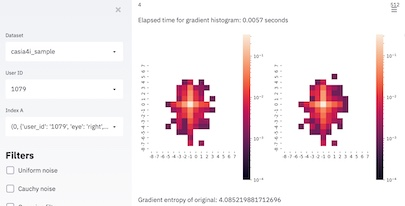
\includegraphics[width=1\linewidth]{figures/labs/EntropyLab}
		\caption{Entropylab}\label{fig:tools:entropylab}
	\end{subfigure}
	\hfill
	\begin{subfigure}{0.3\textwidth}\centering
		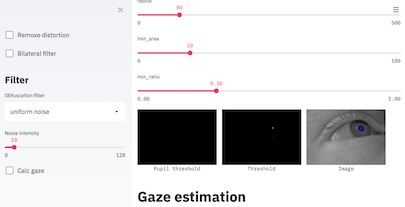
\includegraphics[width=1\linewidth]{figures/labs/GazeLab}
		\caption{GazeLab}\label{fig:tools:gazelab}
	\end{subfigure}
	\hfill
	\begin{subfigure}{0.3\textwidth}\centering
		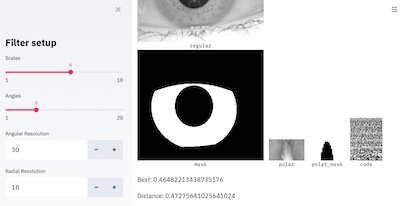
\includegraphics[width=1\linewidth]{figures/labs/ObfuscationLab}
		\caption{ObfuscationLab}\label{fig:tools:obfuscationlab}
	\end{subfigure}
	\\
	\begin{subfigure}{0.3\textwidth}\centering
		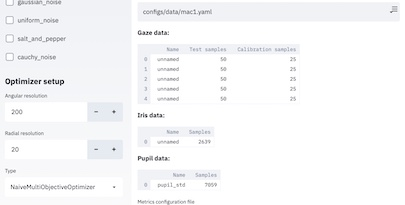
\includegraphics[width=1\linewidth]{figures/labs/OptimisationLab}
		\caption{OptimisationLab}\label{fig:tools:optimisationlab}
	\end{subfigure}
	\hfill
	\begin{subfigure}{0.3\textwidth}\centering
		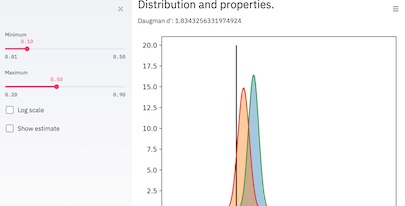
\includegraphics[width=1\linewidth]{figures/labs/ObfuscationResultAnalyser}
		\caption{ObfuscationResultAnalyser}\label{fig:tools:obfuscationresultanalyser}
	\end{subfigure}
	\hfill
	\begin{subfigure}{0.3\textwidth}\centering
		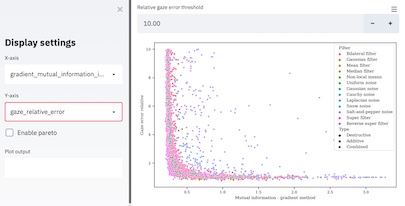
\includegraphics[width=1\linewidth]{figures/labs/OptimisationResultAnalyser}
		\caption{OptimisationResultAnalyser}\label{fig:tools:optimisationresultanalyser}
	\end{subfigure}
	
	\caption{Screenshots showing the individual interactive tools. The code is, of course, included with the thesis submission as well.}\label{fig:tools}
\end{figure}

In terms of the optimisation experiment described in the article, each obfuscation method represents one MultiObjectiveOptimizer instance. To make experimentation and repeatability easier, a number of interactive tools are created using StreamLit which is a Python library for creating data-rich, interactive, web applications.

Six different interactive tools were created - some for experimenting with 
\begin{description}
	\item [EntropyLab] Tool for experimenting with image-based entropy measurements and their distributions.
	\item [GazeLab] Tool for experimenting with gaze estimation parameters and evaluating performance.
	\item [ObfuscationLab] Explorative tool for testing the iris obfuscation algorithm and setting up configuration files for large-scale testing. 
	\item [OptimisationLab] Tool used for running small optimisation experiments and creating configurations for larger ones. 
	\item [ObfuscationResultsAnalyser] For testing the result of running the iris obfuscation experiment. Only allows simple analyses and was mostly used during development of the iris recognition algorithm to test performance.
	\item [OptimisationResultsAnalyser] Detailed interactive analysis for the parameter experiments. It has been used primarily to discover interesting facets of the results. Due to the large number of metrics used for analysis, interactive visualisations provide....
\end{description}


\section{Gaze estimation}
For this project, I chose to implement my own gaze estimation system. Although previous students at ITU have developed eye tracking software which was available to me, both the system and the hardware was not ideal for this use case either. 

The physical setup is a remote camera that is positioned close to the eye to create circumstances similar to head-mounted eye trackers. Participants are asked to rest their head on a stand which ensures relative stability of the eye's location relative to the camera. A screen is used to show target which are to be predicted by the software. An infrared LED fastened to the screen acts as both a light and for creating a corneal reflection. Details on calibration are left to the article.

To estimate the gaze point from any given image, the system uses a pupil-glint vector as a source which is then mapped from image to screen coordinates using a two-dimensional polynomial. The glint effectively acts as an origin for the system since it is stationary. The coefficients of the polynomial are found using the least-squares method on a set of calibration points where the target screen position is known.

For a set of pupil-glint vectors $\{\mathbf{x}^1, \mathbf{x}^2, \dots, \mathbf{x}^n\}$ and corresponding screen positions $\{\mathbf{y}^1, \mathbf{y}^2, \dots, \mathbf{y}^n\}$, a second-degree model requires two functions of both input variables which can be written
\begin{equation}
    \mathbf{y}^i =  \begin{bmatrix}
        \left(x_1^{1}\right)^2 & \left(x_2^{1}\right)^2 & x_1^1x_2^1 x_1^1 & x_2^1 & 1\end{bmatrix} \begin{bmatrix}a^1&a^2\\ b^1&b^2\\ c^1&c^2\\ d^1&d^2\\ e^1&e^2\\ f^1&f^2\end{bmatrix},
\end{equation}
where $a$-$e$ are the parameters. A solution could be found using $12$ calibration points, but the method of least squares allows us to minimise the impact of outliers.

Several pupil detectors were tested, of which DeepEye (REF) outperformed the others. Specifically, I tested a home-made BLOB based detector and the ElSE and ExCuSE detectors as well (REFS), although they all failed on some easy samples as shown (FIGREF). DeepEye is a neural network and .....
% TODO: Skriv også om deepeye i metode...

\subsection{Iris recognition}
The iris recognition implementation is an attempt at closely matching the design of the original algorithm created by Daugman (REF) and which is generally still used for baseline comparisons today. In improved versions, Daugman's method acheives accuracies of XX on a non-public dataset. The replica only achieves XX on the CASIA IV dataset though it should be mentioned that this is very favourable compared to other replicas proposed in various studies (REF). Additionally the test dataset, CASIA IV, only contains $2639$ samples from $xx$ subjects which limits the precision of the result.

The reasons for implementing the method from scratch are twofold. By far the most important was that no accurate implementation was available with support for Python. The OSIRIS project (REF) has seemingly disappeared and several others including (REFS) did not use the original technique. A very thorough implementation of multiple iris recognition algorithms a available in a library (REF) but only in c++. Writing a Python interface was outside the scope of this thesis. Secondly, implementing the method from scratch provides valuable experience which is useful when trying to understand how the iris signal is communicated and decoded from its image representation.


Daugman's method is based on the use of wavelets to detect the phase of the iris at a number of frequencies and angles. The minimum wavelength chosen for the filters was 3 pixels in order to avoid artifacting affecting the outcome.

\begin{figure}
    \begin{subfigure}{0.5\linewidth}
        \centering
        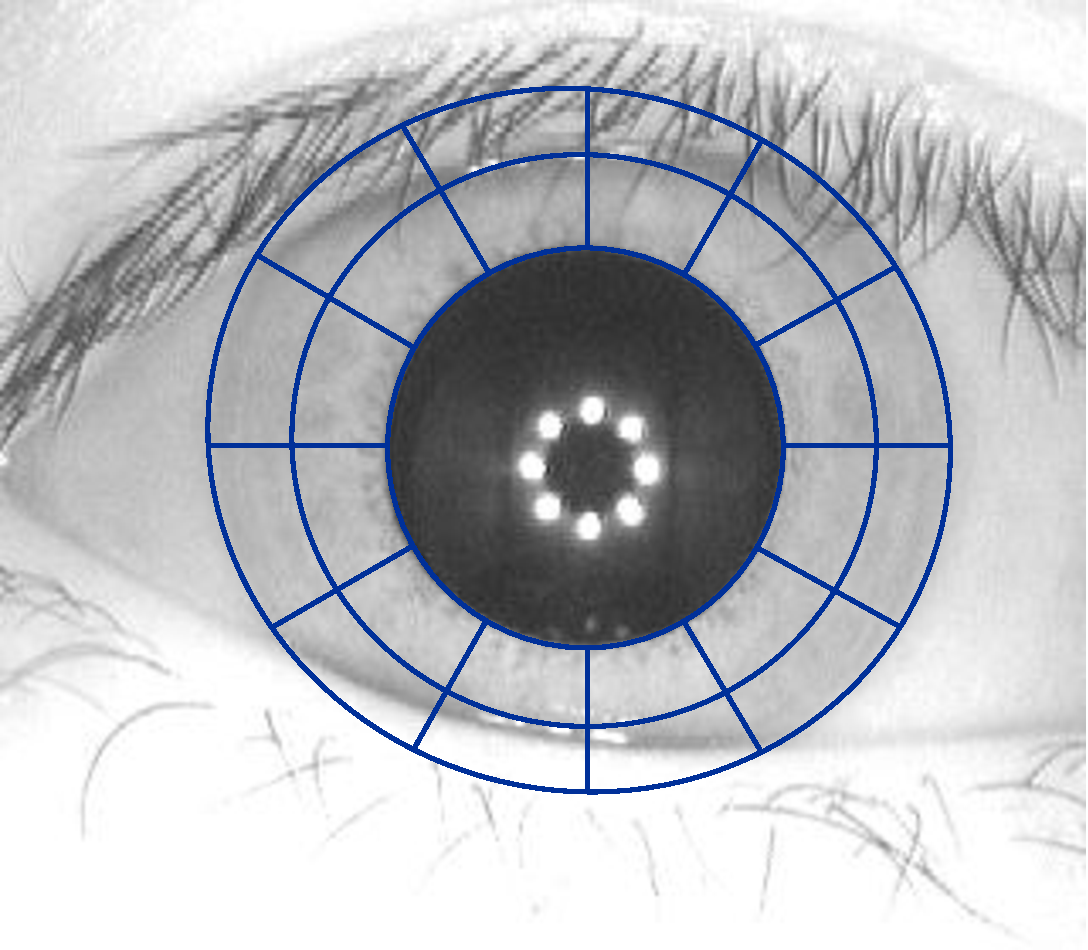
\includegraphics[width=0.6\linewidth]{figures/polar-image.pdf}
        \caption{The pupil and iris circumference ellipses define a polar coordinate system.}
        \label{fig:polar-method}
    \end{subfigure}
    \begin{subfigure}{0.5\linewidth}
        \centering
        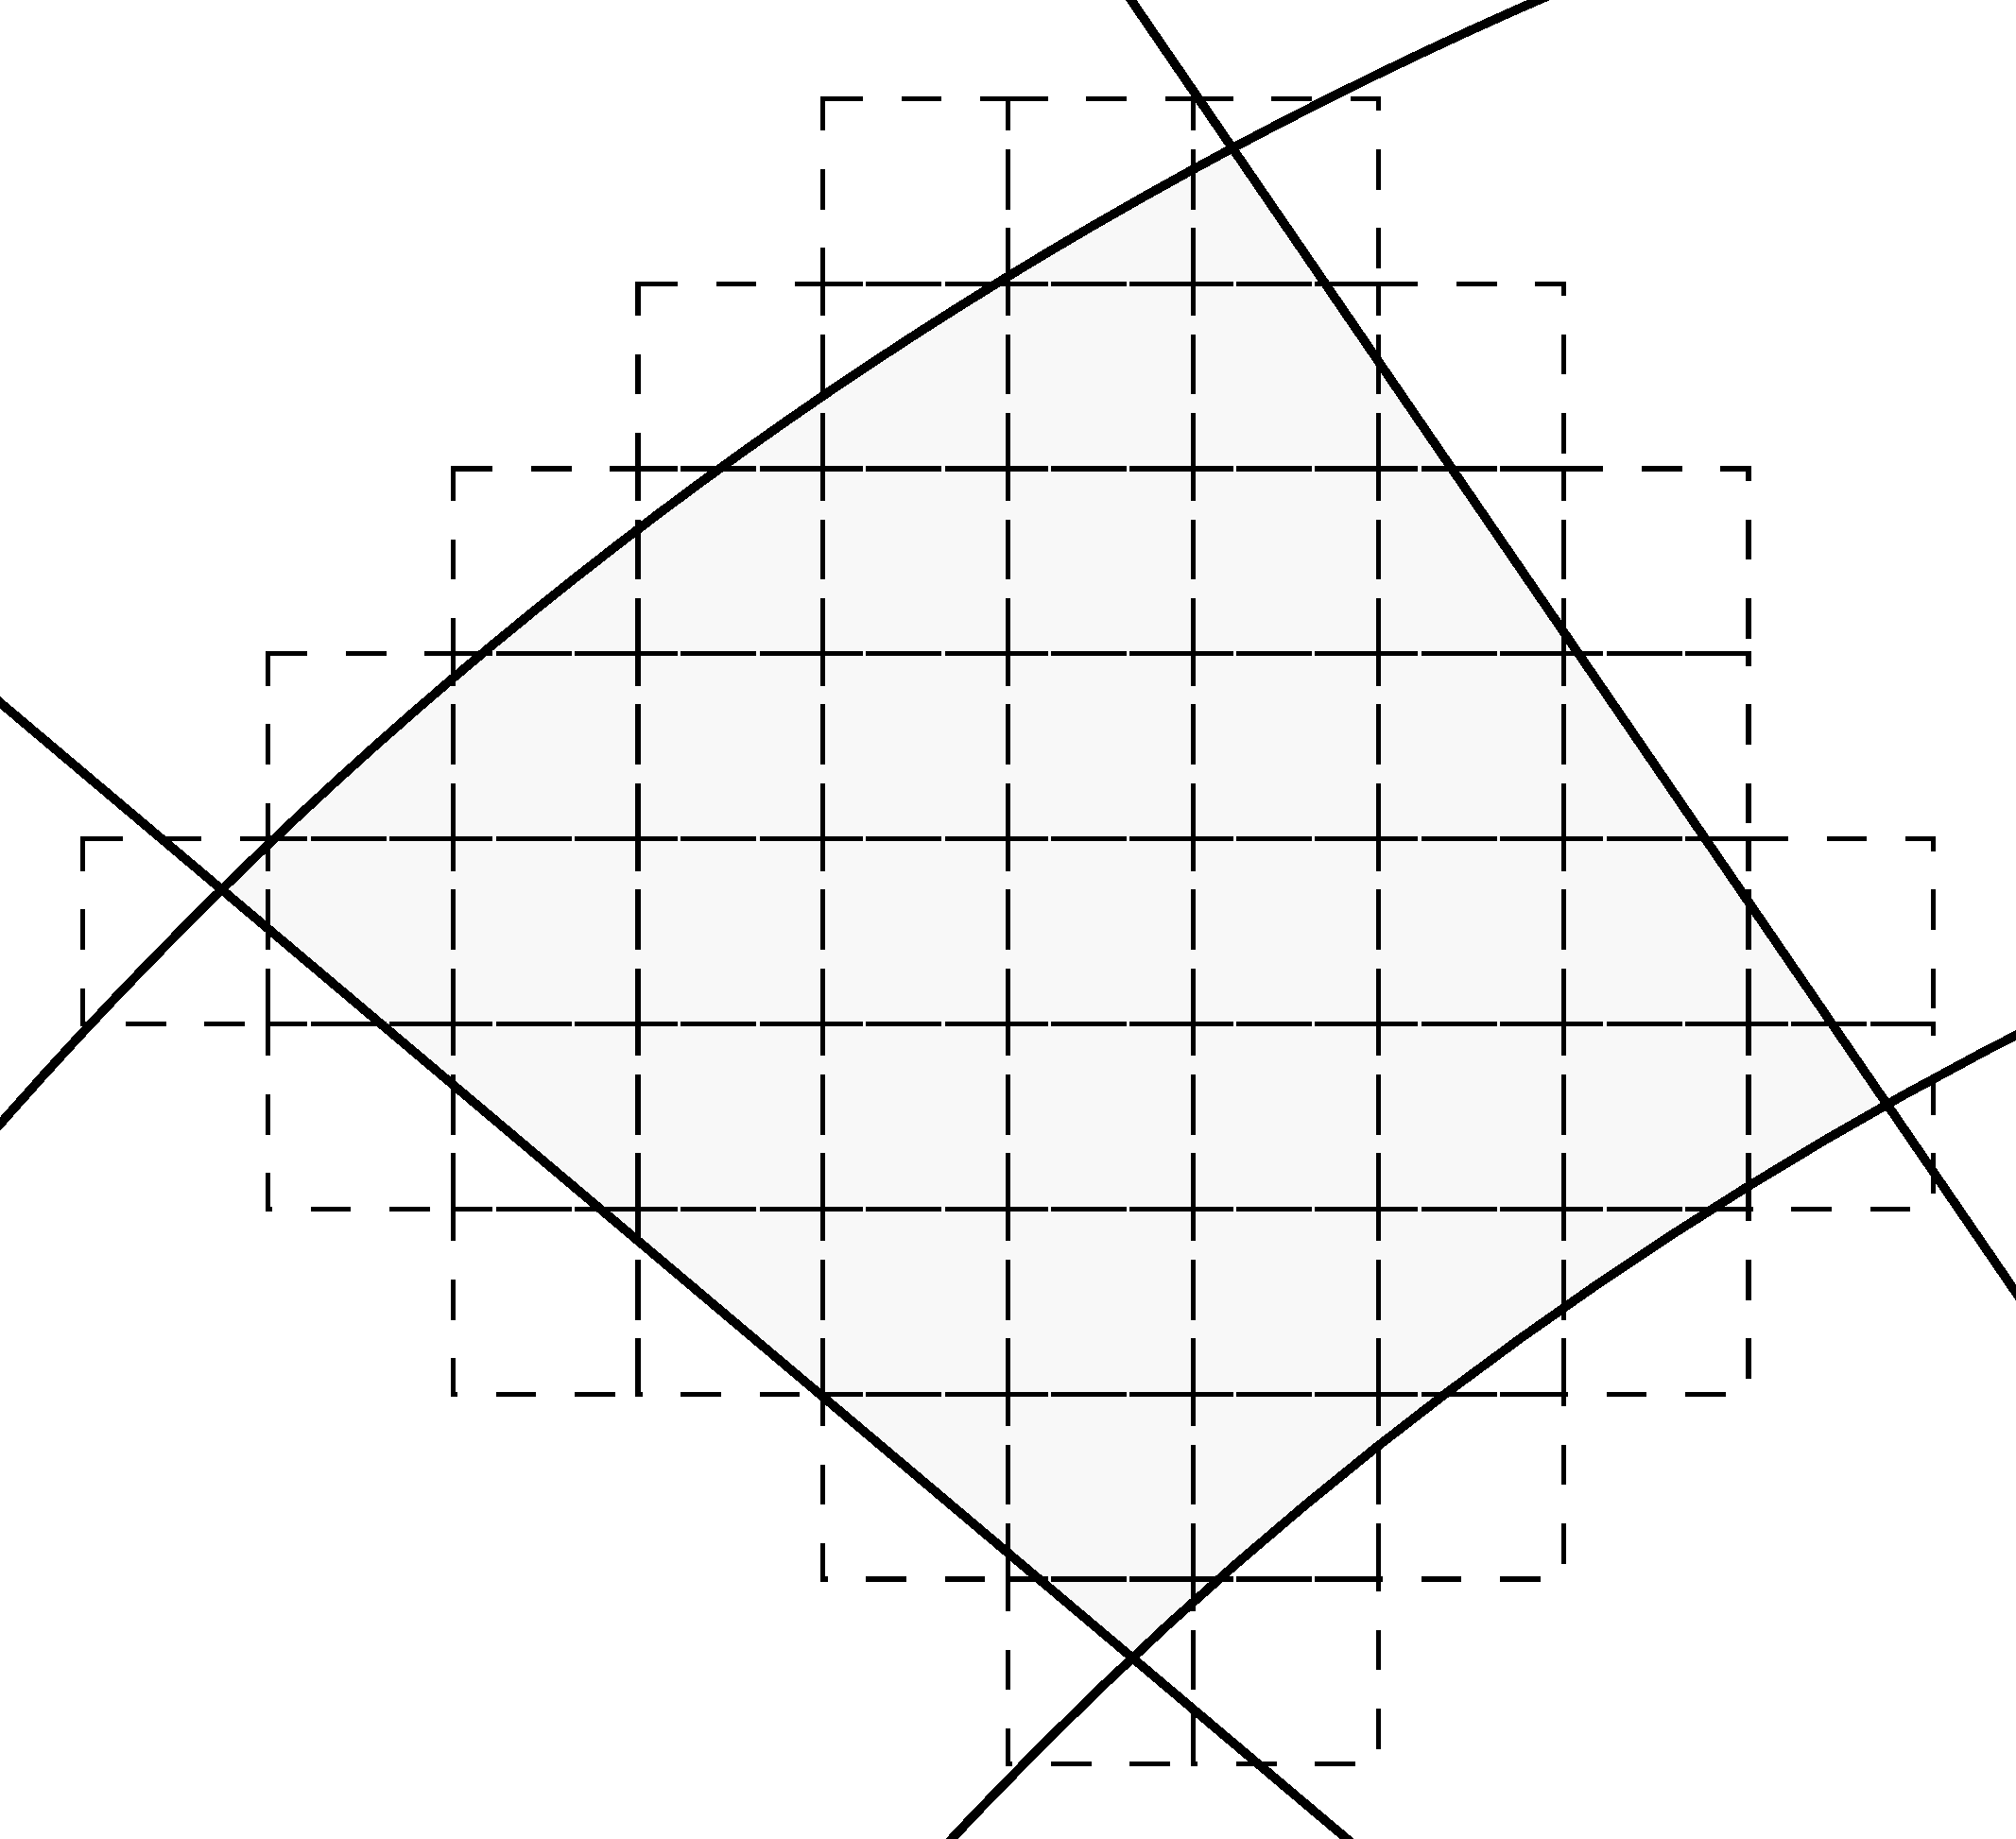
\includegraphics[width=0.6\linewidth]{figures/polar-method.pdf}
        \caption{Individual pixels in the polar coordinate system covers many actual pixels in the original cartesian space. The effect is amplified in the figure.}
        \label{fig:polar-method}
    \end{subfigure}
\end{figure}

The polar sampling method uses a particularly interesting technique. As shown in (FIGREF), the pseudo-polar coordinate system results in pixels that overlap several of the original image's pixels in strange ways. A possible solution would be to radically increase the polar resolution and use billinear sampling or similar for interpolation (REF). 

Due to the relatively slow phase calculation implementation however, I chose to keep the polar resolution low and instead opted to use a simple probabilistic sampling technique. If we denote the polar pixel region as a set $S$, each pixel in the cartesian image coordinate system is similarly sets $C_1, \dots, C_n$. The ideal pixel value at that coordinate is then:
\begin{equation}
    P(S) = \frac{\sum_{i=1}^n I_i A(S\cap C_i)}{A(S)}
\end{equation}

In other words, the pixel should take on the average value of the underlying pixels weighted by their intersecting areas. An easy way to implement this is by randomly sampling points inside $S$, adding their values, and dividing by $n$
\begin{equation}
    P(S) = \frac{1}{n}\sum_{x \sim U(S)}^n I_{x},
\end{equation}
where $U(S)$ is a uniform distribution over $S$. This method works for any size...

\begin{figure}
    \centering
    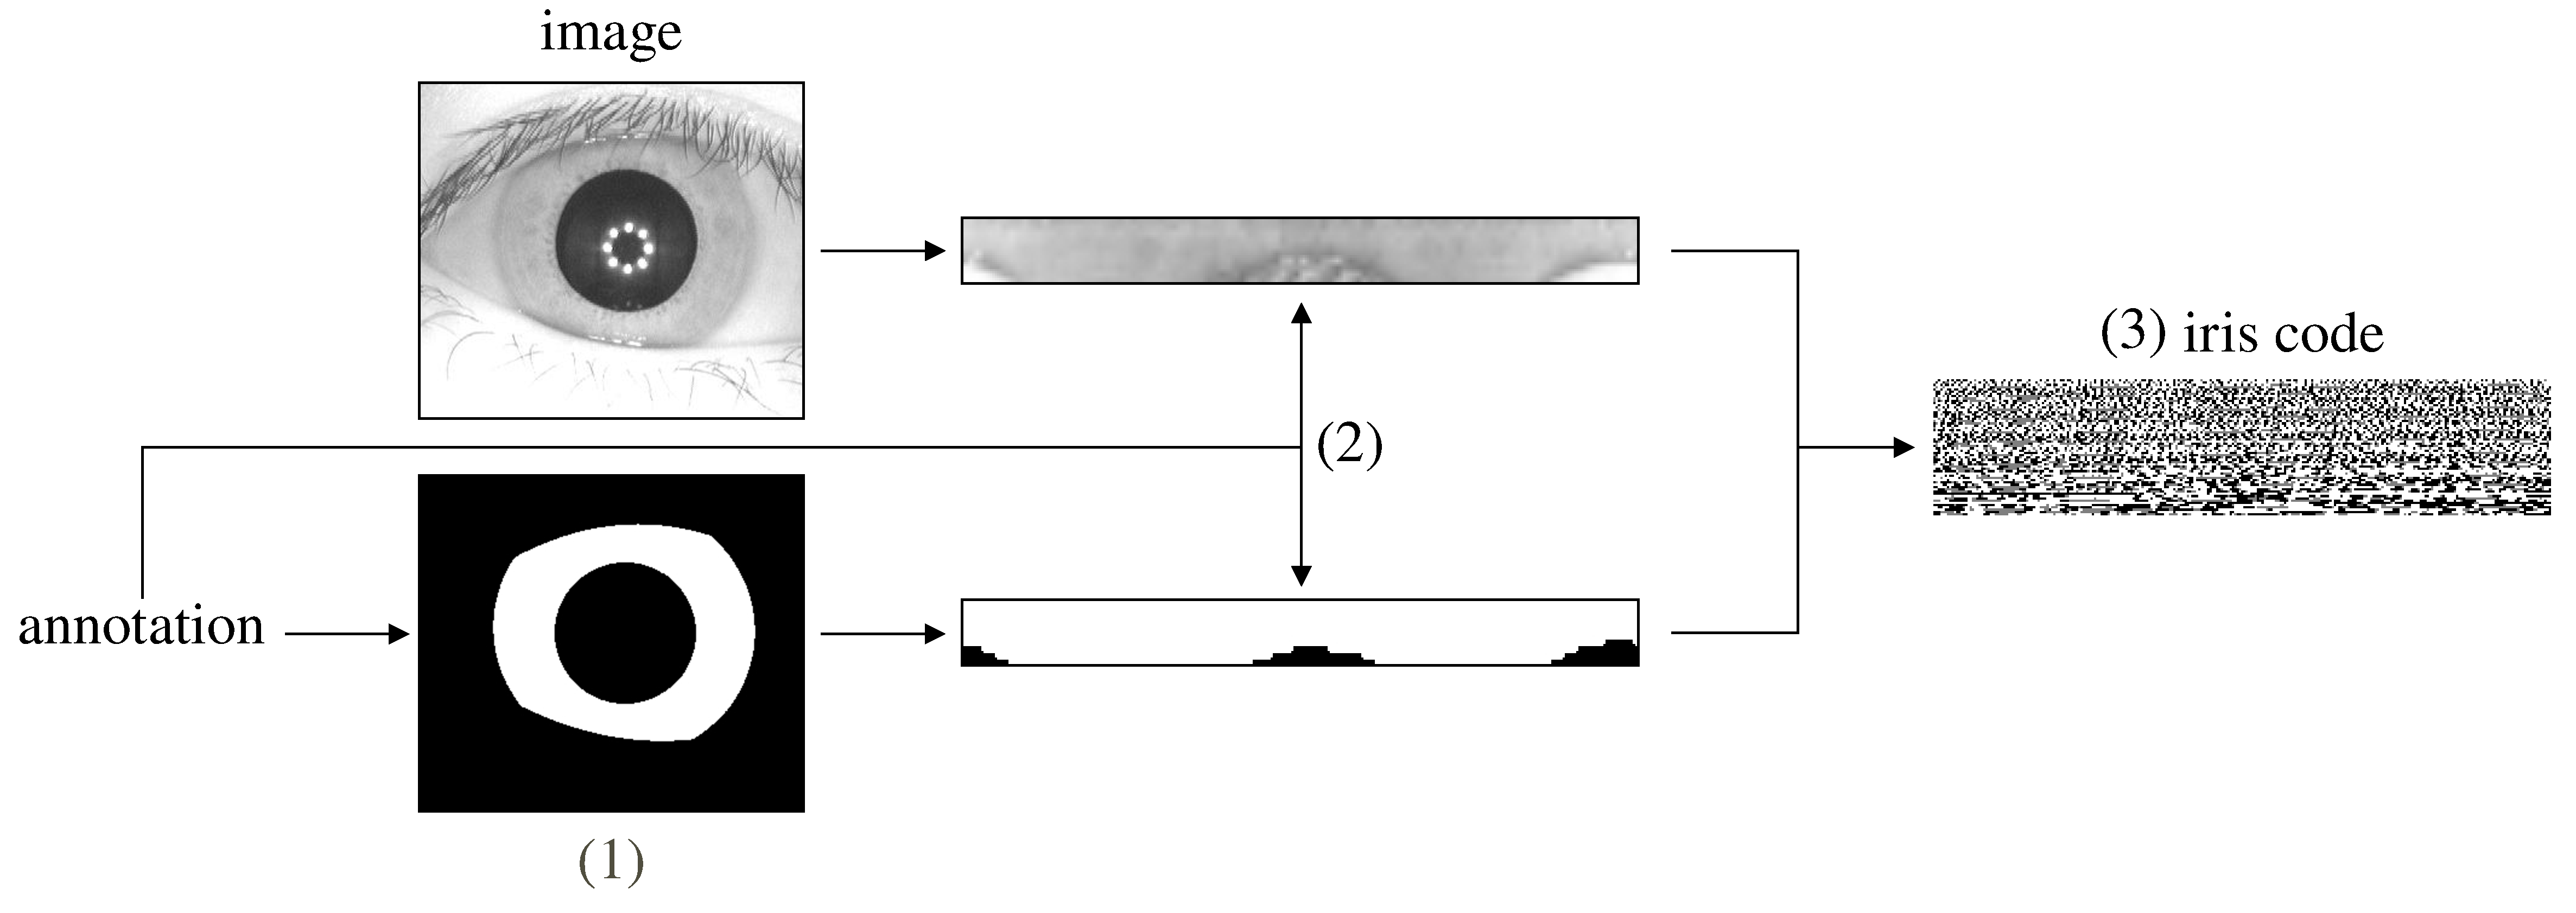
\includegraphics[width=1\linewidth]{figures/iris-code-gen.pdf}
    \caption{Iris code generation process. (1) The annotation (see text) is used to generate a binary mask of the visible parts of the iris. (2) The pupil and iris boundaries are used to create dimensionless polar projections of the iris and mask. (3) Gabor filters are applied to the polar image, quantized, and concatenated to a $16000$-element bit-vector which is the iris code. It is here visualised using black pixels for the value $0$ and white pixels for the value $1$. Pixels masked by the polar mask projection (and excluded from comparisons) are shown in grey (zooming might be necessary). }
    \label{fig:iris-code-gen}
\end{figure}

\section{Optimisation system}
Iris obfuscation has at least two objectives, one for the gaze accuracy and one for the iris recognition accuracy. This is problematic for classical optimisation where the goal is to find an extremum of a cost function with $\mathbb{R}$ as its domain. The field of multi-objective optimisation deals with exactly this kind of situation. A possible solution is to define a weighing of each sub-objective, i.e.
\begin{align}
	J^{\mathcal{O}}(I) = w_{gaze}J_{gaze}^{\mathcal{O}}(I) +  w_{iris}J_{iris}^{\mathcal{O}}(I),
\end{align}
as originally suggested by my supervisor in (REF). This approach may be suitable when sufficient knowledge about the problem makes it possible to define reasonable values for the weights. It does, however, assume prior knowledge of the relative importance of the objectives. 

Instead, this study focuses on exploring the trade-offs between various objectives over a large range of possible parameter values for each obfuscation method. In the article this is done using grid-search due to the relatively limited search space. I also experimented with a population-based method for combining multiple objectives which preserves (something).

A central idea in using these explorative methods is \textit{pareto optimality}. Pareto optimality is based on the concept that even when objectives are not comparable, it is possible to determine an ordering of the optimality of points. Figure (REF) shows an example in two dimensions. The points marked in blue are objectively better than any of the black points. Being objectively better here means that it is at least as good in every dimension and better in at least one. This is called dominance - the full definition is shown in \cref{def:dominance}. Points that are not dominated by any other point is \textit{Pareto optimal} (\Cref{def:p-optimal}). The subset of all such points of a given set is called the \textit{Pareto frontier} (\Cref{def:p-frontier}). In this example, the blue points define the Pareto Frontier.

\begin{definition}[Dominance]\label{def:dominance}
Given points $\mathbf{x}$, $\mathbf{x'}$ and an objective function $f$ with domain $\mathbb{m}$, $\mathbf{x}$ dominates $\mathbf{x'}$ if and only if
\begin{align}
 \forall i \in \{1, \dots, m\} :&\quad f_i(\mathbf{x})\leq f_i(\mathbf{x'}) \\
and \quad \exists i \in \{1, \dots, m\} :&\quad f_i(\mathbf{x}) < f_i(\mathbf{x'}).
\end{align}
In other words $\mathbf{x}$ cannot be worse than $\mathbf{x'}$ for any objective and has to be better on at least one.
\end{definition}

\begin{definition}[Pareto optimal]\label{def:p-optimal}
A point $\mathbf{x}$ in set $S$ is Pareto optimal if
\begin{align}
    \nexists \mathbf{x'} \in S: \quad \mathbf{x'} \text{ dominates } \mathbf{x}.
\end{align}
\end{definition}

\begin{definition}[Pareto frontier]\label{def:p-frontier}
The subset of all Pareto optimal points in a given set.
\end{definition}

Defining a Pareto frontier for a vector-valued objective function compresses the relevant parameter under consideration to a surface. This means that 

\begin{figure}
    \centering
    \begin{tikzpicture}
    
    \draw[thick,->] (0,0) -- (4,0) node[anchor=north west] {x axis};
    \draw[thick,->] (0,0) -- (0,4) node[anchor=south east] {y axis};
    
    \draw [red] plot [smooth cycle] coordinates {(1,1) (1,3) (3,3) (3,1)};
    \end{tikzpicture}
    \caption{Caption}
    \label{fig:my_label}
\end{figure}



\section{Filtering approaches}
We approach the analysis of separating the iris signal and the gaze signal from a pragmatic perspective. An image may be visualised as a height-map to more clearly display the individual pixel values. 

(FIG) shows an eye image and a one-dimensional slice where the light intensity is graphed as a function of the x-position. Clearly, the portion covering the iris shows relatively chaotic changes but low variance compared to the rest of the image. The pupil-iris boundary and glint-pupil boundary which are used in our gaze-estimation method are clearly identifiable since they are represented as huge changes in intensity. These sorts of examples are typically also shown when introducing image edge detection, since it clearly demonstrates the connection between rate of change, i.e. the gradient, and the presence of an edge. 

When analysing the image as a Fourier series, two important factors stand out. Firstly, the iris seems to be dominated by a low-amplitude, very random signal. This indicates a range of small to medium wavelengths and high entropy. The edge regions, which are used by our gaze algorithm, instead look roughly like square waves. A square wave requires an infinite Fourier series to be represented accurately. Because the image is effectively band-limited, it is possible to recreate it with a finite series but it still spans the whole wavelength spectrum.

This signal analysis becomes important when considering methods for obfuscation. Our understanding of how the transformations affect different simpler signals may help us find suitable methods that are more well-suited to the application.

\subsection{Measuring information in images}
The term signal is rather abstract but is typically defined as a function that encodes or contains information of interest. Signals can be defined over temporal inputs, spatial inputs, or both. In the case of eye information processes, signals such as the captured eye images may be analysed individually as purely spatially divided signals or jointly as a time series of frames. The iris pattern in either its abstract or encoded form, is only resolved spatially while the gaze signal is usually analysed as a time-series. 




When viewed as bandlimited discrete signals of two dimensions, images can be analysed structurally through the 

To measure entropy and mutual information in images, it is necessary to formulate a method for defining the image in terms of a probability distribution. Specifically, it is necessary to define a model for the image distribution and estimate it using the image itself as data.

The fundamental model is that each image can be represented by an unknown distribution $P_{img}$ of an unknown number of random variables $X^1, \dots, X^n$. A simple model is the intensity histogram which estimates a discrete distribution of intensity values assuming that each pixel is independent of each other. It can be defined as
\begin{align}
    P(I=i) = \sum_{x\in\mathcal{X}y\in\mathcal{Y}} \delta_{i, I_{x,y}},
\end{align}
where $\delta_{a, b}$ is the Dirac delta function. The downside to this approach is that no correlations between pixels are considered even though they clearly exist. For use in obfuscation measurement, this is problematic since the iris recognition methods use texture and not direct pixel intensities for detection. 

In the most general terms, the distinct features of an iris pattern represents differences in the amplitude and phase of different frequencies. Many iris algorithms of the Daugman type use spatial phase responses to calculate a robust iris code. These traditional methods generally use some form of wavelet transform to separate spatial frequency-responses (REFS). The convolutional neural-network based methods likely learn similar approaches as they have been shown to learn typical bandpass-filters like the wavelets used by Daugman (REF). 

The image derivative, defined by its two partials, has excellent properties for measuring image texture complexity. The image derivative retains all information necessary to reconstruct the original image and is therefore still a valid upper bound on information measures (REF). By defining $P_{img}$ as a joint distribution of the partial derivatives of the image
\begin{align}
    P(dx=i, dy=j) = \sum_{x\in\mathcal{X}y\in\mathcal{Y}} \delta_{i, {I_{\Delta x}}_{x,y}} \delta_{j, {I_{\Delta y}}_{x,y}},
\end{align}

Additionally, we also define joint distributions on convolutions with complex Gabor wavelets. A Gabor wavelet works as a bandpass filter, i.e. it responds only to certain frequency ranges. Defining a joint distribution over the Gabor response of a particular filter makes it possible to measure the entropy in certain frequency ranges which further... By definition however, a bandpass filter does not retain all the information in the original signal and can therefore not be used for definition of upper bounds.




\subsubsection{Filters}

\begin{figure}
    \centering
    \includegraphics[width=1\linewidth]{figures/filter_effect.pdf}
    \caption{Shows effect of applying the proposed filters. The heat-maps show the corresponding gradient histogram.}
    \label{fig:filters}
\end{figure}
Specifically, one of the previous studies tested a Gaussian filter (and optical defocus) (REF) for obfuscation based on the assumption that the lowest frequency wavelength of the pupil edge would be enough to enable robust gaze estimation. The problem with the Gaussian filter is that it is a low-pass filter, i.e. it removes high-frequency components. Since sharp edges are only sharp because of these, a Gaussian filter makes images look blurry and unsharp as a result. The effect on the image in (FIG) is shown in (FIG), where a Gaussian filter with $\sigma=5$ has been applied. Clearly, the gradient at the edge has been smoothed considerably. The reason the study still reports favourable results is that the gaze-estimation algorithm is likely robust to at least some degree of edge blurring.

A smarter approach is to consider not just the spatial neighbourhood but the intensity as well. 

\chapter{Discussion}
This chapter is an extension to the article with additional analysis of the results and a more thorough discussion of how the results support the proposed model and what insights the results give to support its use for other applications.

\section{A detailed look at obfuscation method information}
\begin{figure}
	\centering
	
	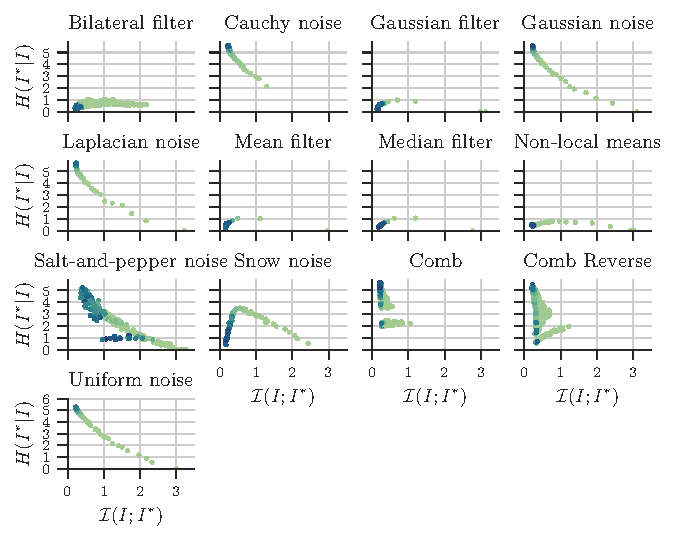
\includegraphics[width=1\textwidth]{figures/results/individual}
	
	\caption{Plot of mutual information and conditional information response for individual filters. Note that these distributions are estimated from the entire image, producing less noisy results than the ones presented in the article.}\label{fig:individual}
\end{figure}

\Cref{fig:individual} shows mutual information and conditional entropy for each filter separately. This makes the distinction between them even more noticeable. 

The noise methods, except snow and salt-and-pepper, all follow an almost straight line, "converting" mutual information into conditional entropy. \Cref{fig:individual-entropy} is similar, but with the output image entropy as its x-axis. From this figure it is clear that for all noise methods, the increase in conditional information is roughly proportional to the increase in entropy, but not at a one-to-one scale. As shown in \cref{eq:entropy-law}, this necessitates a loss in mutual information, i.e. $\mathcal{I}(I^*;I) = H(I^*) - H(I^*|I)$. Since the entropy and conditional entropy are roughly linearly correlated for the noise-based methods, we have $H(I^*) \approx \alpha H(I^*|I) + H(I)$ and as a consequence, the mutual information can be expressed as a function of the conditional entropy and the entropy of the original image 
\begin{align*}
\mathcal{I}(I^*;I) \approx (\alpha-1)H(I^*|I) + H(I).
\end{align*}
This is of course only an approximation.

The snow method has a sudden drop in conditional information which is caused by its definition. At low densities, snow increases conditional entropy because the randomly placed pixels adds high gradient components. At higher densities however, the fact that only the value $127$ is used for pixels starts to decrease the entropy significantly. %The uniform snow method is susceptible to the same effect when gaussian variance is low and \todo{what about this?}

\begin{figure}
	\centering
	
	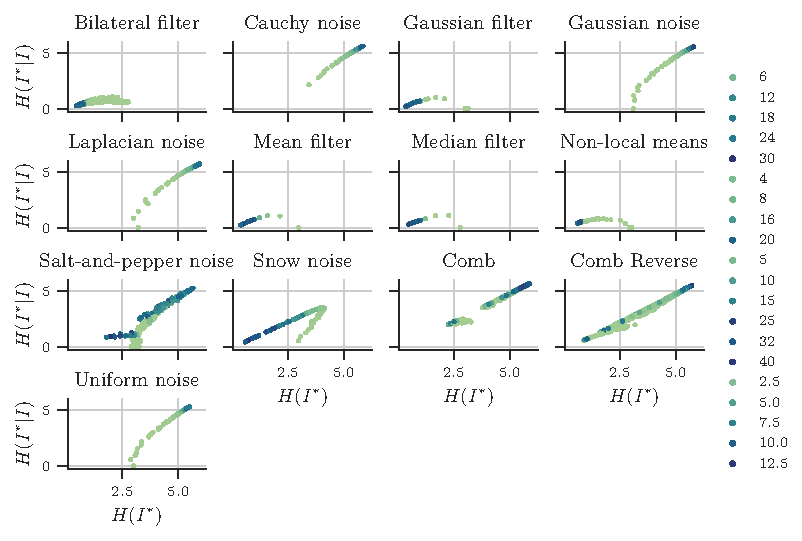
\includegraphics[width=1\textwidth]{figures/results/individual-ent}
	
	\caption{Plot of entropy of the obfuscated images and conditional information response for individual filters.}\label{fig:individual-entropy}
\end{figure}

The filter-based methods behave as explained in the article and mainly impact mutual information. The combination methods, and especially Comb, is worth investigating further. \Cref{fig:comb} uses the same axes as \cref{fig:individual} but displays only data from the Comb method and with the colours indicating the three parameters in the respective plots. The scale parameter, $\gamma$, correlates directly with the value of conditional entropy as expected. The generally lower mutual information values are likely caused by a narrower band of parameters used for the experiment due to time considerations. It shows that the diagonal bands visible in the figures corresponds to the response caused by the bilateral filter. It correlates highly with the color variance parameter $\sigma_c$ but is seemingly independent from the spatial parameter $\sigma_s$. This effectively means that only small values of $\sigma_s$ is needed.

\begin{figure}
	\centering
	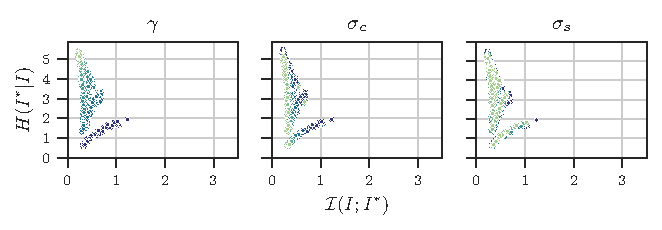
\includegraphics[width=1\textwidth]{figures/results/comb}
	\caption{}\label{fig:comb}
\end{figure}
\todo{Discuss camera effects}

\subsection{Filters and gradient entropy}
Although the approach to filtering has been argued extensively in the article, it did not show how visually appropriate the gradient entropy is compared to a simple intensity entropy. \Cref{fig:delentropy} shows a number of sample images for which both the intensity histogram and gradient histograms have been calculated. It is visually very clear how the gradient histogram and its entropy corresponds with the visually perceived image complexity.

\begin{figure}
    \centering
    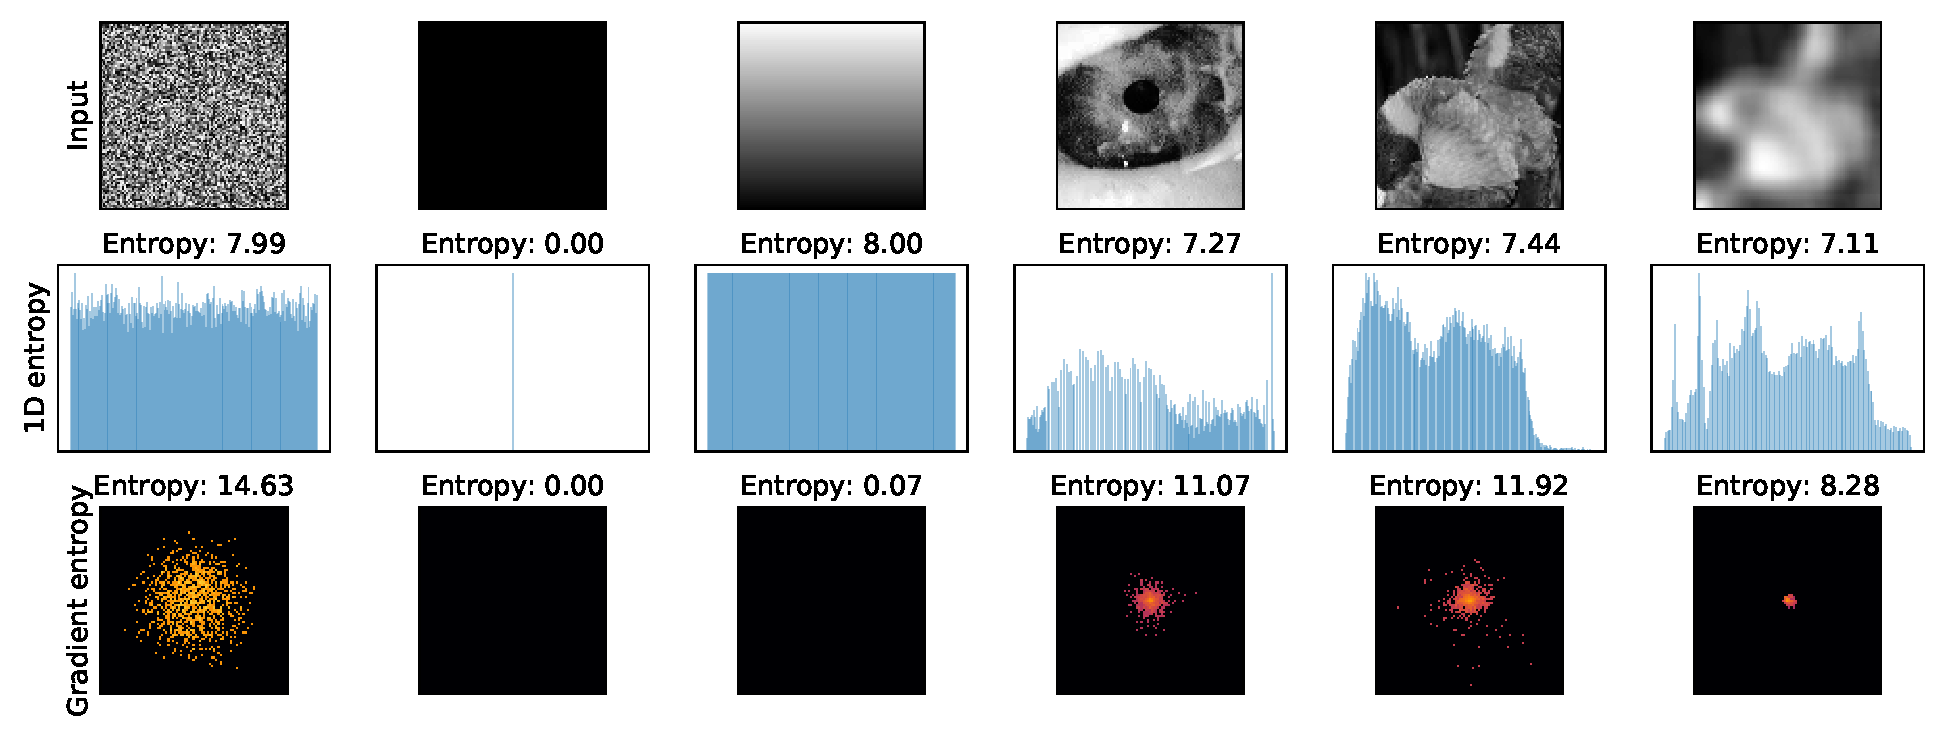
\includegraphics[width=1\linewidth]{figures/results/delentropy}
    \caption{Comparison between entropy of intensity and gradient histograms for a number of image samples.}
    \label{fig:delentropy}
\end{figure}

Sample applications of the proposed obfuscation methods are shown in \cref{fig:filters} where the same visual correlation is still clearly present. The Comb method is also visually indicative of its effectiveness as an obfuscation method because of the clear blurring of eye details while retaining a layer of noise. The parameters used in this example are exaggerated to increase the perceivability of the effects.

\begin{figure}
    \centering
    \includegraphics[width=0.85\linewidth]{figures/results/filter_effect.pdf}
    \caption{Shows effect of applying the proposed filters. The heat-maps show the corresponding gradient histogram.}
    \label{fig:filters}
\end{figure}


%Specifically, one of the previous studies tested a Gaussian filter (and optical defocus) \parencite{BRENDAN_BLUR} for obfuscation based on the assumption that the lowest frequency wavelength of the pupil edge would be enough to enable robust gaze estimation. The problem with the Gaussian filter is that it is a low-pass filter, i.e. it removes high-frequency components. Since sharp edges are only sharp because of these, a Gaussian filter makes images look blurry and unsharp as a result. The effect on the image in (FIG) is shown in (FIG)\todo{do it}, where a Gaussian filter with $\sigma=5$ has been applied. Clearly, the gradient at the edge has been smoothed considerably. The reason the study still reports favourable results is that the gaze-estimation algorithm is likely robust to at least some degree of edge blurring.

%A smarter approach is to consider not just the spatial neighbourhood but the intensity as well. 

\section{Eye information process model generalisation}\todo{ikke klart hvem der siger det...}
For the model and methodology presented in this thesis to be useful, it has to be relevant to the way this category of problems are perceived and to how they are evaluated. For the specific application of iris obfuscation, this has been argued extensively in the article. At an abstract level, the model is used to understand the problem of iris obfuscation and for proposing reasonable and interesting solution candidates. At a concrete level, the information-based metrics and methods derived for calculating them for images showed a high correlation with the observed iris recognition accuracy.

The definition of the model itself as a Bayesian network or as a communication system is an expression of the similarity of image and signal manipulation operations and, by extension, of obfuscation methods in general. The optimisation goal defined for iris obfuscation is thus the same for any other obfuscation problem. The gaze signal itself contains information that has been shown to reveal multiple properties of the recorded subject and is therefore an obvious candidate for using the model. The model and methodology presented here can be applied directly. 

If applied to other problems, results become easier to analyse and compare, and the methodology itself will develop which might provide additional insight into already published material. 

\section{Differential privacy}
Differential privacy is too strict to be a realistic measure for proving privacy bounds for obfuscation tasks. Specifically, only low privacy-bounds are achievable by the application methods proposed so far in the literature. I here present the argument that this is caused by the properties of differential privacy when applied in this domain. Differential privacy is simply a measure of how much a random function impacts the predictability of changing a single element in a set of data points, e.g. an image. Formally, a random function $\mathcal{K}$ is $\epsilon$-differentially private if
\begin{align}
	P[\mathcal{K}(D_1)\in S] \leq \exp{\epsilon} P[\mathcal{K}(D_2)\in S],
\end{align}
for all subsets $S$ of the image of $\mathcal{K}$ and all datasets $D_1$, $D_2$ that differ in at most one element \parencite{dwork2006differential}. In other words, a differentially private function decreases the output's dependence on individual data points since this dependence can be used to infer the original data points.

Differential privacy measures for images have been proposed by \parencite{fan2018image}. Importantly, their extension from single pixel changes to neighbourhoods come with a proportional increase in $\epsilon$ for the same amount of randomness, i.e. for a neighbourhood of $n$ pixels, the privacy should be $\epsilon/n$ to achieve the same level of protection as when a single element is changed. The solution presented in this study suggests an aggressive downsampling using averaging to achieve reasonable levels of noise. Specifically, for an image with pixel intensities in the range $0-255$, and using laplacian noise, the scale parameter is $\frac{255n}{b^2}$ where $b$ is the side length of grid cells defining regions to be averaged. Since laplacian noise has a variance of $2s^2$ where $s$ is the scale, even a low-resolution image of $100\times 10$ pixels (the size used for polar iris images in this work) would require laplacian noise with a variance of $\approx 130\times 10^9$ thus rendering the image practically unusable.

The method proposed in \parencite{BRENDAN_SNOW} does, however, use a weaker form of differential privacy allowing an extra constant term $\delta$ which signifies a probability of leaking information. They prove that $\delta$ has a maximum of $0.5$ for the snow method which means that each pixel has $50\%$ chance of a leak. However, as presented in \cref{sec:methods}, the method can easily be defeated if multiple samples are available. Additionally, even with a single sample, the method shows only moderate effectiveness at preventing recognition with high precision at low recall values. 

In conclusion, differential privacy is not suitable for determining the security of obfuscation methods due to their high sensitivity and the large areas of pixels that need to be secured. As a final note, this criticism does not concern the aggregation based attempts at differential privacy in eye-tracking mentioned in the article. %Instead it is 
 differential privacy has been shown to be highly effective in other eye-tracking privacy tasks where aggregation is involved \parencite{differential-general, differential-general-two}.

\todo{Try to add the rest here}
% Instead, definitions should be derived from a

%\begin{definition}[Privacy]
%Let $S$ be an eye information signal and $\bar{S} \subseteq S$ a subset describing the sensitive data. 

%Let $\mathcal{A}$ be an arbitrary function for inferring 
%Given an arbitrary information extraction function $\mathcal{A}$, an obfuscation function $\mathcal{O}$, and a signal $S$, the privacy strength of $\mathcal{O}$ is defined as
%\begin{align}
%	P[\mathcal{A}(\mathcal{O}(S)) \cup \bar{S} \neq \empty] \leq \rho,
%\end{align}
%for an arbitrary threshold $\rho$ and for any $\mathcal{A}$.
%\end{definition}

























\chapter{Future work}
As suggested throughout the thesis, the EIP model and the surrounding work is meant to be an offset for future work in the area of sensitive information removal in eye-tracking. The large number of personally sensitive properties eye-tracking data potentially reveals is a problem that needs to be investigated further. This chapter presents my thoughts on the most critical issues and what solutions might be achievable using the approach presented here.



\section{Iris obfuscation}
Iris-obfuscation is, as mentioned, a good place for foundational research due to the fact that it enables other discovered properties to be linked to an identity with extremely high precision given high-resolution data as is typically recorded with head-mounted eye-trackers. The results presented shows that the proposed model combining blurring and noise generation might be a promising solution. It is however extremely important, that these and other methods are studied in even greater detail to provide better guarantees for their security. 


\subsection{Finding strict boundaries}
I propose to continue pursuing information-related measures as a basis for proving iris obfuscation methods secure. A reasonable starting point is to use the mutual information as well as its ratio to the total entropy of the iris pattern in the image. Alternatively, the capacity measure can be used to define theoretical upper bounds that are not dependent on specific data.

The histograms used in these experiments use only 16 bins per dimension which itself removes a lot of information. The resulting values are therefore not representative of the true entropy of the images. Since this is limited by the number of samples, using a whole dataset as a single signal to estimate the distribution will make it possible to more accurately approximate the true distribution. Other approaches such as kernel density estimation might be used as well.

\subsection{Efficient parameter optimisation}\label{sec:future-optim}
As mentioned in \cref{sec:detail-opt}, a vector evaluated genetic algorithm has been implemented as part of the optimisation system. A vector evaluated genetic algorithm is a simple variation of a traditional genetic algorithm with a selection criteria, crossover, and mutation steps as defined in \parencite[148, 222]{kochenderfer2019algorithms}. Instead of selecting a number of parents based on a single selection criteria, the vector algorithm divides the population into subpopulations which are each optimised (selection) according to a specific output feature. The result is that all measures are considered. 

Due to time constraints and the relative effectiveness of the brute-force grid-search, this implementation was never adequately tested but might be useful, especially for methods with higher numbers of parameters. The Comb and Comb-reverse methods are interesting candidates for this approach due to them having three parameters.

\subsection{Learning iris obfuscation}
Applying neural network methods to learn the obfuscation functions from data has two purposes. (1) Given the success of neural networks in other areas of computer vision, it is reasonable to expect that an obfuscation method trained from data would be better adapted to the task than the methods presented here. (2) The learned models can be analysed to better understand how iris obfuscation can work.

\subsubsection{A possible model}
One of the original goals for this thesis was to create a simple CNN model for iris obfuscation. This section contains my thoughts for a definition. Neural networks are an ideal model for this application since they allow optimisation of arbitrary functions. This means that complex priors and methods for measuring cost can be implemented easily. 
%Neural networks are just differentiable functions which are optimised using stochastic gradient descent. The stochastic modifier signifies, that instead of determining the true gradient, a smaller sample is used instead, resulting in realistic time-frames for optimisation. Although neural networks are often described by layers and neurons, this terminology is all a combination of the history of their creation and useful architectural terms. In general, we may model any function as long as it can be differentiated.

For iris obfuscation, an important characteristic is effectiveness since the method should work in an embedded environment either as software or hardware. Locality and depth are therefore important considerations for the design of a neural network for iris obfuscation.

Because both the input and output are images, the architecture should be a fully convolutional network (FCN) which contains no linear layers. This allows the "field of view" of each pixel to be limited by the radius
\begin{align}
    neigh = (k-1)/2*L,
\end{align}
where $k$ is the kernel size and $L$ is the number of layers. 

The gradient-based entropy measures are an ideal candidate for measuring the degree of obfuscation in an image since it is differentiable. Alternatively, neural-network based iris recognition models may be used \parencite{nguyen2017iris, gangwar2016deepirisnet} but they introduce method-specific biases that may or may not be acceptable. Additionally, the measures presented in the article are shown to correlate highly with the iris recognition accuracy.

%Redefining the measures as differentiable functions require a histogram binning method that is continuous. A method proposed in \parencite{avi2019hue} is extended to be usable for multivariate distributions. 
%
%The traditional histogram counting function is defined as
%\begin{align}
%	h(v) = \sum_{x\in I} \delta_{I_x, v},
%\end{align}
%which is not continuous. Instead, the counting function is substituted with 
%
%\begin{align}
%    \Pi_k(z) = \sigma(\frac{z-\mu_k+L/2}{W}) - \sigma(\frac{z-\mu_k-L/2}{W})
%\end{align}
%
%\begin{align}
%    P_I(k) = \frac{1}{N}\sum_{x\in\Omega}\Pi_k(I(x))
%\end{align}
%
%\begin{align}
%    P_{\nabla I}(\partial x, \partial y) = \frac{1}{N}\sum_{x\in\Omega}\Pi_{\partial x}(I(x))\Pi_{\partial y}(I(x)) = \frac{1}{N}P_{\partial x}P_{\partial y}^T
%\end{align}
%
%\begin{align}
%    P_{\nabla I_1, \nabla I_2}(\partial x_1, \partial y_1, \partial x_2, \partial y_2) = \frac{1}{N}\sum_{x\in\Omega}\Pi_{\partial x_1}(I(x))\Pi_{\partial y_1}(I(x))\Pi_{\partial x_2}(I(x))\Pi_{\partial y_2}(I(x))
%\end{align}
%
%\begin{align}
%    J(\nabla I_1, \nabla I_2) = \frac{1}{N}P_1P_2^TP_3P_4^T
%\end{align}
%
%\begin{figure}
%    \centering
%    \begin{tikzpicture}
%    \begin{axis}
%    \addplot[
%        samples=100
%    ]
%    {1/(1+exp(-x)};
%    \end{axis}
%    \end{tikzpicture}
%    \caption{Caption}
%    \label{fig:my_label}
%\end{figure}
%
%
%\begin{align}
%    J(\theta) = \frac{1}{2}\mathbb{E}_{x,y\sim \hat{p}_{data}} ||\mathbf{y}-f(x;\theta)||^2
%\end{align}
%
%\begin{align}
%    Z_{i,j,k} = \sum_{l,m,n} V_{l,j+m-1, k+n-1}K_{i,l,m,n}
%\end{align}


\todo{kun hvis du kan nå det!!}

\subsection{Combined training}
I propose that training a complete gaze estimation pipeline as neural network with a dedicated iris obfuscation component is an obvious next step for exploring how the iris and gaze signal components in images might be modified in a manner that is beneficial to both iris obfuscation and gaze estimation. In other words, I suggest the possibility of improving neural-network based gaze estimation by jointly training a network for iris obfuscation and gaze estimation. Although the encoded iris is clearly indicative of the eye's position and rotation and thus usable for gaze estimation, a jointly trained method may selectively retain important features for gaze while removing noise and iris pattern information.







\chapter{Conclusion}
This thesis has presented the concept of an eye information process as a building block for understanding how information is stored in eye tracking data and how different source signals may be selectively degraded by applying obfuscation techniques that exploit specific characteristics of a target signal. This idea makes it possible to redefine eye information process tasks such as gaze estimation and iris recognition using the same terminology. This makes it possible to investigate the interactions between different EIPs using the same theoretical framework and create concepts for information obfuscation that do not depend on specific definitions of individual processes.

Iris obfuscation is used as the focus for the presented experimental work due to the high accuracy of existing recognition methods. Two experiments are proposed to comprehensively test both possible optimisation of method parameters and precise obfuscation performance. A number of new method proposals all outperform existing methods with the proposed method Comb showing by far the best performance. The study is thus meant as the first proper overview of the iris obfuscation problem and how it might be solved. It is also a proposal to use the EIP model for formulating more general problems and work towards strict notions of the obfuscation performance that provide theoretical guarantees instead of only empirical ones.

I propose a number of interesting directions for future development. Using CNNs for iris obfuscation (as proposed by my supervisor) may lead to further analyses of how simple obfuscation methods might work and may be used in the creation of full end-to-end gaze-estimation pipelines using neural networks that implement obfuscation implicitly. Another direction is the use of EIP model and surrounding methodology of obfuscation to EIPs using gaze for information extraction. This use-case is interesting because the information that may be extracted from gaze is very sensitive if identification is possible. Finally, the existing use case and approach (iris obfuscation using simple filters or noise generators) can be improved by automatic parameter optimisation methods and exploration of strict definitions for security using the proposed information measures.

%Eye-tracking is becoming increasingly prevalent due to reductions in production costs and advances in technology and software. Because the human eye can be used to infer different sensitive properties including identity, security and privacy research in eye-tracking is highly relevant. Because the data used in eye-tracking systems contains sensitive information, methods that selectively obfuscate sensitive information need to be developed.


%Security and privacy in eye-tracking are therefore highly relevant areas of research as the potential for abuse or leakage of sensitive 
%Security and privacy in eye-tracking is becoming increasingly important because 


%* A model for understanding eye information
%* A discussion about the importance of defining a common framework for obfuscation.
%* A comprehensive test of iris obfuscation methods
%* A novel method for iris obfuscation that performs very well

%This goal of this project was to look into the question of how sensi- tive information can be removed from eye-tracking processes while retaining utility. Specifically, I investigated how machine learning might help create optimal models for doing so. This led to three sub- questions that I have tried to answer to various degrees. A summary of the answers are presented here in order:
%1. I have presented an overview of the anatomy of eyes as well as the field of eye-tracking and current methods for personal identification using eye-information. This leads me to propose a simple classification scheme for information in eye-trackers. This scheme can be used to easily compare and understand dif- ferent information-related issues in eye tracking.
%2. I have presented a proposal for how sensitive information can be removed without making a negative impact on utility for the specific case of iris-recognition. The proposal is based on general information theory as well as specific methods for iris- recognition. The prototype uses a bilateral filter optimised using random-search to remove iris-information from eye images. The result was a very minor impact on pupil detection accuracy. It is a promising method that deserves further examination.
%3. For security, I presented delentropy as a general measure of in- formation content in signals of highly correlated values such as images. Although it empirically reflects visual degradation of iris-patterns, further testing is needed to assert its actual use- fulness. Additional measures may have to be considered. For utility, the best method may be to test archetypical gaze estima- tion systems for a wide coverage of methods.

\printbibliography

\newpage

\printnoidxglossaries
\printnomenclature[1in]

\newpage
\appendix
\chapter{Parameter tables}
\begin{table}[]
    \centering

    \begin{tabular}{llllllll}
\toprule
              &               &           &       &        &       &    &    \\
Type & Filter & Parameter & start & stop & num & step & val \\
\midrule
Constant & Gaussian noise & $\mu$ & NA & NA & NA & NA & 0.0 \\
\cline{2-8}
\multirow{2}{*}{Increments} & Mean filter & Kernel size & 1.00  & 51.00  & NA & 2.0 & NA \\
\cline{2-8}
              & Median filter & Kernel size & 1.00  & 51.00  & NA & 2.0 & NA \\
\cline{1-8}
\multirow{17}{*}{Interpolation} & \multirow{2}{*}{Bilateral filter} & $\sigma_c$ & 5.00  & 100.00 & 30.0  & NA & NA \\
              &               & $\sigma_s$ & 1.00  & 20.00  & 30.0  & NA & NA \\
\cline{2-8}
              & Cauchy noise & $\sigma$ & 1.00  & 50.00  & 100.0 & NA & NA \\
              \cline{2-8}
              & \multirow{3}{*}{Comb} & $\sigma$ & 1.00  & 50.00  & 20.0  & NA & NA \\
              &               & $\sigma_c$ & 10.00 & 60.00  & 10.0  & NA & NA \\
              &               & $\sigma_s$ & 1.00  & 20.00  & 10.0  & NA & NA \\
\cline{2-8}
              & \multirow{3}{*}{Comb Reverse} & $\sigma$ & 1.00  & 50.00  & 20.0  & NA & NA \\
              &               & $\sigma_c$ & 10.00 & 60.00  & 10.0  & NA & NA \\
              &               & $\sigma_s$ & 1.00  & 20.00  & 10.0  & NA & NA \\
\cline{2-8}
              & Gaussian filter & $\sigma$ & 0.00  & 50.00  & 100.0 & NA & NA \\
              \cline{2-8}
              & Gaussian noise & $\sigma$ & 0.00  & 100.00 & 100.0 & NA & NA \\
              \cline{2-8}
              & Laplacian noise & $\sigma$ & 0.00  & 100.00 & 100.0 & NA & NA \\
              \cline{2-8}
              & Non-local means & $h$ & 0.00  & 100.00 & 100.0 & NA & NA \\
              \cline{2-8}
              & \multirow{2}{*}{Salt-and-pepper noise} & Density & 0.01  & 0.99   & 15.0  & NA & NA \\
              &               & Intensity & 0.00  & 255.00 & 30.0  & NA & NA \\
\cline{2-8}
              & Snow noise & Density & 0.01  & 0.99   & 100.0 & NA & NA \\
              & Uniform noise & Intensity & 0.00  & 250.00 & 100.0 & NA & NA \\
\bottomrule
\end{tabular}


    \caption{Grid search parameters for optimisation experiment.}
    \label{tab:param-recognition}
\end{table}

\begin{table}
	\begin{longtable}{llrrrrr}
\toprule
              & {} & \multicolumn{5}{l}{Value} \\
              & Experiment &    1x &  1.5x &     2x &     5x &    10x \\
Filter & Parameter &       &       &        &        &        \\
\midrule
\endhead
\midrule
\multicolumn{7}{r}{{Continued on next page}} \\
\midrule
\endfoot

\bottomrule
\endlastfoot
\multirow{2}{*}{Bilateral filter} & $\sigma_c$ & 44.31 & 54.14 &  57.41 &  70.52 &  77.07 \\
              & $\sigma_s$ & 16.72 & 12.14 &  10.83 &  10.83 &  10.17 \\
\cline{1-7}
Cauchy noise & $\sigma$ &  2.48 &  6.94 &   7.93 &  25.75 &  39.11 \\
\multirow{3}{*}{Comb} & $\sigma$ &  3.58 &  6.16 &   8.74 &  11.32 &  39.68 \\
              & $\sigma_c$ & 32.22 & 37.78 &  37.78 &  54.44 &  32.22 \\
              & $\sigma_s$ & 15.78 & 15.78 &  11.56 &  15.78 &   9.44 \\
\cline{1-7}
\multirow{3}{*}{Comb Reverse} & $\sigma$ &  6.16 & 13.89 &  16.47 &  31.95 &  47.42 \\
              & $\sigma_c$ & 26.67 & 26.67 &  32.22 &  48.89 &  26.67 \\
              & $\sigma_s$ & 13.67 & 15.78 &  17.89 &  17.89 &  11.56 \\
\cline{1-7}
Gaussian filter & $\sigma$ &  1.52 &  2.53 &   2.53 &   2.53 &   3.03 \\
\multirow{2}{*}{Gaussian noise} & $\mu$ &  0.00 &  0.00 &   0.00 &   0.00 &   0.00 \\
              & $\sigma$ & 21.21 & 24.24 &  36.36 &  54.55 &  87.88 \\
\cline{1-7}
Laplacian noise & $\sigma$ & 16.16 & 16.16 &  27.27 &  50.51 &  77.78 \\
Mean filter & Kernel size &  3.00 &  3.00 &   3.00 &   5.00 &   7.00 \\
Median filter & Kernel size &  5.00 &  5.00 &   5.00 &   7.00 &   7.00 \\
Non-local means & $h$ & 10.10 & 39.39 &  42.42 &  55.56 &  55.56 \\
\multirow{2}{*}{Salt-and-pepper noise} & Density &  0.64 &  0.57 &   0.36 &   0.50 &   0.57 \\
              & Intensity & 70.34 & 79.14 & 114.31 & 184.66 & 219.83 \\
\cline{1-7}
Snow noise & Density &  0.07 &  0.12 &   0.25 &   0.37 &   0.57 \\
Uniform noise & Intensity & 60.61 & 98.48 & 106.06 & 194.44 & 250.00 \\
\end{longtable}

	\caption{Parameters used for iris recognition experiments.}\label{tab:param-recognition}
\end{table}

\chapter{Obfuscation method definitions and parameters}
This appendix contains the specific definition used for each obfuscation method and their parameters.

\section{Bilateral filter}

\end{document}
